
% Default to the notebook output style

    


% Inherit from the specified cell style.




    
\documentclass[11pt]{article}

    
    
    \usepackage[T1]{fontenc}
    % Nicer default font (+ math font) than Computer Modern for most use cases
    \usepackage{mathpazo}

    % Basic figure setup, for now with no caption control since it's done
    % automatically by Pandoc (which extracts ![](path) syntax from Markdown).
    \usepackage{graphicx}
    % We will generate all images so they have a width \maxwidth. This means
    % that they will get their normal width if they fit onto the page, but
    % are scaled down if they would overflow the margins.
    \makeatletter
    \def\maxwidth{\ifdim\Gin@nat@width>\linewidth\linewidth
    \else\Gin@nat@width\fi}
    \makeatother
    \let\Oldincludegraphics\includegraphics
    % Set max figure width to be 80% of text width, for now hardcoded.
    \renewcommand{\includegraphics}[1]{\Oldincludegraphics[width=.8\maxwidth]{#1}}
    % Ensure that by default, figures have no caption (until we provide a
    % proper Figure object with a Caption API and a way to capture that
    % in the conversion process - todo).
    \usepackage{caption}
    \DeclareCaptionLabelFormat{nolabel}{}
    \captionsetup{labelformat=nolabel}

    \usepackage{adjustbox} % Used to constrain images to a maximum size 
    \usepackage{xcolor} % Allow colors to be defined
    \usepackage{enumerate} % Needed for markdown enumerations to work
    \usepackage{geometry} % Used to adjust the document margins
    \usepackage{amsmath} % Equations
    \usepackage{amssymb} % Equations
    \usepackage{textcomp} % defines textquotesingle
    % Hack from http://tex.stackexchange.com/a/47451/13684:
    \AtBeginDocument{%
        \def\PYZsq{\textquotesingle}% Upright quotes in Pygmentized code
    }
    \usepackage{upquote} % Upright quotes for verbatim code
    \usepackage{eurosym} % defines \euro
    \usepackage[mathletters]{ucs} % Extended unicode (utf-8) support
    \usepackage[utf8x]{inputenc} % Allow utf-8 characters in the tex document
    \usepackage{fancyvrb} % verbatim replacement that allows latex
    \usepackage{grffile} % extends the file name processing of package graphics 
                         % to support a larger range 
    % The hyperref package gives us a pdf with properly built
    % internal navigation ('pdf bookmarks' for the table of contents,
    % internal cross-reference links, web links for URLs, etc.)
    \usepackage{hyperref}
    \usepackage{longtable} % longtable support required by pandoc >1.10
    \usepackage{booktabs}  % table support for pandoc > 1.12.2
    \usepackage[inline]{enumitem} % IRkernel/repr support (it uses the enumerate* environment)
    \usepackage[normalem]{ulem} % ulem is needed to support strikethroughs (\sout)
                                % normalem makes italics be italics, not underlines
    

    
    
    % Colors for the hyperref package
    \definecolor{urlcolor}{rgb}{0,.145,.698}
    \definecolor{linkcolor}{rgb}{.71,0.21,0.01}
    \definecolor{citecolor}{rgb}{.12,.54,.11}

    % ANSI colors
    \definecolor{ansi-black}{HTML}{3E424D}
    \definecolor{ansi-black-intense}{HTML}{282C36}
    \definecolor{ansi-red}{HTML}{E75C58}
    \definecolor{ansi-red-intense}{HTML}{B22B31}
    \definecolor{ansi-green}{HTML}{00A250}
    \definecolor{ansi-green-intense}{HTML}{007427}
    \definecolor{ansi-yellow}{HTML}{DDB62B}
    \definecolor{ansi-yellow-intense}{HTML}{B27D12}
    \definecolor{ansi-blue}{HTML}{208FFB}
    \definecolor{ansi-blue-intense}{HTML}{0065CA}
    \definecolor{ansi-magenta}{HTML}{D160C4}
    \definecolor{ansi-magenta-intense}{HTML}{A03196}
    \definecolor{ansi-cyan}{HTML}{60C6C8}
    \definecolor{ansi-cyan-intense}{HTML}{258F8F}
    \definecolor{ansi-white}{HTML}{C5C1B4}
    \definecolor{ansi-white-intense}{HTML}{A1A6B2}

    % commands and environments needed by pandoc snippets
    % extracted from the output of `pandoc -s`
    \providecommand{\tightlist}{%
      \setlength{\itemsep}{0pt}\setlength{\parskip}{0pt}}
    \DefineVerbatimEnvironment{Highlighting}{Verbatim}{commandchars=\\\{\}}
    % Add ',fontsize=\small' for more characters per line
    \newenvironment{Shaded}{}{}
    \newcommand{\KeywordTok}[1]{\textcolor[rgb]{0.00,0.44,0.13}{\textbf{{#1}}}}
    \newcommand{\DataTypeTok}[1]{\textcolor[rgb]{0.56,0.13,0.00}{{#1}}}
    \newcommand{\DecValTok}[1]{\textcolor[rgb]{0.25,0.63,0.44}{{#1}}}
    \newcommand{\BaseNTok}[1]{\textcolor[rgb]{0.25,0.63,0.44}{{#1}}}
    \newcommand{\FloatTok}[1]{\textcolor[rgb]{0.25,0.63,0.44}{{#1}}}
    \newcommand{\CharTok}[1]{\textcolor[rgb]{0.25,0.44,0.63}{{#1}}}
    \newcommand{\StringTok}[1]{\textcolor[rgb]{0.25,0.44,0.63}{{#1}}}
    \newcommand{\CommentTok}[1]{\textcolor[rgb]{0.38,0.63,0.69}{\textit{{#1}}}}
    \newcommand{\OtherTok}[1]{\textcolor[rgb]{0.00,0.44,0.13}{{#1}}}
    \newcommand{\AlertTok}[1]{\textcolor[rgb]{1.00,0.00,0.00}{\textbf{{#1}}}}
    \newcommand{\FunctionTok}[1]{\textcolor[rgb]{0.02,0.16,0.49}{{#1}}}
    \newcommand{\RegionMarkerTok}[1]{{#1}}
    \newcommand{\ErrorTok}[1]{\textcolor[rgb]{1.00,0.00,0.00}{\textbf{{#1}}}}
    \newcommand{\NormalTok}[1]{{#1}}
    
    % Additional commands for more recent versions of Pandoc
    \newcommand{\ConstantTok}[1]{\textcolor[rgb]{0.53,0.00,0.00}{{#1}}}
    \newcommand{\SpecialCharTok}[1]{\textcolor[rgb]{0.25,0.44,0.63}{{#1}}}
    \newcommand{\VerbatimStringTok}[1]{\textcolor[rgb]{0.25,0.44,0.63}{{#1}}}
    \newcommand{\SpecialStringTok}[1]{\textcolor[rgb]{0.73,0.40,0.53}{{#1}}}
    \newcommand{\ImportTok}[1]{{#1}}
    \newcommand{\DocumentationTok}[1]{\textcolor[rgb]{0.73,0.13,0.13}{\textit{{#1}}}}
    \newcommand{\AnnotationTok}[1]{\textcolor[rgb]{0.38,0.63,0.69}{\textbf{\textit{{#1}}}}}
    \newcommand{\CommentVarTok}[1]{\textcolor[rgb]{0.38,0.63,0.69}{\textbf{\textit{{#1}}}}}
    \newcommand{\VariableTok}[1]{\textcolor[rgb]{0.10,0.09,0.49}{{#1}}}
    \newcommand{\ControlFlowTok}[1]{\textcolor[rgb]{0.00,0.44,0.13}{\textbf{{#1}}}}
    \newcommand{\OperatorTok}[1]{\textcolor[rgb]{0.40,0.40,0.40}{{#1}}}
    \newcommand{\BuiltInTok}[1]{{#1}}
    \newcommand{\ExtensionTok}[1]{{#1}}
    \newcommand{\PreprocessorTok}[1]{\textcolor[rgb]{0.74,0.48,0.00}{{#1}}}
    \newcommand{\AttributeTok}[1]{\textcolor[rgb]{0.49,0.56,0.16}{{#1}}}
    \newcommand{\InformationTok}[1]{\textcolor[rgb]{0.38,0.63,0.69}{\textbf{\textit{{#1}}}}}
    \newcommand{\WarningTok}[1]{\textcolor[rgb]{0.38,0.63,0.69}{\textbf{\textit{{#1}}}}}
    
    
    % Define a nice break command that doesn't care if a line doesn't already
    % exist.
    \def\br{\hspace*{\fill} \\* }
    % Math Jax compatability definitions
    \def\gt{>}
    \def\lt{<}
    % Document parameters
    \title{Probability Analysis of Monopoly}
    
    
    

    % Pygments definitions
    
\makeatletter
\def\PY@reset{\let\PY@it=\relax \let\PY@bf=\relax%
    \let\PY@ul=\relax \let\PY@tc=\relax%
    \let\PY@bc=\relax \let\PY@ff=\relax}
\def\PY@tok#1{\csname PY@tok@#1\endcsname}
\def\PY@toks#1+{\ifx\relax#1\empty\else%
    \PY@tok{#1}\expandafter\PY@toks\fi}
\def\PY@do#1{\PY@bc{\PY@tc{\PY@ul{%
    \PY@it{\PY@bf{\PY@ff{#1}}}}}}}
\def\PY#1#2{\PY@reset\PY@toks#1+\relax+\PY@do{#2}}

\expandafter\def\csname PY@tok@w\endcsname{\def\PY@tc##1{\textcolor[rgb]{0.73,0.73,0.73}{##1}}}
\expandafter\def\csname PY@tok@c\endcsname{\let\PY@it=\textit\def\PY@tc##1{\textcolor[rgb]{0.25,0.50,0.50}{##1}}}
\expandafter\def\csname PY@tok@cp\endcsname{\def\PY@tc##1{\textcolor[rgb]{0.74,0.48,0.00}{##1}}}
\expandafter\def\csname PY@tok@k\endcsname{\let\PY@bf=\textbf\def\PY@tc##1{\textcolor[rgb]{0.00,0.50,0.00}{##1}}}
\expandafter\def\csname PY@tok@kp\endcsname{\def\PY@tc##1{\textcolor[rgb]{0.00,0.50,0.00}{##1}}}
\expandafter\def\csname PY@tok@kt\endcsname{\def\PY@tc##1{\textcolor[rgb]{0.69,0.00,0.25}{##1}}}
\expandafter\def\csname PY@tok@o\endcsname{\def\PY@tc##1{\textcolor[rgb]{0.40,0.40,0.40}{##1}}}
\expandafter\def\csname PY@tok@ow\endcsname{\let\PY@bf=\textbf\def\PY@tc##1{\textcolor[rgb]{0.67,0.13,1.00}{##1}}}
\expandafter\def\csname PY@tok@nb\endcsname{\def\PY@tc##1{\textcolor[rgb]{0.00,0.50,0.00}{##1}}}
\expandafter\def\csname PY@tok@nf\endcsname{\def\PY@tc##1{\textcolor[rgb]{0.00,0.00,1.00}{##1}}}
\expandafter\def\csname PY@tok@nc\endcsname{\let\PY@bf=\textbf\def\PY@tc##1{\textcolor[rgb]{0.00,0.00,1.00}{##1}}}
\expandafter\def\csname PY@tok@nn\endcsname{\let\PY@bf=\textbf\def\PY@tc##1{\textcolor[rgb]{0.00,0.00,1.00}{##1}}}
\expandafter\def\csname PY@tok@ne\endcsname{\let\PY@bf=\textbf\def\PY@tc##1{\textcolor[rgb]{0.82,0.25,0.23}{##1}}}
\expandafter\def\csname PY@tok@nv\endcsname{\def\PY@tc##1{\textcolor[rgb]{0.10,0.09,0.49}{##1}}}
\expandafter\def\csname PY@tok@no\endcsname{\def\PY@tc##1{\textcolor[rgb]{0.53,0.00,0.00}{##1}}}
\expandafter\def\csname PY@tok@nl\endcsname{\def\PY@tc##1{\textcolor[rgb]{0.63,0.63,0.00}{##1}}}
\expandafter\def\csname PY@tok@ni\endcsname{\let\PY@bf=\textbf\def\PY@tc##1{\textcolor[rgb]{0.60,0.60,0.60}{##1}}}
\expandafter\def\csname PY@tok@na\endcsname{\def\PY@tc##1{\textcolor[rgb]{0.49,0.56,0.16}{##1}}}
\expandafter\def\csname PY@tok@nt\endcsname{\let\PY@bf=\textbf\def\PY@tc##1{\textcolor[rgb]{0.00,0.50,0.00}{##1}}}
\expandafter\def\csname PY@tok@nd\endcsname{\def\PY@tc##1{\textcolor[rgb]{0.67,0.13,1.00}{##1}}}
\expandafter\def\csname PY@tok@s\endcsname{\def\PY@tc##1{\textcolor[rgb]{0.73,0.13,0.13}{##1}}}
\expandafter\def\csname PY@tok@sd\endcsname{\let\PY@it=\textit\def\PY@tc##1{\textcolor[rgb]{0.73,0.13,0.13}{##1}}}
\expandafter\def\csname PY@tok@si\endcsname{\let\PY@bf=\textbf\def\PY@tc##1{\textcolor[rgb]{0.73,0.40,0.53}{##1}}}
\expandafter\def\csname PY@tok@se\endcsname{\let\PY@bf=\textbf\def\PY@tc##1{\textcolor[rgb]{0.73,0.40,0.13}{##1}}}
\expandafter\def\csname PY@tok@sr\endcsname{\def\PY@tc##1{\textcolor[rgb]{0.73,0.40,0.53}{##1}}}
\expandafter\def\csname PY@tok@ss\endcsname{\def\PY@tc##1{\textcolor[rgb]{0.10,0.09,0.49}{##1}}}
\expandafter\def\csname PY@tok@sx\endcsname{\def\PY@tc##1{\textcolor[rgb]{0.00,0.50,0.00}{##1}}}
\expandafter\def\csname PY@tok@m\endcsname{\def\PY@tc##1{\textcolor[rgb]{0.40,0.40,0.40}{##1}}}
\expandafter\def\csname PY@tok@gh\endcsname{\let\PY@bf=\textbf\def\PY@tc##1{\textcolor[rgb]{0.00,0.00,0.50}{##1}}}
\expandafter\def\csname PY@tok@gu\endcsname{\let\PY@bf=\textbf\def\PY@tc##1{\textcolor[rgb]{0.50,0.00,0.50}{##1}}}
\expandafter\def\csname PY@tok@gd\endcsname{\def\PY@tc##1{\textcolor[rgb]{0.63,0.00,0.00}{##1}}}
\expandafter\def\csname PY@tok@gi\endcsname{\def\PY@tc##1{\textcolor[rgb]{0.00,0.63,0.00}{##1}}}
\expandafter\def\csname PY@tok@gr\endcsname{\def\PY@tc##1{\textcolor[rgb]{1.00,0.00,0.00}{##1}}}
\expandafter\def\csname PY@tok@ge\endcsname{\let\PY@it=\textit}
\expandafter\def\csname PY@tok@gs\endcsname{\let\PY@bf=\textbf}
\expandafter\def\csname PY@tok@gp\endcsname{\let\PY@bf=\textbf\def\PY@tc##1{\textcolor[rgb]{0.00,0.00,0.50}{##1}}}
\expandafter\def\csname PY@tok@go\endcsname{\def\PY@tc##1{\textcolor[rgb]{0.53,0.53,0.53}{##1}}}
\expandafter\def\csname PY@tok@gt\endcsname{\def\PY@tc##1{\textcolor[rgb]{0.00,0.27,0.87}{##1}}}
\expandafter\def\csname PY@tok@err\endcsname{\def\PY@bc##1{\setlength{\fboxsep}{0pt}\fcolorbox[rgb]{1.00,0.00,0.00}{1,1,1}{\strut ##1}}}
\expandafter\def\csname PY@tok@kc\endcsname{\let\PY@bf=\textbf\def\PY@tc##1{\textcolor[rgb]{0.00,0.50,0.00}{##1}}}
\expandafter\def\csname PY@tok@kd\endcsname{\let\PY@bf=\textbf\def\PY@tc##1{\textcolor[rgb]{0.00,0.50,0.00}{##1}}}
\expandafter\def\csname PY@tok@kn\endcsname{\let\PY@bf=\textbf\def\PY@tc##1{\textcolor[rgb]{0.00,0.50,0.00}{##1}}}
\expandafter\def\csname PY@tok@kr\endcsname{\let\PY@bf=\textbf\def\PY@tc##1{\textcolor[rgb]{0.00,0.50,0.00}{##1}}}
\expandafter\def\csname PY@tok@bp\endcsname{\def\PY@tc##1{\textcolor[rgb]{0.00,0.50,0.00}{##1}}}
\expandafter\def\csname PY@tok@fm\endcsname{\def\PY@tc##1{\textcolor[rgb]{0.00,0.00,1.00}{##1}}}
\expandafter\def\csname PY@tok@vc\endcsname{\def\PY@tc##1{\textcolor[rgb]{0.10,0.09,0.49}{##1}}}
\expandafter\def\csname PY@tok@vg\endcsname{\def\PY@tc##1{\textcolor[rgb]{0.10,0.09,0.49}{##1}}}
\expandafter\def\csname PY@tok@vi\endcsname{\def\PY@tc##1{\textcolor[rgb]{0.10,0.09,0.49}{##1}}}
\expandafter\def\csname PY@tok@vm\endcsname{\def\PY@tc##1{\textcolor[rgb]{0.10,0.09,0.49}{##1}}}
\expandafter\def\csname PY@tok@sa\endcsname{\def\PY@tc##1{\textcolor[rgb]{0.73,0.13,0.13}{##1}}}
\expandafter\def\csname PY@tok@sb\endcsname{\def\PY@tc##1{\textcolor[rgb]{0.73,0.13,0.13}{##1}}}
\expandafter\def\csname PY@tok@sc\endcsname{\def\PY@tc##1{\textcolor[rgb]{0.73,0.13,0.13}{##1}}}
\expandafter\def\csname PY@tok@dl\endcsname{\def\PY@tc##1{\textcolor[rgb]{0.73,0.13,0.13}{##1}}}
\expandafter\def\csname PY@tok@s2\endcsname{\def\PY@tc##1{\textcolor[rgb]{0.73,0.13,0.13}{##1}}}
\expandafter\def\csname PY@tok@sh\endcsname{\def\PY@tc##1{\textcolor[rgb]{0.73,0.13,0.13}{##1}}}
\expandafter\def\csname PY@tok@s1\endcsname{\def\PY@tc##1{\textcolor[rgb]{0.73,0.13,0.13}{##1}}}
\expandafter\def\csname PY@tok@mb\endcsname{\def\PY@tc##1{\textcolor[rgb]{0.40,0.40,0.40}{##1}}}
\expandafter\def\csname PY@tok@mf\endcsname{\def\PY@tc##1{\textcolor[rgb]{0.40,0.40,0.40}{##1}}}
\expandafter\def\csname PY@tok@mh\endcsname{\def\PY@tc##1{\textcolor[rgb]{0.40,0.40,0.40}{##1}}}
\expandafter\def\csname PY@tok@mi\endcsname{\def\PY@tc##1{\textcolor[rgb]{0.40,0.40,0.40}{##1}}}
\expandafter\def\csname PY@tok@il\endcsname{\def\PY@tc##1{\textcolor[rgb]{0.40,0.40,0.40}{##1}}}
\expandafter\def\csname PY@tok@mo\endcsname{\def\PY@tc##1{\textcolor[rgb]{0.40,0.40,0.40}{##1}}}
\expandafter\def\csname PY@tok@ch\endcsname{\let\PY@it=\textit\def\PY@tc##1{\textcolor[rgb]{0.25,0.50,0.50}{##1}}}
\expandafter\def\csname PY@tok@cm\endcsname{\let\PY@it=\textit\def\PY@tc##1{\textcolor[rgb]{0.25,0.50,0.50}{##1}}}
\expandafter\def\csname PY@tok@cpf\endcsname{\let\PY@it=\textit\def\PY@tc##1{\textcolor[rgb]{0.25,0.50,0.50}{##1}}}
\expandafter\def\csname PY@tok@c1\endcsname{\let\PY@it=\textit\def\PY@tc##1{\textcolor[rgb]{0.25,0.50,0.50}{##1}}}
\expandafter\def\csname PY@tok@cs\endcsname{\let\PY@it=\textit\def\PY@tc##1{\textcolor[rgb]{0.25,0.50,0.50}{##1}}}

\def\PYZbs{\char`\\}
\def\PYZus{\char`\_}
\def\PYZob{\char`\{}
\def\PYZcb{\char`\}}
\def\PYZca{\char`\^}
\def\PYZam{\char`\&}
\def\PYZlt{\char`\<}
\def\PYZgt{\char`\>}
\def\PYZsh{\char`\#}
\def\PYZpc{\char`\%}
\def\PYZdl{\char`\$}
\def\PYZhy{\char`\-}
\def\PYZsq{\char`\'}
\def\PYZdq{\char`\"}
\def\PYZti{\char`\~}
% for compatibility with earlier versions
\def\PYZat{@}
\def\PYZlb{[}
\def\PYZrb{]}
\makeatother


    % Exact colors from NB
    \definecolor{incolor}{rgb}{0.0, 0.0, 0.5}
    \definecolor{outcolor}{rgb}{0.545, 0.0, 0.0}



    
    % Prevent overflowing lines due to hard-to-break entities
    \sloppy 
    % Setup hyperref package
    \hypersetup{
      breaklinks=true,  % so long urls are correctly broken across lines
      colorlinks=true,
      urlcolor=urlcolor,
      linkcolor=linkcolor,
      citecolor=citecolor,
      }
    % Slightly bigger margins than the latex defaults
    
    \geometry{verbose,tmargin=1in,bmargin=1in,lmargin=1in,rmargin=1in}
    
    

    \begin{document}
    
    
    \maketitle
    
    

    
    \begin{Verbatim}[commandchars=\\\{\}]
{\color{incolor}In [{\color{incolor}1}]:} \PY{o}{\PYZpc{}\PYZpc{}}\PY{k}{html} 
        \PYZlt{}link href=\PYZdq{}https://fonts.googleapis.com/css?family=Open+Sans\PYZdq{} rel=\PYZdq{}stylesheet\PYZdq{}\PYZgt{}
        \PYZlt{}style\PYZgt{}\PYZsh{}notebook\PYZhy{}container\PYZob{}font\PYZhy{}size: 13pt;font\PYZhy{}family:\PYZsq{}Open Sans\PYZsq{}, sans\PYZhy{}serif;\PYZcb{} div.text\PYZus{}cell\PYZob{}max\PYZhy{}width: 104ex;\PYZcb{}\PYZlt{}/style\PYZgt{}
\end{Verbatim}


    
    \begin{verbatim}
<IPython.core.display.HTML object>
    \end{verbatim}

    
    \begin{Verbatim}[commandchars=\\\{\}]
{\color{incolor}In [{\color{incolor}2}]:} \PY{o}{\PYZpc{}}\PY{k}{pylab} inline
\end{Verbatim}


    \begin{Verbatim}[commandchars=\\\{\}]
Populating the interactive namespace from numpy and matplotlib

    \end{Verbatim}

    \begin{Verbatim}[commandchars=\\\{\}]
{\color{incolor}In [{\color{incolor}3}]:} \PY{k+kn}{import} \PY{n+nn}{pandas} \PY{k}{as} \PY{n+nn}{pd}
\end{Verbatim}


    \begin{figure}
\centering
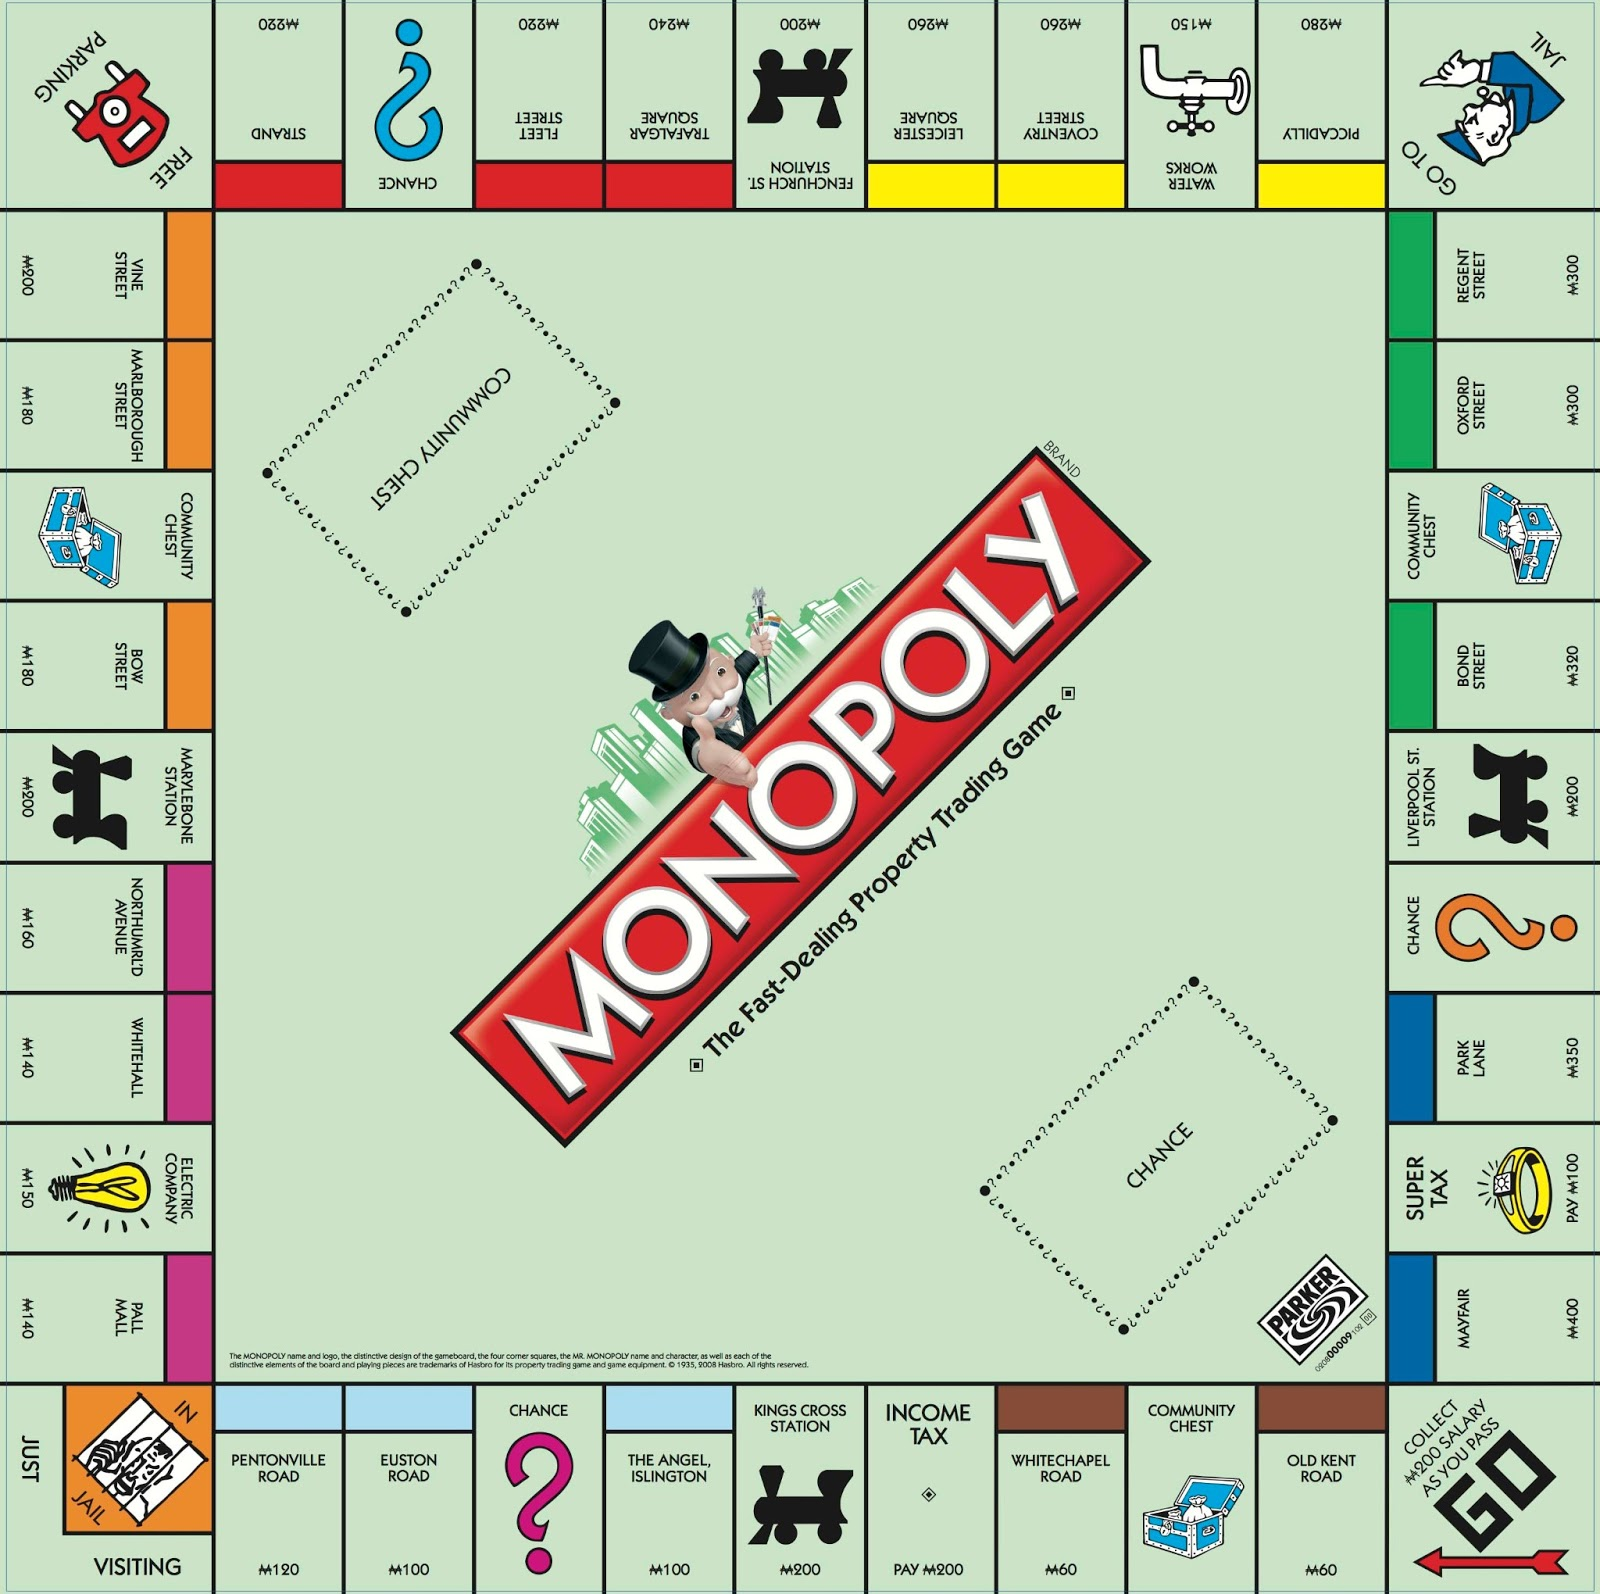
\includegraphics{monopoly_1.jpg}
\caption{monopoly}
\end{figure}

    \hypertarget{goal}{%
\section{Goal}\label{goal}}

    In this document we are going to analyze the probabilities in Monopoly
to answer the question: which are the best houses to buy?

To answer this question we will create a simulated version of Monopoly
and determine the probabilities to land on each square. Then we
calculate the expected value for each square. The squares with the
highest expected values are the best squares to have.

Finally we will create an exact version of our model with a Markov
matrix. We use this to do an error analysis.

    \hypertarget{game-rules}{%
\section{Game rules}\label{game-rules}}

    \hypertarget{squares}{%
\subsection{Squares}\label{squares}}

    Each edge has 9 positions and there are 4 edges. There are 4 corners.
Which gives a total of 40 positions where a player can land. The labels
are numbered starting at GO.

    \hypertarget{labels}{%
\subsubsection{Labels}\label{labels}}

    \begin{Verbatim}[commandchars=\\\{\}]
{\color{incolor}In [{\color{incolor}4}]:} \PY{n}{squares\PYZus{}labels} \PY{o}{=} \PY{p}{[}\PY{l+s+s1}{\PYZsq{}}\PY{l+s+s1}{start}\PY{l+s+s1}{\PYZsq{}}\PY{p}{,} \PY{l+s+s1}{\PYZsq{}}\PY{l+s+s1}{b1}\PY{l+s+s1}{\PYZsq{}}\PY{p}{,} \PY{l+s+s1}{\PYZsq{}}\PY{l+s+s1}{cc1}\PY{l+s+s1}{\PYZsq{}}\PY{p}{,} \PY{l+s+s1}{\PYZsq{}}\PY{l+s+s1}{b2}\PY{l+s+s1}{\PYZsq{}}\PY{p}{,} \PY{l+s+s1}{\PYZsq{}}\PY{l+s+s1}{it}\PY{l+s+s1}{\PYZsq{}}\PY{p}{,} \PY{l+s+s1}{\PYZsq{}}\PY{l+s+s1}{t1}\PY{l+s+s1}{\PYZsq{}}\PY{p}{,} 
                          \PY{l+s+s1}{\PYZsq{}}\PY{l+s+s1}{lb1}\PY{l+s+s1}{\PYZsq{}}\PY{p}{,} \PY{l+s+s1}{\PYZsq{}}\PY{l+s+s1}{c1}\PY{l+s+s1}{\PYZsq{}}\PY{p}{,} \PY{l+s+s1}{\PYZsq{}}\PY{l+s+s1}{lb2}\PY{l+s+s1}{\PYZsq{}}\PY{p}{,} \PY{l+s+s1}{\PYZsq{}}\PY{l+s+s1}{lb3}\PY{l+s+s1}{\PYZsq{}}\PY{p}{,} \PY{l+s+s1}{\PYZsq{}}\PY{l+s+s1}{jail}\PY{l+s+s1}{\PYZsq{}}\PY{p}{,} \PY{l+s+s1}{\PYZsq{}}\PY{l+s+s1}{p1}\PY{l+s+s1}{\PYZsq{}}\PY{p}{,} 
                          \PY{l+s+s1}{\PYZsq{}}\PY{l+s+s1}{ec}\PY{l+s+s1}{\PYZsq{}}\PY{p}{,} \PY{l+s+s1}{\PYZsq{}}\PY{l+s+s1}{p2}\PY{l+s+s1}{\PYZsq{}}\PY{p}{,} \PY{l+s+s1}{\PYZsq{}}\PY{l+s+s1}{p3}\PY{l+s+s1}{\PYZsq{}}\PY{p}{,} \PY{l+s+s1}{\PYZsq{}}\PY{l+s+s1}{ts2}\PY{l+s+s1}{\PYZsq{}}\PY{p}{,} \PY{l+s+s1}{\PYZsq{}}\PY{l+s+s1}{o1}\PY{l+s+s1}{\PYZsq{}}\PY{p}{,} \PY{l+s+s1}{\PYZsq{}}\PY{l+s+s1}{cc2}\PY{l+s+s1}{\PYZsq{}}\PY{p}{,} 
                          \PY{l+s+s1}{\PYZsq{}}\PY{l+s+s1}{o2}\PY{l+s+s1}{\PYZsq{}}\PY{p}{,} \PY{l+s+s1}{\PYZsq{}}\PY{l+s+s1}{o3}\PY{l+s+s1}{\PYZsq{}}\PY{p}{,} \PY{l+s+s1}{\PYZsq{}}\PY{l+s+s1}{p}\PY{l+s+s1}{\PYZsq{}}\PY{p}{,} \PY{l+s+s1}{\PYZsq{}}\PY{l+s+s1}{r1}\PY{l+s+s1}{\PYZsq{}}\PY{p}{,} \PY{l+s+s1}{\PYZsq{}}\PY{l+s+s1}{c2}\PY{l+s+s1}{\PYZsq{}}\PY{p}{,} \PY{l+s+s1}{\PYZsq{}}\PY{l+s+s1}{r2}\PY{l+s+s1}{\PYZsq{}}\PY{p}{,} \PY{l+s+s1}{\PYZsq{}}\PY{l+s+s1}{r3}\PY{l+s+s1}{\PYZsq{}}\PY{p}{,} 
                          \PY{l+s+s1}{\PYZsq{}}\PY{l+s+s1}{ts3}\PY{l+s+s1}{\PYZsq{}}\PY{p}{,} \PY{l+s+s1}{\PYZsq{}}\PY{l+s+s1}{y1}\PY{l+s+s1}{\PYZsq{}}\PY{p}{,} \PY{l+s+s1}{\PYZsq{}}\PY{l+s+s1}{y2}\PY{l+s+s1}{\PYZsq{}}\PY{p}{,} \PY{l+s+s1}{\PYZsq{}}\PY{l+s+s1}{ww}\PY{l+s+s1}{\PYZsq{}}\PY{p}{,} \PY{l+s+s1}{\PYZsq{}}\PY{l+s+s1}{y3}\PY{l+s+s1}{\PYZsq{}}\PY{p}{,} \PY{l+s+s1}{\PYZsq{}}\PY{l+s+s1}{gtj}\PY{l+s+s1}{\PYZsq{}}\PY{p}{,} 
                          \PY{l+s+s1}{\PYZsq{}}\PY{l+s+s1}{g1}\PY{l+s+s1}{\PYZsq{}}\PY{p}{,} \PY{l+s+s1}{\PYZsq{}}\PY{l+s+s1}{g2}\PY{l+s+s1}{\PYZsq{}}\PY{p}{,} \PY{l+s+s1}{\PYZsq{}}\PY{l+s+s1}{cc3}\PY{l+s+s1}{\PYZsq{}}\PY{p}{,} \PY{l+s+s1}{\PYZsq{}}\PY{l+s+s1}{g3}\PY{l+s+s1}{\PYZsq{}}\PY{p}{,} \PY{l+s+s1}{\PYZsq{}}\PY{l+s+s1}{ts4}\PY{l+s+s1}{\PYZsq{}}\PY{p}{,} \PY{l+s+s1}{\PYZsq{}}\PY{l+s+s1}{c3}\PY{l+s+s1}{\PYZsq{}}\PY{p}{,} 
                          \PY{l+s+s1}{\PYZsq{}}\PY{l+s+s1}{db1}\PY{l+s+s1}{\PYZsq{}}\PY{p}{,} \PY{l+s+s1}{\PYZsq{}}\PY{l+s+s1}{st}\PY{l+s+s1}{\PYZsq{}}\PY{p}{,} \PY{l+s+s1}{\PYZsq{}}\PY{l+s+s1}{db2}\PY{l+s+s1}{\PYZsq{}}\PY{p}{]}
        
        \PY{n}{squares\PYZus{}total} \PY{o}{=} \PY{n+nb}{len}\PY{p}{(}\PY{n}{squares\PYZus{}labels}\PY{p}{)}
        \PY{n+nb}{print}\PY{p}{(}\PY{l+s+s1}{\PYZsq{}}\PY{l+s+s1}{There are }\PY{l+s+si}{\PYZob{}\PYZcb{}}\PY{l+s+s1}{ squares.}\PY{l+s+s1}{\PYZsq{}}\PY{o}{.}\PY{n}{format}\PY{p}{(}\PY{n}{squares\PYZus{}total}\PY{p}{)}\PY{p}{)}
\end{Verbatim}


    \begin{Verbatim}[commandchars=\\\{\}]
There are 40 squares.

    \end{Verbatim}

    \hypertarget{descriptions}{%
\subsubsection{Descriptions}\label{descriptions}}

    We also want to know the proper names, so we don't have to look up the
labels.

    \begin{Verbatim}[commandchars=\\\{\}]
{\color{incolor}In [{\color{incolor}5}]:} \PY{n}{squares\PYZus{}description} \PY{o}{=} \PY{p}{[}\PY{l+s+s1}{\PYZsq{}}\PY{l+s+s1}{Start}\PY{l+s+s1}{\PYZsq{}}\PY{p}{,} \PY{l+s+s1}{\PYZsq{}}\PY{l+s+s1}{Brown 1}\PY{l+s+s1}{\PYZsq{}}\PY{p}{,} \PY{l+s+s1}{\PYZsq{}}\PY{l+s+s1}{Community Chest 1}\PY{l+s+s1}{\PYZsq{}}\PY{p}{,} \PY{l+s+s1}{\PYZsq{}}\PY{l+s+s1}{Brown 2}\PY{l+s+s1}{\PYZsq{}}\PY{p}{,} 
                               \PY{l+s+s1}{\PYZsq{}}\PY{l+s+s1}{Income Tax}\PY{l+s+s1}{\PYZsq{}}\PY{p}{,} \PY{l+s+s1}{\PYZsq{}}\PY{l+s+s1}{Train Station 1}\PY{l+s+s1}{\PYZsq{}}\PY{p}{,} \PY{l+s+s1}{\PYZsq{}}\PY{l+s+s1}{Light Blue 1}\PY{l+s+s1}{\PYZsq{}}\PY{p}{,} 
                               \PY{l+s+s1}{\PYZsq{}}\PY{l+s+s1}{Chance 1}\PY{l+s+s1}{\PYZsq{}}\PY{p}{,} \PY{l+s+s1}{\PYZsq{}}\PY{l+s+s1}{Light Blue 2}\PY{l+s+s1}{\PYZsq{}}\PY{p}{,} \PY{l+s+s1}{\PYZsq{}}\PY{l+s+s1}{Light Blue 3}\PY{l+s+s1}{\PYZsq{}}\PY{p}{,} \PY{l+s+s1}{\PYZsq{}}\PY{l+s+s1}{Jail}\PY{l+s+s1}{\PYZsq{}}\PY{p}{,} 
                               \PY{l+s+s1}{\PYZsq{}}\PY{l+s+s1}{Purple 1}\PY{l+s+s1}{\PYZsq{}}\PY{p}{,} \PY{l+s+s1}{\PYZsq{}}\PY{l+s+s1}{Electric Company}\PY{l+s+s1}{\PYZsq{}}\PY{p}{,} \PY{l+s+s1}{\PYZsq{}}\PY{l+s+s1}{Purple 2}\PY{l+s+s1}{\PYZsq{}}\PY{p}{,} 
                               \PY{l+s+s1}{\PYZsq{}}\PY{l+s+s1}{Purple 3}\PY{l+s+s1}{\PYZsq{}}\PY{p}{,} \PY{l+s+s1}{\PYZsq{}}\PY{l+s+s1}{Train Station 2}\PY{l+s+s1}{\PYZsq{}}\PY{p}{,} \PY{l+s+s1}{\PYZsq{}}\PY{l+s+s1}{Orange 1}\PY{l+s+s1}{\PYZsq{}}\PY{p}{,} 
                               \PY{l+s+s1}{\PYZsq{}}\PY{l+s+s1}{Community Chest 2}\PY{l+s+s1}{\PYZsq{}}\PY{p}{,} \PY{l+s+s1}{\PYZsq{}}\PY{l+s+s1}{Orange 2}\PY{l+s+s1}{\PYZsq{}}\PY{p}{,} \PY{l+s+s1}{\PYZsq{}}\PY{l+s+s1}{Orange 3}\PY{l+s+s1}{\PYZsq{}}\PY{p}{,} 
                               \PY{l+s+s1}{\PYZsq{}}\PY{l+s+s1}{Free Parking}\PY{l+s+s1}{\PYZsq{}}\PY{p}{,} \PY{l+s+s1}{\PYZsq{}}\PY{l+s+s1}{Red 1}\PY{l+s+s1}{\PYZsq{}}\PY{p}{,} \PY{l+s+s1}{\PYZsq{}}\PY{l+s+s1}{Chance 2}\PY{l+s+s1}{\PYZsq{}}\PY{p}{,} \PY{l+s+s1}{\PYZsq{}}\PY{l+s+s1}{Red 2}\PY{l+s+s1}{\PYZsq{}}\PY{p}{,} 
                               \PY{l+s+s1}{\PYZsq{}}\PY{l+s+s1}{Red 3}\PY{l+s+s1}{\PYZsq{}}\PY{p}{,} \PY{l+s+s1}{\PYZsq{}}\PY{l+s+s1}{Train Station 3}\PY{l+s+s1}{\PYZsq{}}\PY{p}{,} \PY{l+s+s1}{\PYZsq{}}\PY{l+s+s1}{Yellow 1}\PY{l+s+s1}{\PYZsq{}}\PY{p}{,} \PY{l+s+s1}{\PYZsq{}}\PY{l+s+s1}{Yellow 2}\PY{l+s+s1}{\PYZsq{}}\PY{p}{,} 
                               \PY{l+s+s1}{\PYZsq{}}\PY{l+s+s1}{Water Works}\PY{l+s+s1}{\PYZsq{}}\PY{p}{,} \PY{l+s+s1}{\PYZsq{}}\PY{l+s+s1}{Yellow 3}\PY{l+s+s1}{\PYZsq{}}\PY{p}{,} \PY{l+s+s1}{\PYZsq{}}\PY{l+s+s1}{Go to Jail}\PY{l+s+s1}{\PYZsq{}}\PY{p}{,} \PY{l+s+s1}{\PYZsq{}}\PY{l+s+s1}{Green 1}\PY{l+s+s1}{\PYZsq{}}\PY{p}{,} 
                               \PY{l+s+s1}{\PYZsq{}}\PY{l+s+s1}{Green 2}\PY{l+s+s1}{\PYZsq{}}\PY{p}{,} \PY{l+s+s1}{\PYZsq{}}\PY{l+s+s1}{Community Chest 3}\PY{l+s+s1}{\PYZsq{}}\PY{p}{,} \PY{l+s+s1}{\PYZsq{}}\PY{l+s+s1}{Green 3}\PY{l+s+s1}{\PYZsq{}}\PY{p}{,} 
                               \PY{l+s+s1}{\PYZsq{}}\PY{l+s+s1}{Train Station 4}\PY{l+s+s1}{\PYZsq{}}\PY{p}{,} \PY{l+s+s1}{\PYZsq{}}\PY{l+s+s1}{Chance 3}\PY{l+s+s1}{\PYZsq{}}\PY{p}{,} \PY{l+s+s1}{\PYZsq{}}\PY{l+s+s1}{Dark Blue 1}\PY{l+s+s1}{\PYZsq{}}\PY{p}{,} 
                               \PY{l+s+s1}{\PYZsq{}}\PY{l+s+s1}{Super Tax}\PY{l+s+s1}{\PYZsq{}}\PY{p}{,} \PY{l+s+s1}{\PYZsq{}}\PY{l+s+s1}{Dark Blue 2}\PY{l+s+s1}{\PYZsq{}}\PY{p}{]}
\end{Verbatim}


    \begin{Verbatim}[commandchars=\\\{\}]
{\color{incolor}In [{\color{incolor}6}]:} \PY{n+nb}{print}\PY{p}{(}\PY{l+s+s1}{\PYZsq{}}\PY{l+s+s1}{There are }\PY{l+s+si}{\PYZob{}\PYZcb{}}\PY{l+s+s1}{ descriptions.}\PY{l+s+s1}{\PYZsq{}}\PY{o}{.}\PY{n}{format}\PY{p}{(}\PY{n+nb}{len}\PY{p}{(}\PY{n}{squares\PYZus{}description}\PY{p}{)}\PY{p}{)}\PY{p}{)}
\end{Verbatim}


    \begin{Verbatim}[commandchars=\\\{\}]
There are 40 descriptions.

    \end{Verbatim}

    \hypertarget{purchasable}{%
\subsubsection{Purchasable}\label{purchasable}}

    We want to know if they are purchasable so we can sort on that later.

    \begin{Verbatim}[commandchars=\\\{\}]
{\color{incolor}In [{\color{incolor}7}]:} \PY{n}{squares\PYZus{}purchasable} \PY{o}{=} \PY{p}{[}\PY{k+kc}{False}\PY{p}{,} \PY{k+kc}{True}\PY{p}{,} \PY{k+kc}{False}\PY{p}{,} \PY{k+kc}{True}\PY{p}{,} \PY{k+kc}{False}\PY{p}{,} 
                               \PY{k+kc}{True}\PY{p}{,} \PY{k+kc}{True}\PY{p}{,} \PY{k+kc}{False}\PY{p}{,} \PY{k+kc}{True}\PY{p}{,} \PY{k+kc}{True}\PY{p}{,} 
                               \PY{k+kc}{False}\PY{p}{,} \PY{k+kc}{True}\PY{p}{,} \PY{k+kc}{True}\PY{p}{,} \PY{k+kc}{True}\PY{p}{,} \PY{k+kc}{True}\PY{p}{,} 
                               \PY{k+kc}{True}\PY{p}{,} \PY{k+kc}{True}\PY{p}{,} \PY{k+kc}{False}\PY{p}{,} \PY{k+kc}{True}\PY{p}{,} \PY{k+kc}{True}\PY{p}{,} 
                               \PY{k+kc}{False}\PY{p}{,} \PY{k+kc}{True}\PY{p}{,} \PY{k+kc}{False}\PY{p}{,} \PY{k+kc}{True}\PY{p}{,} \PY{k+kc}{True}\PY{p}{,} 
                               \PY{k+kc}{True}\PY{p}{,} \PY{k+kc}{True}\PY{p}{,} \PY{k+kc}{True}\PY{p}{,} \PY{k+kc}{True}\PY{p}{,} \PY{k+kc}{True}\PY{p}{,} 
                               \PY{k+kc}{False}\PY{p}{,} \PY{k+kc}{True}\PY{p}{,} \PY{k+kc}{True}\PY{p}{,} \PY{k+kc}{False}\PY{p}{,} \PY{k+kc}{True}\PY{p}{,} 
                               \PY{k+kc}{True}\PY{p}{,} \PY{k+kc}{False}\PY{p}{,} \PY{k+kc}{True}\PY{p}{,} \PY{k+kc}{False}\PY{p}{,} \PY{k+kc}{True}\PY{p}{]}
\end{Verbatim}


    \hypertarget{rent}{%
\subsubsection{Rent}\label{rent}}

    We want to use the rent paid at each square to calculate the expected
value. The utility company charge \(4\) times roll if one is owned, and
\(10\) times roll if both owned. For one railway we charge \(\$25\), two
\(\$50\), three \(\$100\), and all four \(\$200\).

    To find the rent for a utility company, we find the expected value for
throwing a dices times \(4\).

\[ 4\cdot E(\bar{k}) = 4 \cdot \dfrac{1}{6} \cdot (1+2+3+4+5+6) \]

    \begin{Verbatim}[commandchars=\\\{\}]
{\color{incolor}In [{\color{incolor}8}]:} \PY{n}{E\PYZus{}u} \PY{o}{=} \PY{l+m+mi}{4} \PY{o}{*} \PY{p}{(}\PY{l+m+mi}{1}\PY{o}{+}\PY{l+m+mi}{2}\PY{o}{+}\PY{l+m+mi}{3}\PY{o}{+}\PY{l+m+mi}{4}\PY{o}{+}\PY{l+m+mi}{5}\PY{o}{+}\PY{l+m+mi}{6}\PY{p}{)} \PY{o}{/} \PY{l+m+mi}{6}
\end{Verbatim}


    We pick the value for one railway which is \(25\).

    \begin{Verbatim}[commandchars=\\\{\}]
{\color{incolor}In [{\color{incolor}9}]:} \PY{n}{E\PYZus{}r} \PY{o}{=} \PY{l+m+mi}{25}
\end{Verbatim}


    \begin{Verbatim}[commandchars=\\\{\}]
{\color{incolor}In [{\color{incolor}10}]:} \PY{n}{squares\PYZus{}rent} \PY{o}{=} \PY{p}{[}\PY{l+m+mi}{0}\PY{p}{,} \PY{l+m+mi}{2}\PY{p}{,} \PY{l+m+mi}{0}\PY{p}{,} \PY{l+m+mi}{4}\PY{p}{,} \PY{l+m+mi}{0}\PY{p}{,} \PY{n}{E\PYZus{}r}\PY{p}{,} \PY{l+m+mi}{6}\PY{p}{,} \PY{l+m+mi}{0}\PY{p}{,} \PY{l+m+mi}{6}\PY{p}{,} \PY{l+m+mi}{8}\PY{p}{,} \PY{l+m+mi}{0}\PY{p}{,} \PY{l+m+mi}{10}\PY{p}{,} \PY{n}{E\PYZus{}u}\PY{p}{,} 
                         \PY{l+m+mi}{10}\PY{p}{,} \PY{l+m+mi}{12}\PY{p}{,} \PY{n}{E\PYZus{}r}\PY{p}{,} \PY{l+m+mi}{14}\PY{p}{,} \PY{l+m+mi}{0}\PY{p}{,} \PY{l+m+mi}{14}\PY{p}{,} \PY{l+m+mi}{16}\PY{p}{,} \PY{l+m+mi}{0}\PY{p}{,} \PY{l+m+mi}{18}\PY{p}{,} \PY{l+m+mi}{0}\PY{p}{,} \PY{l+m+mi}{18}\PY{p}{,} 
                         \PY{l+m+mi}{20}\PY{p}{,} \PY{n}{E\PYZus{}r}\PY{p}{,} \PY{l+m+mi}{22}\PY{p}{,} \PY{l+m+mi}{22}\PY{p}{,} \PY{n}{E\PYZus{}u}\PY{p}{,} \PY{l+m+mi}{24}\PY{p}{,} \PY{l+m+mi}{0}\PY{p}{,} \PY{l+m+mi}{26}\PY{p}{,} \PY{l+m+mi}{26}\PY{p}{,} \PY{l+m+mi}{0}\PY{p}{,} \PY{l+m+mi}{28}\PY{p}{,} 
                         \PY{n}{E\PYZus{}r}\PY{p}{,} \PY{l+m+mi}{0}\PY{p}{,} \PY{l+m+mi}{35}\PY{p}{,} \PY{l+m+mi}{0}\PY{p}{,} \PY{l+m+mi}{50}\PY{p}{]}
\end{Verbatim}


    \hypertarget{grouping}{%
\subsubsection{Grouping}\label{grouping}}

    We want to know in what group they are so we can aggregate our data
later.

    \begin{Verbatim}[commandchars=\\\{\}]
{\color{incolor}In [{\color{incolor}11}]:} \PY{n}{squares\PYZus{}aggregate} \PY{o}{=} \PY{p}{[}\PY{l+s+s1}{\PYZsq{}}\PY{l+s+s1}{Start}\PY{l+s+s1}{\PYZsq{}}\PY{p}{,} \PY{l+s+s1}{\PYZsq{}}\PY{l+s+s1}{Brown}\PY{l+s+s1}{\PYZsq{}}\PY{p}{,} \PY{l+s+s1}{\PYZsq{}}\PY{l+s+s1}{Community Chest}\PY{l+s+s1}{\PYZsq{}}\PY{p}{,} \PY{l+s+s1}{\PYZsq{}}\PY{l+s+s1}{Brown}\PY{l+s+s1}{\PYZsq{}}\PY{p}{,} 
                              \PY{l+s+s1}{\PYZsq{}}\PY{l+s+s1}{Income Tax}\PY{l+s+s1}{\PYZsq{}}\PY{p}{,} \PY{l+s+s1}{\PYZsq{}}\PY{l+s+s1}{Train Station}\PY{l+s+s1}{\PYZsq{}}\PY{p}{,} \PY{l+s+s1}{\PYZsq{}}\PY{l+s+s1}{Light Blue}\PY{l+s+s1}{\PYZsq{}}\PY{p}{,} 
                              \PY{l+s+s1}{\PYZsq{}}\PY{l+s+s1}{Chance}\PY{l+s+s1}{\PYZsq{}}\PY{p}{,} \PY{l+s+s1}{\PYZsq{}}\PY{l+s+s1}{Light Blue}\PY{l+s+s1}{\PYZsq{}}\PY{p}{,} \PY{l+s+s1}{\PYZsq{}}\PY{l+s+s1}{Light Blue}\PY{l+s+s1}{\PYZsq{}}\PY{p}{,} \PY{l+s+s1}{\PYZsq{}}\PY{l+s+s1}{Jail}\PY{l+s+s1}{\PYZsq{}}\PY{p}{,} 
                              \PY{l+s+s1}{\PYZsq{}}\PY{l+s+s1}{Purple}\PY{l+s+s1}{\PYZsq{}}\PY{p}{,} \PY{l+s+s1}{\PYZsq{}}\PY{l+s+s1}{Utilities}\PY{l+s+s1}{\PYZsq{}}\PY{p}{,} \PY{l+s+s1}{\PYZsq{}}\PY{l+s+s1}{Purple}\PY{l+s+s1}{\PYZsq{}}\PY{p}{,} \PY{l+s+s1}{\PYZsq{}}\PY{l+s+s1}{Purple}\PY{l+s+s1}{\PYZsq{}}\PY{p}{,} 
                              \PY{l+s+s1}{\PYZsq{}}\PY{l+s+s1}{Train Station}\PY{l+s+s1}{\PYZsq{}}\PY{p}{,} \PY{l+s+s1}{\PYZsq{}}\PY{l+s+s1}{Orange}\PY{l+s+s1}{\PYZsq{}}\PY{p}{,} \PY{l+s+s1}{\PYZsq{}}\PY{l+s+s1}{Community Chest}\PY{l+s+s1}{\PYZsq{}}\PY{p}{,} 
                              \PY{l+s+s1}{\PYZsq{}}\PY{l+s+s1}{Orange}\PY{l+s+s1}{\PYZsq{}}\PY{p}{,} \PY{l+s+s1}{\PYZsq{}}\PY{l+s+s1}{Orange}\PY{l+s+s1}{\PYZsq{}}\PY{p}{,} \PY{l+s+s1}{\PYZsq{}}\PY{l+s+s1}{Free Parking}\PY{l+s+s1}{\PYZsq{}}\PY{p}{,} \PY{l+s+s1}{\PYZsq{}}\PY{l+s+s1}{Red}\PY{l+s+s1}{\PYZsq{}}\PY{p}{,} 
                              \PY{l+s+s1}{\PYZsq{}}\PY{l+s+s1}{Chance}\PY{l+s+s1}{\PYZsq{}}\PY{p}{,} \PY{l+s+s1}{\PYZsq{}}\PY{l+s+s1}{Red}\PY{l+s+s1}{\PYZsq{}}\PY{p}{,} \PY{l+s+s1}{\PYZsq{}}\PY{l+s+s1}{Red}\PY{l+s+s1}{\PYZsq{}}\PY{p}{,} \PY{l+s+s1}{\PYZsq{}}\PY{l+s+s1}{Train Station}\PY{l+s+s1}{\PYZsq{}}\PY{p}{,} \PY{l+s+s1}{\PYZsq{}}\PY{l+s+s1}{Yellow}\PY{l+s+s1}{\PYZsq{}}\PY{p}{,} 
                              \PY{l+s+s1}{\PYZsq{}}\PY{l+s+s1}{Yellow}\PY{l+s+s1}{\PYZsq{}}\PY{p}{,} \PY{l+s+s1}{\PYZsq{}}\PY{l+s+s1}{Utilities}\PY{l+s+s1}{\PYZsq{}}\PY{p}{,} \PY{l+s+s1}{\PYZsq{}}\PY{l+s+s1}{Yellow}\PY{l+s+s1}{\PYZsq{}}\PY{p}{,} \PY{l+s+s1}{\PYZsq{}}\PY{l+s+s1}{Go to Jail}\PY{l+s+s1}{\PYZsq{}}\PY{p}{,} 
                              \PY{l+s+s1}{\PYZsq{}}\PY{l+s+s1}{Green}\PY{l+s+s1}{\PYZsq{}}\PY{p}{,} \PY{l+s+s1}{\PYZsq{}}\PY{l+s+s1}{Green}\PY{l+s+s1}{\PYZsq{}}\PY{p}{,} \PY{l+s+s1}{\PYZsq{}}\PY{l+s+s1}{Community Chest}\PY{l+s+s1}{\PYZsq{}}\PY{p}{,} \PY{l+s+s1}{\PYZsq{}}\PY{l+s+s1}{Green}\PY{l+s+s1}{\PYZsq{}}\PY{p}{,} 
                              \PY{l+s+s1}{\PYZsq{}}\PY{l+s+s1}{Train Station}\PY{l+s+s1}{\PYZsq{}}\PY{p}{,} \PY{l+s+s1}{\PYZsq{}}\PY{l+s+s1}{Chance}\PY{l+s+s1}{\PYZsq{}}\PY{p}{,} \PY{l+s+s1}{\PYZsq{}}\PY{l+s+s1}{Dark Blue}\PY{l+s+s1}{\PYZsq{}}\PY{p}{,} 
                              \PY{l+s+s1}{\PYZsq{}}\PY{l+s+s1}{Super Tax}\PY{l+s+s1}{\PYZsq{}}\PY{p}{,} \PY{l+s+s1}{\PYZsq{}}\PY{l+s+s1}{Dark Blue}\PY{l+s+s1}{\PYZsq{}}\PY{p}{]}
\end{Verbatim}


    \hypertarget{cards}{%
\subsection{Cards}\label{cards}}

    There are two decks of cards.

\begin{itemize}
\tightlist
\item
  Community Cards
\item
  Chance Cards
\end{itemize}

Each deck contains 16 cards.

    \hypertarget{community-cards}{%
\subsubsection{Community Cards}\label{community-cards}}

    Monopoly has \(16\) community cards.

    \begin{figure}
\centering
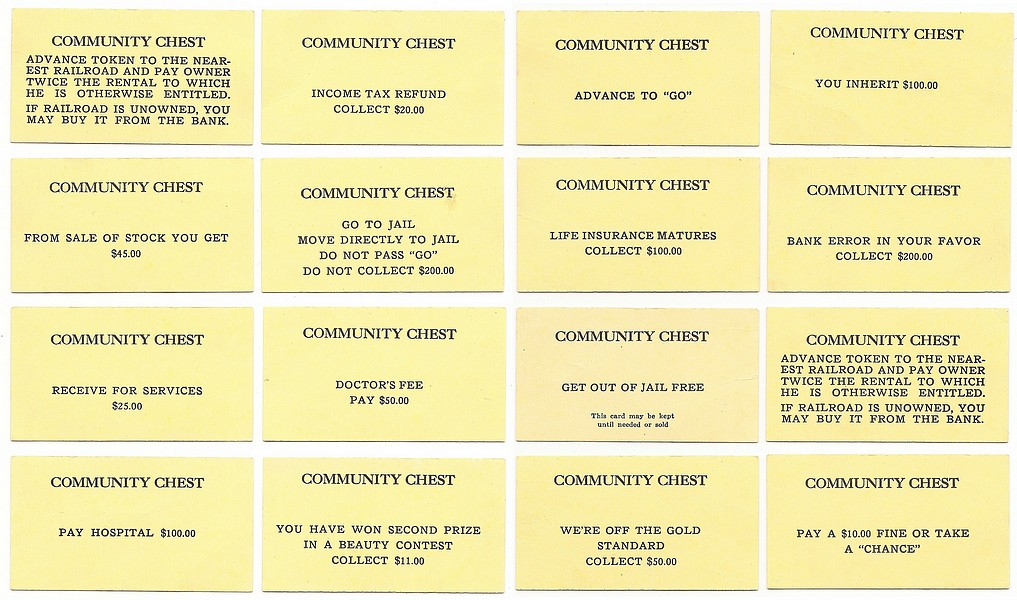
\includegraphics{monopoly_2.jpg}
\caption{cc}
\end{figure}

    Because we are only determining the probabilities, we are only
interested in the following cards:

\begin{itemize}
\tightlist
\item
  advance to go
\item
  go to jail
\item
  get out of jail, free
\item
  go back 2 spaces
\end{itemize}

    \hypertarget{community-deck-implementation}{%
\subsubsection{Community deck
implementation}\label{community-deck-implementation}}

    We implement the community deck in a class. The class keeps track of a
list with \(16\) cards. An index points to the next card. When we are
out of cards, we reset the index and reshuffle the cards.

    \begin{Verbatim}[commandchars=\\\{\}]
{\color{incolor}In [{\color{incolor}12}]:} \PY{k+kn}{from} \PY{n+nn}{random} \PY{k}{import} \PY{n}{shuffle}
         
         \PY{k}{class} \PY{n+nc}{CommunityDeck}\PY{p}{(}\PY{p}{)}\PY{p}{:}
             \PY{k}{def} \PY{n+nf}{\PYZus{}\PYZus{}init\PYZus{}\PYZus{}}\PY{p}{(}\PY{n+nb+bp}{self}\PY{p}{)}\PY{p}{:}
                 \PY{n+nb+bp}{self}\PY{o}{.}\PY{n}{deck} \PY{o}{=} \PY{p}{[}\PY{l+m+mi}{0}\PY{p}{]} \PY{o}{*} \PY{l+m+mi}{16}
                 \PY{n+nb+bp}{self}\PY{o}{.}\PY{n}{deck}\PY{p}{[}\PY{l+m+mi}{0}\PY{p}{]} \PY{o}{=} \PY{l+s+s1}{\PYZsq{}}\PY{l+s+s1}{gtg}\PY{l+s+s1}{\PYZsq{}} \PY{c+c1}{\PYZsh{} go to go}
                 \PY{n+nb+bp}{self}\PY{o}{.}\PY{n}{deck}\PY{p}{[}\PY{l+m+mi}{1}\PY{p}{]} \PY{o}{=} \PY{l+s+s1}{\PYZsq{}}\PY{l+s+s1}{gtj}\PY{l+s+s1}{\PYZsq{}} \PY{c+c1}{\PYZsh{} go to jail}
                 \PY{n+nb+bp}{self}\PY{o}{.}\PY{n}{deck}\PY{p}{[}\PY{l+m+mi}{2}\PY{p}{]} \PY{o}{=} \PY{l+s+s1}{\PYZsq{}}\PY{l+s+s1}{goj}\PY{l+s+s1}{\PYZsq{}} \PY{c+c1}{\PYZsh{} get out of jail }
                 \PY{n+nb+bp}{self}\PY{o}{.}\PY{n}{deck}\PY{p}{[}\PY{l+m+mi}{3}\PY{p}{]} \PY{o}{=} \PY{l+s+s1}{\PYZsq{}}\PY{l+s+s1}{gb2}\PY{l+s+s1}{\PYZsq{}} \PY{c+c1}{\PYZsh{} go back 2 steps}
                 \PY{n+nb+bp}{self}\PY{o}{.}\PY{n}{index} \PY{o}{=} \PY{l+m+mi}{16}
             
             \PY{k}{def} \PY{n+nf}{draw\PYZus{}card}\PY{p}{(}\PY{n+nb+bp}{self}\PY{p}{)}\PY{p}{:}
                 \PY{k}{if} \PY{n+nb+bp}{self}\PY{o}{.}\PY{n}{index} \PY{o}{\PYZgt{}}\PY{o}{=} \PY{n+nb}{len}\PY{p}{(}\PY{n+nb+bp}{self}\PY{o}{.}\PY{n}{deck}\PY{p}{)}\PY{p}{:}
                     \PY{n+nb+bp}{self}\PY{o}{.}\PY{n}{index} \PY{o}{=} \PY{l+m+mi}{0}
                     \PY{n}{shuffle}\PY{p}{(}\PY{n+nb+bp}{self}\PY{o}{.}\PY{n}{deck}\PY{p}{)}
                 \PY{n}{card} \PY{o}{=} \PY{n+nb+bp}{self}\PY{o}{.}\PY{n}{deck}\PY{p}{[}\PY{n+nb+bp}{self}\PY{o}{.}\PY{n}{index}\PY{p}{]}
                 \PY{n+nb+bp}{self}\PY{o}{.}\PY{n}{index} \PY{o}{+}\PY{o}{=} \PY{l+m+mi}{1}
                 \PY{k}{return} \PY{n}{card}
\end{Verbatim}


    Now we test it:

    \begin{Verbatim}[commandchars=\\\{\}]
{\color{incolor}In [{\color{incolor}13}]:} \PY{n}{deck} \PY{o}{=} \PY{n}{CommunityDeck}\PY{p}{(}\PY{p}{)}
         \PY{n}{deck}\PY{o}{.}\PY{n}{deck}
\end{Verbatim}


\begin{Verbatim}[commandchars=\\\{\}]
{\color{outcolor}Out[{\color{outcolor}13}]:} ['gtg', 'gtj', 'goj', 'gb2', 0, 0, 0, 0, 0, 0, 0, 0, 0, 0, 0, 0]
\end{Verbatim}
            
    \begin{Verbatim}[commandchars=\\\{\}]
{\color{incolor}In [{\color{incolor}14}]:} \PY{n}{deck}\PY{o}{.}\PY{n}{draw\PYZus{}card}\PY{p}{(}\PY{p}{)}
\end{Verbatim}


\begin{Verbatim}[commandchars=\\\{\}]
{\color{outcolor}Out[{\color{outcolor}14}]:} 0
\end{Verbatim}
            
    \begin{Verbatim}[commandchars=\\\{\}]
{\color{incolor}In [{\color{incolor}15}]:} \PY{n}{deck}\PY{o}{.}\PY{n}{deck}
\end{Verbatim}


\begin{Verbatim}[commandchars=\\\{\}]
{\color{outcolor}Out[{\color{outcolor}15}]:} [0, 0, 0, 'gb2', 0, 'goj', 0, 'gtg', 0, 0, 0, 0, 'gtj', 0, 0, 0]
\end{Verbatim}
            
    \begin{Verbatim}[commandchars=\\\{\}]
{\color{incolor}In [{\color{incolor}16}]:} \PY{n}{deck}\PY{o}{.}\PY{n}{index}
\end{Verbatim}


\begin{Verbatim}[commandchars=\\\{\}]
{\color{outcolor}Out[{\color{outcolor}16}]:} 1
\end{Verbatim}
            
    \hypertarget{chance-cards}{%
\subsubsection{Chance Cards}\label{chance-cards}}

    Monopoly has \(16\) chance cards.

    \begin{figure}
\centering
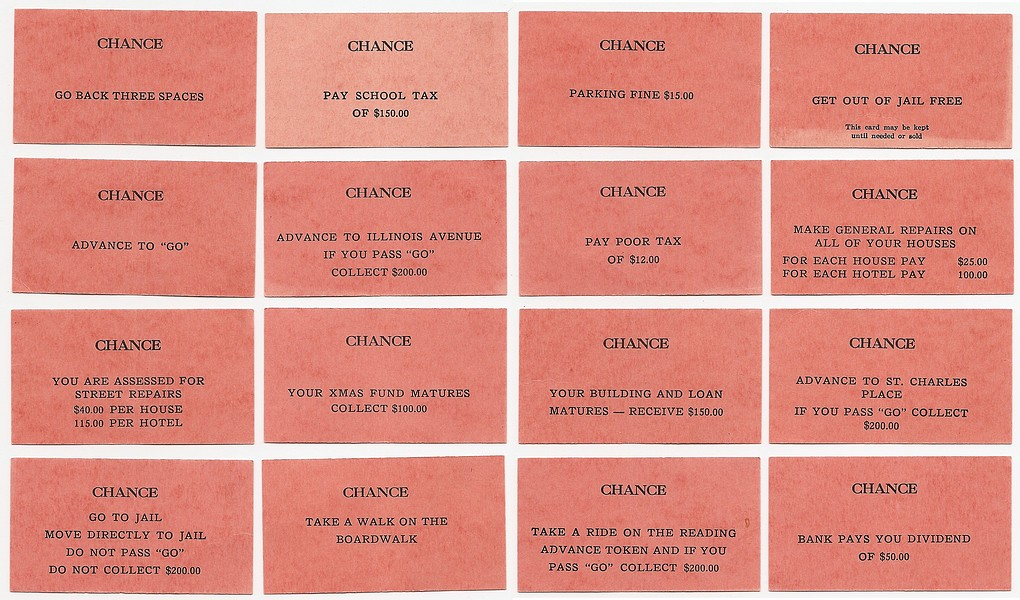
\includegraphics{monopoly_3.jpg}
\caption{chance}
\end{figure}

    Because we are only determining the probabilities, we are only
interested in the following cards:

\begin{itemize}
\tightlist
\item
  go back three spaces
\item
  get out of jail free
\item
  advance to go
\item
  advance to illinois avenue (R3)
\item
  go to jail
\end{itemize}

    \hypertarget{chance-deck-implementation}{%
\subsubsection{Chance deck
implementation}\label{chance-deck-implementation}}

    We implement the chance deck in a class. The class keeps track of a list
with \(16\) cards. An index points to the next card. When we are out of
cards, we reset the index and reshuffle the cards.

    \begin{Verbatim}[commandchars=\\\{\}]
{\color{incolor}In [{\color{incolor}17}]:} \PY{k+kn}{from} \PY{n+nn}{random} \PY{k}{import} \PY{n}{shuffle}
         
         \PY{k}{class} \PY{n+nc}{ChanceDeck}\PY{p}{(}\PY{p}{)}\PY{p}{:}
             \PY{k}{def} \PY{n+nf}{\PYZus{}\PYZus{}init\PYZus{}\PYZus{}}\PY{p}{(}\PY{n+nb+bp}{self}\PY{p}{)}\PY{p}{:}
                 \PY{n+nb+bp}{self}\PY{o}{.}\PY{n}{deck} \PY{o}{=} \PY{p}{[}\PY{l+m+mi}{0}\PY{p}{]} \PY{o}{*} \PY{l+m+mi}{16}
                 \PY{n+nb+bp}{self}\PY{o}{.}\PY{n}{deck}\PY{p}{[}\PY{l+m+mi}{0}\PY{p}{]} \PY{o}{=} \PY{l+s+s1}{\PYZsq{}}\PY{l+s+s1}{gtg}\PY{l+s+s1}{\PYZsq{}} \PY{c+c1}{\PYZsh{} go to go}
                 \PY{n+nb+bp}{self}\PY{o}{.}\PY{n}{deck}\PY{p}{[}\PY{l+m+mi}{1}\PY{p}{]} \PY{o}{=} \PY{l+s+s1}{\PYZsq{}}\PY{l+s+s1}{gtj}\PY{l+s+s1}{\PYZsq{}} \PY{c+c1}{\PYZsh{} go to jail}
                 \PY{n+nb+bp}{self}\PY{o}{.}\PY{n}{deck}\PY{p}{[}\PY{l+m+mi}{2}\PY{p}{]} \PY{o}{=} \PY{l+s+s1}{\PYZsq{}}\PY{l+s+s1}{goj}\PY{l+s+s1}{\PYZsq{}} \PY{c+c1}{\PYZsh{} get out of jail}
                 \PY{c+c1}{\PYZsh{}self.deck[3] = \PYZsq{}gb3\PYZsq{} \PYZsh{} go back 3}
                 \PY{n+nb+bp}{self}\PY{o}{.}\PY{n}{deck}\PY{p}{[}\PY{l+m+mi}{4}\PY{p}{]} \PY{o}{=} \PY{l+s+s1}{\PYZsq{}}\PY{l+s+s1}{r3}\PY{l+s+s1}{\PYZsq{}}  \PY{c+c1}{\PYZsh{} go to red 3 (r3)}
                 \PY{n+nb+bp}{self}\PY{o}{.}\PY{n}{index} \PY{o}{=} \PY{l+m+mi}{16}
             
             \PY{k}{def} \PY{n+nf}{draw\PYZus{}card}\PY{p}{(}\PY{n+nb+bp}{self}\PY{p}{)}\PY{p}{:}
                 \PY{k}{if} \PY{n+nb+bp}{self}\PY{o}{.}\PY{n}{index} \PY{o}{\PYZgt{}}\PY{o}{=} \PY{n+nb}{len}\PY{p}{(}\PY{n+nb+bp}{self}\PY{o}{.}\PY{n}{deck}\PY{p}{)}\PY{p}{:}
                     \PY{n+nb+bp}{self}\PY{o}{.}\PY{n}{index} \PY{o}{=} \PY{l+m+mi}{0}
                     \PY{n}{shuffle}\PY{p}{(}\PY{n+nb+bp}{self}\PY{o}{.}\PY{n}{deck}\PY{p}{)}
                 \PY{n}{card} \PY{o}{=} \PY{n+nb+bp}{self}\PY{o}{.}\PY{n}{deck}\PY{p}{[}\PY{n+nb+bp}{self}\PY{o}{.}\PY{n}{index}\PY{p}{]}
                 \PY{n+nb+bp}{self}\PY{o}{.}\PY{n}{index} \PY{o}{+}\PY{o}{=} \PY{l+m+mi}{1}
                 \PY{k}{return} \PY{n}{card}
\end{Verbatim}


    Now we test it:

    \begin{Verbatim}[commandchars=\\\{\}]
{\color{incolor}In [{\color{incolor}18}]:} \PY{n}{deck} \PY{o}{=} \PY{n}{ChanceDeck}\PY{p}{(}\PY{p}{)}
         \PY{n}{deck}\PY{o}{.}\PY{n}{deck}
\end{Verbatim}


\begin{Verbatim}[commandchars=\\\{\}]
{\color{outcolor}Out[{\color{outcolor}18}]:} ['gtg', 'gtj', 'goj', 0, 'r3', 0, 0, 0, 0, 0, 0, 0, 0, 0, 0, 0]
\end{Verbatim}
            
    \begin{Verbatim}[commandchars=\\\{\}]
{\color{incolor}In [{\color{incolor}19}]:} \PY{n}{deck}\PY{o}{.}\PY{n}{draw\PYZus{}card}\PY{p}{(}\PY{p}{)}
\end{Verbatim}


\begin{Verbatim}[commandchars=\\\{\}]
{\color{outcolor}Out[{\color{outcolor}19}]:} 0
\end{Verbatim}
            
    \begin{Verbatim}[commandchars=\\\{\}]
{\color{incolor}In [{\color{incolor}20}]:} \PY{n}{deck}\PY{o}{.}\PY{n}{deck}
\end{Verbatim}


\begin{Verbatim}[commandchars=\\\{\}]
{\color{outcolor}Out[{\color{outcolor}20}]:} [0, 0, 'gtj', 'gtg', 'goj', 0, 0, 0, 0, 0, 0, 0, 0, 0, 0, 'r3']
\end{Verbatim}
            
    \begin{Verbatim}[commandchars=\\\{\}]
{\color{incolor}In [{\color{incolor}21}]:} \PY{n}{deck}\PY{o}{.}\PY{n}{index}
\end{Verbatim}


\begin{Verbatim}[commandchars=\\\{\}]
{\color{outcolor}Out[{\color{outcolor}21}]:} 1
\end{Verbatim}
            
    \hypertarget{dice}{%
\subsection{Dice}\label{dice}}

    We will be implementing the dice as a class. This allows us to
encapsulate how the result are determined. It makes it easier to
implements other scenarios such as throwing with multiple dices.

    \begin{Verbatim}[commandchars=\\\{\}]
{\color{incolor}In [{\color{incolor}22}]:} \PY{k+kn}{from} \PY{n+nn}{random} \PY{k}{import} \PY{n}{randint}
         
         \PY{k}{class} \PY{n+nc}{Dice}\PY{p}{(}\PY{p}{)}\PY{p}{:}
             \PY{k}{def} \PY{n+nf}{\PYZus{}\PYZus{}init\PYZus{}\PYZus{}}\PY{p}{(}\PY{n+nb+bp}{self}\PY{p}{,} \PY{n}{dices} \PY{o}{=} \PY{l+m+mi}{1}\PY{p}{,} \PY{n}{sides} \PY{o}{=} \PY{l+m+mi}{6}\PY{p}{)}\PY{p}{:}
                 \PY{n+nb+bp}{self}\PY{o}{.}\PY{n}{dices} \PY{o}{=} \PY{n}{dices}
                 \PY{n+nb+bp}{self}\PY{o}{.}\PY{n}{sides} \PY{o}{=} \PY{n}{sides}
             
             \PY{k}{def} \PY{n+nf}{throw}\PY{p}{(}\PY{n+nb+bp}{self}\PY{p}{)}\PY{p}{:}
                 \PY{k}{return} \PY{n+nb}{sum}\PY{p}{(}\PY{p}{[}\PY{n}{randint}\PY{p}{(}\PY{l+m+mi}{1}\PY{p}{,} \PY{n+nb+bp}{self}\PY{o}{.}\PY{n}{sides}\PY{p}{)} \PY{k}{for} \PY{n}{\PYZus{}} \PY{o+ow}{in} \PY{n+nb}{range}\PY{p}{(}\PY{n+nb+bp}{self}\PY{o}{.}\PY{n}{dices}\PY{p}{)}\PY{p}{]}\PY{p}{)}
\end{Verbatim}


    Rolling one time:

    \begin{Verbatim}[commandchars=\\\{\}]
{\color{incolor}In [{\color{incolor}23}]:} \PY{n}{dice} \PY{o}{=} \PY{n}{Dice}\PY{p}{(}\PY{p}{)}
         \PY{n}{dice}\PY{o}{.}\PY{n}{throw}\PY{p}{(}\PY{p}{)}
\end{Verbatim}


\begin{Verbatim}[commandchars=\\\{\}]
{\color{outcolor}Out[{\color{outcolor}23}]:} 5
\end{Verbatim}
            
    \hypertarget{simple-one-dice-with-six-sides}{%
\subsubsection{Simple: one dice with six
sides}\label{simple-one-dice-with-six-sides}}

    A simple setup would be one dice with six sides. This will give
uniformly distributed probabilities.

    \begin{Verbatim}[commandchars=\\\{\}]
{\color{incolor}In [{\color{incolor}24}]:} \PY{n}{dice} \PY{o}{=} \PY{n}{Dice}\PY{p}{(}\PY{p}{)}
         \PY{n}{sides} \PY{o}{=} \PY{p}{[}\PY{l+m+mi}{0}\PY{p}{]} \PY{o}{*} \PY{n}{dice}\PY{o}{.}\PY{n}{dices} \PY{o}{*} \PY{n}{dice}\PY{o}{.}\PY{n}{sides}
         \PY{n}{N} \PY{o}{=} \PY{l+m+mi}{10000}
         \PY{k}{for} \PY{n}{i} \PY{o+ow}{in} \PY{n+nb}{range}\PY{p}{(}\PY{n}{N}\PY{p}{)}\PY{p}{:} \PY{n}{sides}\PY{p}{[}\PY{n}{dice}\PY{o}{.}\PY{n}{throw}\PY{p}{(}\PY{p}{)}\PY{o}{\PYZhy{}}\PY{l+m+mi}{1}\PY{p}{]} \PY{o}{+}\PY{o}{=} \PY{l+m+mi}{1}
         \PY{n}{sides} \PY{o}{=} \PY{n}{np}\PY{o}{.}\PY{n}{array}\PY{p}{(}\PY{n}{sides}\PY{p}{)} \PY{o}{/} \PY{n}{N}
         \PY{n}{bar}\PY{p}{(}\PY{n+nb}{range}\PY{p}{(}\PY{l+m+mi}{1}\PY{p}{,}\PY{n+nb}{len}\PY{p}{(}\PY{n}{sides}\PY{p}{)}\PY{o}{+}\PY{l+m+mi}{1}\PY{p}{)}\PY{p}{,} \PY{n}{sides}\PY{p}{)}\PY{p}{;}
         \PY{n}{ylabel}\PY{p}{(}\PY{l+s+s1}{\PYZsq{}}\PY{l+s+s1}{P(x)}\PY{l+s+s1}{\PYZsq{}}\PY{p}{)}
         \PY{n}{xlabel}\PY{p}{(}\PY{l+s+s1}{\PYZsq{}}\PY{l+s+s1}{x}\PY{l+s+s1}{\PYZsq{}}\PY{p}{)}
         \PY{n}{title}\PY{p}{(}\PY{l+s+s1}{\PYZsq{}}\PY{l+s+s1}{Probability distribution for one dice; N=10,000}\PY{l+s+s1}{\PYZsq{}}\PY{p}{)}\PY{p}{;}
\end{Verbatim}


    \begin{center}
    \adjustimage{max size={0.9\linewidth}{0.9\paperheight}}{output_61_0.png}
    \end{center}
    { \hspace*{\fill} \\}
    
    \hypertarget{advanced-two-dice-with-six-sides}{%
\subsubsection{Advanced: two dice with six
sides}\label{advanced-two-dice-with-six-sides}}

    Monopoly is played with two dices. This will give the following
probability distribution:

    \begin{Verbatim}[commandchars=\\\{\}]
{\color{incolor}In [{\color{incolor}25}]:} \PY{n}{dice} \PY{o}{=} \PY{n}{Dice}\PY{p}{(}\PY{l+m+mi}{2}\PY{p}{)}
         \PY{n}{sides} \PY{o}{=} \PY{p}{[}\PY{l+m+mi}{0}\PY{p}{]} \PY{o}{*} \PY{n}{dice}\PY{o}{.}\PY{n}{dices} \PY{o}{*} \PY{n}{dice}\PY{o}{.}\PY{n}{sides}
         \PY{n}{N} \PY{o}{=} \PY{l+m+mi}{10000}
         \PY{k}{for} \PY{n}{i} \PY{o+ow}{in} \PY{n+nb}{range}\PY{p}{(}\PY{n}{N}\PY{p}{)}\PY{p}{:} \PY{n}{sides}\PY{p}{[}\PY{n}{dice}\PY{o}{.}\PY{n}{throw}\PY{p}{(}\PY{p}{)}\PY{o}{\PYZhy{}}\PY{l+m+mi}{1}\PY{p}{]} \PY{o}{+}\PY{o}{=} \PY{l+m+mi}{1}
         \PY{n}{sides} \PY{o}{=} \PY{n}{np}\PY{o}{.}\PY{n}{array}\PY{p}{(}\PY{n}{sides}\PY{p}{)} \PY{o}{/} \PY{n}{N}
         \PY{n}{bar}\PY{p}{(}\PY{n+nb}{range}\PY{p}{(}\PY{l+m+mi}{1}\PY{p}{,}\PY{n+nb}{len}\PY{p}{(}\PY{n}{sides}\PY{p}{)}\PY{o}{+}\PY{l+m+mi}{1}\PY{p}{)}\PY{p}{,} \PY{n}{sides}\PY{p}{)}\PY{p}{;}
         \PY{n}{ylabel}\PY{p}{(}\PY{l+s+s1}{\PYZsq{}}\PY{l+s+s1}{P(x)}\PY{l+s+s1}{\PYZsq{}}\PY{p}{)}
         \PY{n}{xlabel}\PY{p}{(}\PY{l+s+s1}{\PYZsq{}}\PY{l+s+s1}{x}\PY{l+s+s1}{\PYZsq{}}\PY{p}{)}
         \PY{n}{title}\PY{p}{(}\PY{l+s+s1}{\PYZsq{}}\PY{l+s+s1}{Probability distribution for two dices; N=10,000}\PY{l+s+s1}{\PYZsq{}}\PY{p}{)}\PY{p}{;}
\end{Verbatim}


    \begin{center}
    \adjustimage{max size={0.9\linewidth}{0.9\paperheight}}{output_64_0.png}
    \end{center}
    { \hspace*{\fill} \\}
    
    \hypertarget{monopoly-simulation}{%
\section{Monopoly simulation}\label{monopoly-simulation}}

    We are playing a simplified version of Monopoly. We will not keep track
of money. There will only be one player. If a player goes to jail, the
player can continue immediately on the next turn. We will keep track of
the card decks. The game will be played with \(2\) dices. We only count
when we land on a square. If we are moved to jail for example, the next
round will continue from that new position.

    \hypertarget{algorithm}{%
\subsection{Algorithm}\label{algorithm}}

    Here we are going to simulate a game for \(N\) amount of rounds. The
game algorithm is simple:

\begin{enumerate}
\def\labelenumi{\arabic{enumi}.}
\tightlist
\item
  Roll the dices (there are \(2\) dices with \(6\) squares)
\item
  Move to the new position
\item
  Increment the square counter for that position
\item
  Check and handle go to jail
\item
  Check and handle community chest
\item
  Check and handle chance
\end{enumerate}

    \hypertarget{modulo-arithmetic-for-position-tracking}{%
\subsection{Modulo arithmetic for position
tracking}\label{modulo-arithmetic-for-position-tracking}}

    We can easily keep track of our position with modulo arithemetic. Let
\(C\) be our position (or \texttt{index}), \(d\) the result from
throwing the dice, and \(n\) the current round. To determine our new
position we calculate:

\[ C_{n+1} \equiv C_n+d \pmod{40}\]

    The modulo is \(40\) because that are the total amount of squares.

    \hypertarget{implementation}{%
\subsection{Implementation}\label{implementation}}

    Below is the implementation for the Monopoly simulation.

    \begin{Verbatim}[commandchars=\\\{\}]
{\color{incolor}In [{\color{incolor}26}]:} \PY{n}{dice} \PY{o}{=} \PY{n}{Dice}\PY{p}{(}\PY{l+m+mi}{2}\PY{p}{)}
         \PY{n}{community\PYZus{}deck} \PY{o}{=} \PY{n}{CommunityDeck}\PY{p}{(}\PY{p}{)}
         \PY{n}{chance\PYZus{}deck} \PY{o}{=} \PY{n}{ChanceDeck}\PY{p}{(}\PY{p}{)}
         
         \PY{n}{index} \PY{o}{=} \PY{l+m+mi}{0} \PY{c+c1}{\PYZsh{} position}
         \PY{n}{total\PYZus{}squares} \PY{o}{=} \PY{n+nb}{len}\PY{p}{(}\PY{n}{squares\PYZus{}labels}\PY{p}{)}
         \PY{n}{squares} \PY{o}{=} \PY{p}{[}\PY{l+m+mi}{0}\PY{p}{]} \PY{o}{*} \PY{n}{total\PYZus{}squares}
         
         \PY{n}{rounds} \PY{o}{=} \PY{l+m+mi}{1000000} \PY{c+c1}{\PYZsh{} N}
         
         \PY{k}{for} \PY{n}{i} \PY{o+ow}{in} \PY{n+nb}{range}\PY{p}{(}\PY{n}{rounds}\PY{p}{)}\PY{p}{:}
             
             \PY{c+c1}{\PYZsh{} Throw the dice and move our position on the board.}
             \PY{n}{steps} \PY{o}{=} \PY{n}{dice}\PY{o}{.}\PY{n}{throw}\PY{p}{(}\PY{p}{)}
             \PY{n}{index} \PY{o}{=} \PY{p}{(}\PY{n}{index} \PY{o}{+} \PY{n}{steps}\PY{p}{)} \PY{o}{\PYZpc{}} \PY{n}{total\PYZus{}squares}
             
             \PY{c+c1}{\PYZsh{} We landed on go to jail.}
             \PY{k}{if} \PY{n}{squares\PYZus{}labels}\PY{p}{[}\PY{n}{index}\PY{p}{]} \PY{o+ow}{is} \PY{l+s+s1}{\PYZsq{}}\PY{l+s+s1}{gtj}\PY{l+s+s1}{\PYZsq{}}\PY{p}{:} 
                 \PY{n}{index} \PY{o}{=} \PY{n}{squares\PYZus{}labels}\PY{o}{.}\PY{n}{index}\PY{p}{(}\PY{l+s+s1}{\PYZsq{}}\PY{l+s+s1}{jail}\PY{l+s+s1}{\PYZsq{}}\PY{p}{)}
             
             \PY{c+c1}{\PYZsh{} We landed on the community card.}
             \PY{k}{if} \PY{n}{squares\PYZus{}labels}\PY{p}{[}\PY{n}{index}\PY{p}{]} \PY{o+ow}{in} \PY{p}{[}\PY{l+s+s1}{\PYZsq{}}\PY{l+s+s1}{cc1}\PY{l+s+s1}{\PYZsq{}}\PY{p}{,} \PY{l+s+s1}{\PYZsq{}}\PY{l+s+s1}{cc2}\PY{l+s+s1}{\PYZsq{}}\PY{p}{,} \PY{l+s+s1}{\PYZsq{}}\PY{l+s+s1}{cc3}\PY{l+s+s1}{\PYZsq{}}\PY{p}{]}\PY{p}{:}
                 \PY{n}{card} \PY{o}{=} \PY{n}{community\PYZus{}deck}\PY{o}{.}\PY{n}{draw\PYZus{}card}\PY{p}{(}\PY{p}{)}
                 \PY{k}{if} \PY{n}{card} \PY{o+ow}{is} \PY{l+s+s1}{\PYZsq{}}\PY{l+s+s1}{gtg}\PY{l+s+s1}{\PYZsq{}}\PY{p}{:} \PY{n}{index} \PY{o}{=} \PY{n}{squares\PYZus{}labels}\PY{o}{.}\PY{n}{index}\PY{p}{(}\PY{l+s+s1}{\PYZsq{}}\PY{l+s+s1}{start}\PY{l+s+s1}{\PYZsq{}}\PY{p}{)}
                 \PY{k}{if} \PY{n}{card} \PY{o+ow}{is} \PY{l+s+s1}{\PYZsq{}}\PY{l+s+s1}{gtj}\PY{l+s+s1}{\PYZsq{}}\PY{p}{:} \PY{n}{index} \PY{o}{=} \PY{n}{squares\PYZus{}labels}\PY{o}{.}\PY{n}{index}\PY{p}{(}\PY{l+s+s1}{\PYZsq{}}\PY{l+s+s1}{jail}\PY{l+s+s1}{\PYZsq{}}\PY{p}{)}
                 \PY{k}{if} \PY{n}{card} \PY{o+ow}{is} \PY{l+s+s1}{\PYZsq{}}\PY{l+s+s1}{gb2}\PY{l+s+s1}{\PYZsq{}}\PY{p}{:} 
                     \PY{k}{if} \PY{n}{index} \PY{o}{\PYZgt{}}\PY{o}{=} \PY{l+m+mi}{2}\PY{p}{:} \PY{n}{index} \PY{o}{\PYZhy{}}\PY{o}{=} \PY{l+m+mi}{2}
                     \PY{k}{if} \PY{n}{index} \PY{o}{\PYZlt{}} \PY{l+m+mi}{2}\PY{p}{:} \PY{n}{index} \PY{o}{=} \PY{n}{total\PYZus{}squares}\PY{o}{\PYZhy{}}\PY{n+nb}{abs}\PY{p}{(}\PY{n}{index}\PY{o}{\PYZhy{}}\PY{l+m+mi}{2}\PY{p}{)}\PY{o}{\PYZhy{}}\PY{l+m+mi}{1}
             
             \PY{c+c1}{\PYZsh{} We landed on the chance card.}
             \PY{k}{if} \PY{n}{squares\PYZus{}labels}\PY{p}{[}\PY{n}{index}\PY{p}{]} \PY{o+ow}{in} \PY{p}{[}\PY{l+s+s1}{\PYZsq{}}\PY{l+s+s1}{c1}\PY{l+s+s1}{\PYZsq{}}\PY{p}{,} \PY{l+s+s1}{\PYZsq{}}\PY{l+s+s1}{c2}\PY{l+s+s1}{\PYZsq{}}\PY{p}{,} \PY{l+s+s1}{\PYZsq{}}\PY{l+s+s1}{c3}\PY{l+s+s1}{\PYZsq{}}\PY{p}{]}\PY{p}{:}
                 \PY{n}{card} \PY{o}{=} \PY{n}{chance\PYZus{}deck}\PY{o}{.}\PY{n}{draw\PYZus{}card}\PY{p}{(}\PY{p}{)}
                 \PY{k}{if} \PY{n}{card} \PY{o+ow}{is} \PY{l+s+s1}{\PYZsq{}}\PY{l+s+s1}{gtg}\PY{l+s+s1}{\PYZsq{}}\PY{p}{:} \PY{n}{index} \PY{o}{=} \PY{n}{squares\PYZus{}labels}\PY{o}{.}\PY{n}{index}\PY{p}{(}\PY{l+s+s1}{\PYZsq{}}\PY{l+s+s1}{start}\PY{l+s+s1}{\PYZsq{}}\PY{p}{)}
                 \PY{k}{if} \PY{n}{card} \PY{o+ow}{is} \PY{l+s+s1}{\PYZsq{}}\PY{l+s+s1}{gtj}\PY{l+s+s1}{\PYZsq{}}\PY{p}{:} \PY{n}{index} \PY{o}{=} \PY{n}{squares\PYZus{}labels}\PY{o}{.}\PY{n}{index}\PY{p}{(}\PY{l+s+s1}{\PYZsq{}}\PY{l+s+s1}{jail}\PY{l+s+s1}{\PYZsq{}}\PY{p}{)}
                 \PY{k}{if} \PY{n}{card} \PY{o+ow}{is} \PY{l+s+s1}{\PYZsq{}}\PY{l+s+s1}{r3}\PY{l+s+s1}{\PYZsq{}}\PY{p}{:} \PY{n}{index} \PY{o}{=} \PY{n}{squares\PYZus{}labels}\PY{o}{.}\PY{n}{index}\PY{p}{(}\PY{l+s+s1}{\PYZsq{}}\PY{l+s+s1}{r3}\PY{l+s+s1}{\PYZsq{}}\PY{p}{)}
                 \PY{k}{if} \PY{n}{card} \PY{o+ow}{is} \PY{l+s+s1}{\PYZsq{}}\PY{l+s+s1}{gb3}\PY{l+s+s1}{\PYZsq{}}\PY{p}{:}
                     \PY{k}{if} \PY{n}{index} \PY{o}{\PYZgt{}}\PY{o}{=} \PY{l+m+mi}{3}\PY{p}{:} \PY{n}{index} \PY{o}{\PYZhy{}}\PY{o}{=} \PY{l+m+mi}{3}
                     \PY{k}{if} \PY{n}{index} \PY{o}{\PYZlt{}} \PY{l+m+mi}{3}\PY{p}{:} \PY{n}{index} \PY{o}{=} \PY{n}{total\PYZus{}squares}\PY{o}{\PYZhy{}}\PY{n+nb}{abs}\PY{p}{(}\PY{n}{index}\PY{o}{\PYZhy{}}\PY{l+m+mi}{3}\PY{p}{)}\PY{o}{\PYZhy{}}\PY{l+m+mi}{1}
                         
             \PY{c+c1}{\PYZsh{} Update the counter}
             \PY{n}{squares}\PY{p}{[}\PY{n}{index}\PY{p}{]} \PY{o}{+}\PY{o}{=} \PY{l+m+mi}{1}
\end{Verbatim}


    It takes around \(2.7\) seconds to run a game when \(N=1,000,000\).
Because there is only one loop the algorithm will scale linearly.

    \hypertarget{probability-statistics}{%
\section{Probability statistics}\label{probability-statistics}}

    Now we can proceed to analyze our results.

    \hypertarget{determining-probabilities}{%
\subsection{Determining probabilities}\label{determining-probabilities}}

    With the number of times that each square is visited, and the total
rounds \(N\) we can calculate the probabilities. The probability that a
square is visited is:

\[ P(\bar{x}=x) = \dfrac{\text{Times visited}}{\text{N}} \]

    We can calculate the expected value for each square in terms of money
with:

    \[ E(\bar{k}) = P(\bar{x}=x)\cdot\text{Rent} \]

    We also want to create a \texttt{DataFrame} in Python to easily keep
track of everything.

    \begin{Verbatim}[commandchars=\\\{\}]
{\color{incolor}In [{\color{incolor}27}]:} \PY{n}{df} \PY{o}{=} \PY{n}{pd}\PY{o}{.}\PY{n}{DataFrame}\PY{p}{(}\PY{n}{index}\PY{o}{=}\PY{n+nb}{range}\PY{p}{(}\PY{n}{total\PYZus{}squares}\PY{p}{)}\PY{p}{)}
         \PY{n}{df}\PY{p}{[}\PY{l+s+s1}{\PYZsq{}}\PY{l+s+s1}{Square}\PY{l+s+s1}{\PYZsq{}}\PY{p}{]} \PY{o}{=} \PY{n}{squares\PYZus{}labels}
         \PY{n}{df}\PY{p}{[}\PY{l+s+s1}{\PYZsq{}}\PY{l+s+s1}{Description}\PY{l+s+s1}{\PYZsq{}}\PY{p}{]} \PY{o}{=} \PY{n}{squares\PYZus{}description}
         \PY{n}{df}\PY{p}{[}\PY{l+s+s1}{\PYZsq{}}\PY{l+s+s1}{Purchasable}\PY{l+s+s1}{\PYZsq{}}\PY{p}{]} \PY{o}{=} \PY{n}{squares\PYZus{}purchasable}
         \PY{n}{df}\PY{p}{[}\PY{l+s+s1}{\PYZsq{}}\PY{l+s+s1}{Rent}\PY{l+s+s1}{\PYZsq{}}\PY{p}{]} \PY{o}{=} \PY{n}{squares\PYZus{}rent}
         \PY{n}{df}\PY{p}{[}\PY{l+s+s1}{\PYZsq{}}\PY{l+s+s1}{Visited}\PY{l+s+s1}{\PYZsq{}}\PY{p}{]} \PY{o}{=} \PY{n}{squares}
         \PY{n}{df}\PY{p}{[}\PY{l+s+s1}{\PYZsq{}}\PY{l+s+s1}{Probability}\PY{l+s+s1}{\PYZsq{}}\PY{p}{]} \PY{o}{=} \PY{n}{df}\PY{p}{[}\PY{l+s+s1}{\PYZsq{}}\PY{l+s+s1}{Visited}\PY{l+s+s1}{\PYZsq{}}\PY{p}{]} \PY{o}{/} \PY{n}{rounds}
         \PY{n}{df}\PY{p}{[}\PY{l+s+s1}{\PYZsq{}}\PY{l+s+s1}{Aggregate}\PY{l+s+s1}{\PYZsq{}}\PY{p}{]} \PY{o}{=} \PY{n}{squares\PYZus{}aggregate}
         \PY{n}{df}\PY{p}{[}\PY{l+s+s1}{\PYZsq{}}\PY{l+s+s1}{Expected Value}\PY{l+s+s1}{\PYZsq{}}\PY{p}{]} \PY{o}{=} \PY{n}{df}\PY{p}{[}\PY{l+s+s1}{\PYZsq{}}\PY{l+s+s1}{Probability}\PY{l+s+s1}{\PYZsq{}}\PY{p}{]} \PY{o}{*} \PY{n}{df}\PY{p}{[}\PY{l+s+s1}{\PYZsq{}}\PY{l+s+s1}{Rent}\PY{l+s+s1}{\PYZsq{}}\PY{p}{]}
\end{Verbatim}


    We can calculate a quick summary about the data:

    \begin{Verbatim}[commandchars=\\\{\}]
{\color{incolor}In [{\color{incolor}28}]:} \PY{n+nb}{print}\PY{p}{(}\PY{l+s+s1}{\PYZsq{}}\PY{l+s+s1}{Total rounds: }\PY{l+s+si}{\PYZob{}\PYZcb{}}\PY{l+s+s1}{\PYZsq{}}\PY{o}{.}\PY{n}{format}\PY{p}{(}\PY{n}{rounds}\PY{p}{)}\PY{p}{)}
         \PY{n+nb}{print}\PY{p}{(}\PY{l+s+s1}{\PYZsq{}}\PY{l+s+s1}{Visited avg:  }\PY{l+s+si}{\PYZob{}\PYZcb{}}\PY{l+s+s1}{\PYZsq{}}\PY{o}{.}\PY{n}{format}\PY{p}{(}\PY{n}{df}\PY{p}{[}\PY{l+s+s1}{\PYZsq{}}\PY{l+s+s1}{Visited}\PY{l+s+s1}{\PYZsq{}}\PY{p}{]}\PY{o}{.}\PY{n}{mean}\PY{p}{(}\PY{p}{)}\PY{p}{)}\PY{p}{)}
         \PY{n+nb}{print}\PY{p}{(}\PY{l+s+s1}{\PYZsq{}}\PY{l+s+s1}{Visited min:  }\PY{l+s+si}{\PYZob{}\PYZcb{}}\PY{l+s+s1}{\PYZsq{}}\PY{o}{.}\PY{n}{format}\PY{p}{(}\PY{n}{df}\PY{p}{[}\PY{l+s+s1}{\PYZsq{}}\PY{l+s+s1}{Visited}\PY{l+s+s1}{\PYZsq{}}\PY{p}{]}\PY{o}{.}\PY{n}{min}\PY{p}{(}\PY{p}{)}\PY{p}{)}\PY{p}{)}
         \PY{n+nb}{print}\PY{p}{(}\PY{l+s+s1}{\PYZsq{}}\PY{l+s+s1}{Visited max:  }\PY{l+s+si}{\PYZob{}\PYZcb{}}\PY{l+s+s1}{\PYZsq{}}\PY{o}{.}\PY{n}{format}\PY{p}{(}\PY{n}{df}\PY{p}{[}\PY{l+s+s1}{\PYZsq{}}\PY{l+s+s1}{Visited}\PY{l+s+s1}{\PYZsq{}}\PY{p}{]}\PY{o}{.}\PY{n}{max}\PY{p}{(}\PY{p}{)}\PY{p}{)}\PY{p}{)}
         \PY{n+nb}{print}\PY{p}{(}\PY{l+s+s1}{\PYZsq{}}\PY{l+s+s1}{Visited std:  }\PY{l+s+si}{\PYZob{}:.2f\PYZcb{}}\PY{l+s+s1}{\PYZsq{}}\PY{o}{.}\PY{n}{format}\PY{p}{(}\PY{n}{df}\PY{p}{[}\PY{l+s+s1}{\PYZsq{}}\PY{l+s+s1}{Visited}\PY{l+s+s1}{\PYZsq{}}\PY{p}{]}\PY{o}{.}\PY{n}{std}\PY{p}{(}\PY{p}{)}\PY{p}{)}\PY{p}{)}
\end{Verbatim}


    \begin{Verbatim}[commandchars=\\\{\}]
Total rounds: 1000000
Visited avg:  25000.0
Visited min:  0
Visited max:  59078
Visited std:  7443.10

    \end{Verbatim}

    \hypertarget{plot-of-probabilities-by-square}{%
\subsection{Plot of probabilities by
square}\label{plot-of-probabilities-by-square}}

    If we sort these values descending on the probability, we can easily see
which squares have the highest probability to be visited.

    \begin{Verbatim}[commandchars=\\\{\}]
{\color{incolor}In [{\color{incolor}29}]:} \PY{n}{plt}\PY{o}{.}\PY{n}{rc}\PY{p}{(}\PY{l+s+s1}{\PYZsq{}}\PY{l+s+s1}{xtick}\PY{l+s+s1}{\PYZsq{}}\PY{p}{,} \PY{n}{labelsize}\PY{o}{=}\PY{l+m+mi}{16}\PY{p}{)} 
         \PY{n}{plt}\PY{o}{.}\PY{n}{rc}\PY{p}{(}\PY{l+s+s1}{\PYZsq{}}\PY{l+s+s1}{ytick}\PY{l+s+s1}{\PYZsq{}}\PY{p}{,} \PY{n}{labelsize}\PY{o}{=}\PY{l+m+mi}{14}\PY{p}{)} 
         \PY{n}{df}\PY{p}{[}\PY{p}{[}\PY{l+s+s1}{\PYZsq{}}\PY{l+s+s1}{Description}\PY{l+s+s1}{\PYZsq{}}\PY{p}{,} \PY{l+s+s1}{\PYZsq{}}\PY{l+s+s1}{Probability}\PY{l+s+s1}{\PYZsq{}}\PY{p}{]}\PY{p}{]}\PY{o}{.}\PY{n}{sort\PYZus{}values}\PY{p}{(}\PY{n}{by}\PY{o}{=}\PY{l+s+s1}{\PYZsq{}}\PY{l+s+s1}{Probability}\PY{l+s+s1}{\PYZsq{}}\PY{p}{,} \PY{n}{ascending}\PY{o}{=}\PY{k+kc}{False}\PY{p}{)}\PYZbs{}
             \PY{o}{.}\PY{n}{plot}\PY{p}{(}\PY{n}{kind}\PY{o}{=}\PY{l+s+s1}{\PYZsq{}}\PY{l+s+s1}{bar}\PY{l+s+s1}{\PYZsq{}}\PY{p}{,} \PY{n}{figsize}\PY{o}{=}\PY{p}{(}\PY{l+m+mi}{20}\PY{p}{,}\PY{l+m+mi}{5}\PY{p}{)}\PY{p}{)}
         \PY{n}{plt}\PY{o}{.}\PY{n}{xticks}\PY{p}{(}\PY{n+nb}{range}\PY{p}{(}\PY{n}{total\PYZus{}squares}\PY{p}{)}\PY{p}{,} \PY{n}{df}\PY{p}{[}\PY{p}{[}\PY{l+s+s1}{\PYZsq{}}\PY{l+s+s1}{Description}\PY{l+s+s1}{\PYZsq{}}\PY{p}{,} \PY{l+s+s1}{\PYZsq{}}\PY{l+s+s1}{Probability}\PY{l+s+s1}{\PYZsq{}}\PY{p}{]}\PY{p}{]}
             \PY{o}{.}\PY{n}{sort\PYZus{}values}\PY{p}{(}\PY{n}{by}\PY{o}{=}\PY{l+s+s1}{\PYZsq{}}\PY{l+s+s1}{Probability}\PY{l+s+s1}{\PYZsq{}}\PY{p}{,} \PY{n}{ascending}\PY{o}{=}\PY{k+kc}{False}\PY{p}{)}\PY{p}{[}\PY{l+s+s1}{\PYZsq{}}\PY{l+s+s1}{Description}\PY{l+s+s1}{\PYZsq{}}\PY{p}{]}\PY{p}{)}
         \PY{n}{plt}\PY{o}{.}\PY{n}{ylabel}\PY{p}{(}\PY{l+s+s1}{\PYZsq{}}\PY{l+s+s1}{Probability}\PY{l+s+s1}{\PYZsq{}}\PY{p}{)}
         \PY{n}{plt}\PY{o}{.}\PY{n}{title}\PY{p}{(}\PY{l+s+s1}{\PYZsq{}}\PY{l+s+s1}{Probability by Square}\PY{l+s+s1}{\PYZsq{}}\PY{p}{)}\PY{p}{;}
\end{Verbatim}


    \begin{center}
    \adjustimage{max size={0.9\linewidth}{0.9\paperheight}}{output_88_0.png}
    \end{center}
    { \hspace*{\fill} \\}
    
    Here we can conclude that \texttt{Orange\ 1} is the most visited square.
Also notice that \texttt{Orange\ 2} and \texttt{Orange\ 3} are pretty
high. It seems that \texttt{Orange} is the best street to have.

\hypertarget{table-of-probabilities-by-square}{%
\subsection{Table of probabilities by
square}\label{table-of-probabilities-by-square}}

Below is the full table with all the squares and their corresponding
values.

    \begin{Verbatim}[commandchars=\\\{\}]
{\color{incolor}In [{\color{incolor}30}]:} \PY{n}{df}\PY{o}{.}\PY{n}{loc}\PY{p}{[}\PY{p}{:}\PY{p}{,} \PY{n}{df}\PY{o}{.}\PY{n}{columns}\PY{o}{.}\PY{n}{isin}\PY{p}{(}\PY{p}{[}\PY{l+s+s1}{\PYZsq{}}\PY{l+s+s1}{Square}\PY{l+s+s1}{\PYZsq{}}\PY{p}{,} \PY{l+s+s1}{\PYZsq{}}\PY{l+s+s1}{Description}\PY{l+s+s1}{\PYZsq{}}\PY{p}{,} \PY{l+s+s1}{\PYZsq{}}\PY{l+s+s1}{Probability}\PY{l+s+s1}{\PYZsq{}}\PY{p}{]}\PY{p}{)}\PY{p}{]}\PY{o}{.}\PY{n}{sort\PYZus{}values}\PY{p}{(}\PY{n}{by}\PY{o}{=}\PY{l+s+s1}{\PYZsq{}}\PY{l+s+s1}{Probability}\PY{l+s+s1}{\PYZsq{}}\PY{p}{,} \PY{n}{ascending}\PY{o}{=}\PY{k+kc}{False}\PY{p}{)}
\end{Verbatim}


\begin{Verbatim}[commandchars=\\\{\}]
{\color{outcolor}Out[{\color{outcolor}30}]:}    Square        Description  Probability
         10   jail               Jail     0.059078
         0   start              Start     0.031421
         24     r3              Red 3     0.030681
         18     o2           Orange 2     0.028676
         15    ts2    Train Station 2     0.028584
         31     g1            Green 1     0.028344
         19     o3           Orange 3     0.027934
         20      p       Free Parking     0.027895
         16     o1           Orange 1     0.027742
         21     r1              Red 1     0.027343
         27     y2           Yellow 2     0.027192
         29     y3           Yellow 3     0.026966
         26     y1           Yellow 1     0.026950
         28     ww        Water Works     0.026825
         25    ts3    Train Station 3     0.026798
         23     r2              Red 2     0.026371
         32     g2            Green 2     0.026300
         14     p3           Purple 3     0.025249
         34     g3            Green 3     0.024771
         35    ts4    Train Station 4     0.024023
         13     p2           Purple 2     0.023990
         17    cc2  Community Chest 2     0.023722
         37    db1        Dark Blue 1     0.023417
         12     ec   Electric Company     0.023359
         6     lb1       Light Blue 1     0.023246
         3      b2            Brown 2     0.023238
         8     lb2       Light Blue 2     0.023200
         4      it         Income Tax     0.023191
         9     lb3       Light Blue 3     0.023079
         5      t1    Train Station 1     0.023079
         11     p1           Purple 1     0.022665
         1      b1            Brown 1     0.022156
         38     st          Super Tax     0.022138
         39    db2        Dark Blue 2     0.021942
         22     c2           Chance 2     0.021792
         33    cc3  Community Chest 3     0.020822
         7      c1           Chance 1     0.018835
         36     c3           Chance 3     0.018737
         2     cc1  Community Chest 1     0.018249
         30    gtj         Go to Jail     0.000000
\end{Verbatim}
            
    \hypertarget{top-10-highest-probability-squares}{%
\subsection{Top 10 highest probability
squares}\label{top-10-highest-probability-squares}}

    The top 10 squares that have the highest probability for a player to
land on are:

    \begin{Verbatim}[commandchars=\\\{\}]
{\color{incolor}In [{\color{incolor}31}]:} \PY{n}{df}\PY{o}{.}\PY{n}{loc}\PY{p}{[}\PY{n}{df}\PY{p}{[}\PY{l+s+s1}{\PYZsq{}}\PY{l+s+s1}{Purchasable}\PY{l+s+s1}{\PYZsq{}}\PY{p}{]} \PY{o}{==} \PY{k+kc}{True}\PY{p}{,} \PY{n}{df}\PY{o}{.}\PY{n}{columns}\PY{o}{.}\PY{n}{isin}\PY{p}{(}\PY{p}{[}\PY{l+s+s1}{\PYZsq{}}\PY{l+s+s1}{Square}\PY{l+s+s1}{\PYZsq{}}\PY{p}{,} \PY{l+s+s1}{\PYZsq{}}\PY{l+s+s1}{Description}\PY{l+s+s1}{\PYZsq{}}\PY{p}{,} \PY{l+s+s1}{\PYZsq{}}\PY{l+s+s1}{Probability}\PY{l+s+s1}{\PYZsq{}}\PY{p}{]}\PY{p}{)}\PY{p}{]}\PYZbs{}
             \PY{o}{.}\PY{n}{sort\PYZus{}values}\PY{p}{(}\PY{l+s+s1}{\PYZsq{}}\PY{l+s+s1}{Probability}\PY{l+s+s1}{\PYZsq{}}\PY{p}{,} \PY{n}{ascending}\PY{o}{=}\PY{k+kc}{False}\PY{p}{)}\PY{o}{.}\PY{n}{head}\PY{p}{(}\PY{l+m+mi}{10}\PY{p}{)}
\end{Verbatim}


\begin{Verbatim}[commandchars=\\\{\}]
{\color{outcolor}Out[{\color{outcolor}31}]:}    Square      Description  Probability
         24     r3            Red 3     0.030681
         18     o2         Orange 2     0.028676
         15    ts2  Train Station 2     0.028584
         31     g1          Green 1     0.028344
         19     o3         Orange 3     0.027934
         16     o1         Orange 1     0.027742
         21     r1            Red 1     0.027343
         27     y2         Yellow 2     0.027192
         29     y3         Yellow 3     0.026966
         26     y1         Yellow 1     0.026950
\end{Verbatim}
            
    The total probability for all 10 squares is:

    \begin{Verbatim}[commandchars=\\\{\}]
{\color{incolor}In [{\color{incolor}32}]:} \PY{n}{df}\PY{o}{.}\PY{n}{loc}\PY{p}{[}\PY{n}{df}\PY{p}{[}\PY{l+s+s1}{\PYZsq{}}\PY{l+s+s1}{Purchasable}\PY{l+s+s1}{\PYZsq{}}\PY{p}{]} \PY{o}{==} \PY{k+kc}{True}\PY{p}{]}\PY{o}{.}\PY{n}{sort\PYZus{}values}\PY{p}{(}\PY{l+s+s1}{\PYZsq{}}\PY{l+s+s1}{Probability}\PY{l+s+s1}{\PYZsq{}}\PY{p}{,} \PY{n}{ascending}\PY{o}{=}\PY{k+kc}{False}\PY{p}{)}\PYZbs{}
             \PY{o}{.}\PY{n}{head}\PY{p}{(}\PY{l+m+mi}{10}\PY{p}{)}\PY{p}{[}\PY{l+s+s1}{\PYZsq{}}\PY{l+s+s1}{Probability}\PY{l+s+s1}{\PYZsq{}}\PY{p}{]}\PY{o}{.}\PY{n}{sum}\PY{p}{(}\PY{p}{)}
\end{Verbatim}


\begin{Verbatim}[commandchars=\\\{\}]
{\color{outcolor}Out[{\color{outcolor}32}]:} 0.28041199999999999
\end{Verbatim}
            
    \hypertarget{plot-of-expected-value-per-turn}{%
\subsection{Plot of expected value per
turn}\label{plot-of-expected-value-per-turn}}

    Now we want to know how much each square generates per turn with the
found probabilities and the rent the player needs to pay when we land on
it. First we make a selection to only get the purchasable squares.

    \begin{Verbatim}[commandchars=\\\{\}]
{\color{incolor}In [{\color{incolor}33}]:} \PY{n}{rentable\PYZus{}df} \PY{o}{=} \PY{n}{pd}\PY{o}{.}\PY{n}{DataFrame}\PY{p}{(}\PY{n}{df}\PY{o}{.}\PY{n}{loc}\PY{p}{[}\PY{n}{df}\PY{p}{[}\PY{l+s+s1}{\PYZsq{}}\PY{l+s+s1}{Purchasable}\PY{l+s+s1}{\PYZsq{}}\PY{p}{]} \PY{o}{==} \PY{k+kc}{True}\PY{p}{]}\PY{p}{)}\PY{o}{.}\PY{n}{reindex}\PY{p}{(}\PY{p}{)}
\end{Verbatim}


    Plotting this gives:

    \begin{Verbatim}[commandchars=\\\{\}]
{\color{incolor}In [{\color{incolor}34}]:} \PY{n}{plt}\PY{o}{.}\PY{n}{rc}\PY{p}{(}\PY{l+s+s1}{\PYZsq{}}\PY{l+s+s1}{xtick}\PY{l+s+s1}{\PYZsq{}}\PY{p}{,} \PY{n}{labelsize}\PY{o}{=}\PY{l+m+mi}{16}\PY{p}{)} 
         \PY{n}{plt}\PY{o}{.}\PY{n}{rc}\PY{p}{(}\PY{l+s+s1}{\PYZsq{}}\PY{l+s+s1}{ytick}\PY{l+s+s1}{\PYZsq{}}\PY{p}{,} \PY{n}{labelsize}\PY{o}{=}\PY{l+m+mi}{14}\PY{p}{)} 
         \PY{n}{rentable\PYZus{}df}\PY{p}{[}\PY{p}{[}\PY{l+s+s1}{\PYZsq{}}\PY{l+s+s1}{Description}\PY{l+s+s1}{\PYZsq{}}\PY{p}{,} \PY{l+s+s1}{\PYZsq{}}\PY{l+s+s1}{Expected Value}\PY{l+s+s1}{\PYZsq{}}\PY{p}{]}\PY{p}{]}\PY{o}{.}\PY{n}{sort\PYZus{}values}\PY{p}{(}\PY{n}{by}\PY{o}{=}\PY{l+s+s1}{\PYZsq{}}\PY{l+s+s1}{Expected Value}\PY{l+s+s1}{\PYZsq{}}\PY{p}{,} \PY{n}{ascending}\PY{o}{=}\PY{k+kc}{False}\PY{p}{)}\PYZbs{}
             \PY{o}{.}\PY{n}{plot}\PY{p}{(}\PY{n}{kind}\PY{o}{=}\PY{l+s+s1}{\PYZsq{}}\PY{l+s+s1}{bar}\PY{l+s+s1}{\PYZsq{}}\PY{p}{,} \PY{n}{figsize}\PY{o}{=}\PY{p}{(}\PY{l+m+mi}{14}\PY{p}{,}\PY{l+m+mi}{5}\PY{p}{)}\PY{p}{)}
         \PY{n}{plt}\PY{o}{.}\PY{n}{xticks}\PY{p}{(}\PY{n+nb}{range}\PY{p}{(}\PY{n+nb}{len}\PY{p}{(}\PY{n}{rentable\PYZus{}df}\PY{o}{.}\PY{n}{index}\PY{p}{)}\PY{p}{)}\PY{p}{,} \PY{n}{rentable\PYZus{}df}\PY{p}{[}\PY{p}{[}\PY{l+s+s1}{\PYZsq{}}\PY{l+s+s1}{Description}\PY{l+s+s1}{\PYZsq{}}\PY{p}{,} \PY{l+s+s1}{\PYZsq{}}\PY{l+s+s1}{Expected Value}\PY{l+s+s1}{\PYZsq{}}\PY{p}{]}\PY{p}{]}
             \PY{o}{.}\PY{n}{sort\PYZus{}values}\PY{p}{(}\PY{n}{by}\PY{o}{=}\PY{l+s+s1}{\PYZsq{}}\PY{l+s+s1}{Expected Value}\PY{l+s+s1}{\PYZsq{}}\PY{p}{,} \PY{n}{ascending}\PY{o}{=}\PY{k+kc}{False}\PY{p}{)}\PY{p}{[}\PY{l+s+s1}{\PYZsq{}}\PY{l+s+s1}{Description}\PY{l+s+s1}{\PYZsq{}}\PY{p}{]}\PY{p}{)}
         \PY{n}{plt}\PY{o}{.}\PY{n}{ylabel}\PY{p}{(}\PY{l+s+s1}{\PYZsq{}}\PY{l+s+s1}{Expected Value}\PY{l+s+s1}{\PYZsq{}}\PY{p}{)}
         \PY{n}{plt}\PY{o}{.}\PY{n}{title}\PY{p}{(}\PY{l+s+s1}{\PYZsq{}}\PY{l+s+s1}{Expected Value by Square}\PY{l+s+s1}{\PYZsq{}}\PY{p}{)}\PY{p}{;}
\end{Verbatim}


    \begin{center}
    \adjustimage{max size={0.9\linewidth}{0.9\paperheight}}{output_100_0.png}
    \end{center}
    { \hspace*{\fill} \\}
    
    \hypertarget{table-of-expected-value-per-turn}{%
\subsection{Table of expected value per
turn}\label{table-of-expected-value-per-turn}}

    The full table of expected values is below.

    \begin{Verbatim}[commandchars=\\\{\}]
{\color{incolor}In [{\color{incolor}35}]:} \PY{n}{rentable\PYZus{}df}\PY{o}{.}\PY{n}{loc}\PY{p}{[}\PY{p}{:}\PY{p}{,} \PY{n}{rentable\PYZus{}df}\PY{o}{.}\PY{n}{columns}\PY{o}{.}\PY{n}{isin}\PY{p}{(}\PY{p}{[}\PY{l+s+s1}{\PYZsq{}}\PY{l+s+s1}{Square}\PY{l+s+s1}{\PYZsq{}}\PY{p}{,} \PY{l+s+s1}{\PYZsq{}}\PY{l+s+s1}{Description}\PY{l+s+s1}{\PYZsq{}}\PY{p}{,} \PY{l+s+s1}{\PYZsq{}}\PY{l+s+s1}{Rent}\PY{l+s+s1}{\PYZsq{}}\PY{p}{,} \PY{l+s+s1}{\PYZsq{}}\PY{l+s+s1}{Probability}\PY{l+s+s1}{\PYZsq{}}\PY{p}{,} \PY{l+s+s1}{\PYZsq{}}\PY{l+s+s1}{Expected Value}\PY{l+s+s1}{\PYZsq{}}\PY{p}{]}\PY{p}{)}\PY{p}{]}\PYZbs{}
             \PY{o}{.}\PY{n}{sort\PYZus{}values}\PY{p}{(}\PY{l+s+s1}{\PYZsq{}}\PY{l+s+s1}{Expected Value}\PY{l+s+s1}{\PYZsq{}}\PY{p}{,} \PY{n}{ascending}\PY{o}{=}\PY{k+kc}{False}\PY{p}{)}
\end{Verbatim}


\begin{Verbatim}[commandchars=\\\{\}]
{\color{outcolor}Out[{\color{outcolor}35}]:}    Square       Description  Rent  Probability  Expected Value
         39    db2       Dark Blue 2  50.0     0.021942        1.097100
         37    db1       Dark Blue 1  35.0     0.023417        0.819595
         31     g1           Green 1  26.0     0.028344        0.736944
         15    ts2   Train Station 2  25.0     0.028584        0.714600
         34     g3           Green 3  28.0     0.024771        0.693588
         32     g2           Green 2  26.0     0.026300        0.683800
         25    ts3   Train Station 3  25.0     0.026798        0.669950
         29     y3          Yellow 3  24.0     0.026966        0.647184
         24     r3             Red 3  20.0     0.030681        0.613620
         35    ts4   Train Station 4  25.0     0.024023        0.600575
         27     y2          Yellow 2  22.0     0.027192        0.598224
         26     y1          Yellow 1  22.0     0.026950        0.592900
         5      t1   Train Station 1  25.0     0.023079        0.576975
         21     r1             Red 1  18.0     0.027343        0.492174
         23     r2             Red 2  18.0     0.026371        0.474678
         19     o3          Orange 3  16.0     0.027934        0.446944
         18     o2          Orange 2  14.0     0.028676        0.401464
         16     o1          Orange 1  14.0     0.027742        0.388388
         28     ww       Water Works  14.0     0.026825        0.375550
         12     ec  Electric Company  14.0     0.023359        0.327026
         14     p3          Purple 3  12.0     0.025249        0.302988
         13     p2          Purple 2  10.0     0.023990        0.239900
         11     p1          Purple 1  10.0     0.022665        0.226650
         9     lb3      Light Blue 3   8.0     0.023079        0.184632
         6     lb1      Light Blue 1   6.0     0.023246        0.139476
         8     lb2      Light Blue 2   6.0     0.023200        0.139200
         3      b2           Brown 2   4.0     0.023238        0.092952
         1      b1           Brown 1   2.0     0.022156        0.044312
\end{Verbatim}
            
    \hypertarget{grouped-probability-statistics}{%
\section{Grouped probability
statistics}\label{grouped-probability-statistics}}

    We want to answer the following questions:

\begin{enumerate}
\def\labelenumi{\arabic{enumi}.}
\tightlist
\item
  What are the best streets to have?
\item
  What is the probability to be in jail?
\item
  What is the probability to draw a card?
\end{enumerate}

    \hypertarget{plot-of-probabilities-by-group}{%
\subsection{Plot of probabilities by
group}\label{plot-of-probabilities-by-group}}

    To find what the probabilities are per street, chance, community chest,
etc., we are going to aggregate the possibilities.

    \begin{Verbatim}[commandchars=\\\{\}]
{\color{incolor}In [{\color{incolor}36}]:} \PY{n}{aggregated\PYZus{}df} \PY{o}{=} \PY{n}{pd}\PY{o}{.}\PY{n}{DataFrame}\PY{p}{(}\PY{n}{df}\PY{o}{.}\PY{n}{groupby}\PY{p}{(}\PY{p}{[}\PY{l+s+s1}{\PYZsq{}}\PY{l+s+s1}{Aggregate}\PY{l+s+s1}{\PYZsq{}}\PY{p}{]}\PY{p}{)}\PY{p}{[}\PY{l+s+s1}{\PYZsq{}}\PY{l+s+s1}{Probability}\PY{l+s+s1}{\PYZsq{}}\PY{p}{]}\PY{o}{.}\PY{n}{sum}\PY{p}{(}\PY{p}{)}\PY{p}{)}\PY{o}{.}\PY{n}{reset\PYZus{}index}\PY{p}{(}\PY{p}{)}
\end{Verbatim}


    Now we plot the aggregated probabilities.

    \begin{Verbatim}[commandchars=\\\{\}]
{\color{incolor}In [{\color{incolor}37}]:} \PY{n}{plt}\PY{o}{.}\PY{n}{rc}\PY{p}{(}\PY{l+s+s1}{\PYZsq{}}\PY{l+s+s1}{xtick}\PY{l+s+s1}{\PYZsq{}}\PY{p}{,} \PY{n}{labelsize}\PY{o}{=}\PY{l+m+mi}{16}\PY{p}{)} 
         \PY{n}{plt}\PY{o}{.}\PY{n}{rc}\PY{p}{(}\PY{l+s+s1}{\PYZsq{}}\PY{l+s+s1}{ytick}\PY{l+s+s1}{\PYZsq{}}\PY{p}{,} \PY{n}{labelsize}\PY{o}{=}\PY{l+m+mi}{14}\PY{p}{)} 
         \PY{n}{aggregated\PYZus{}df}\PY{p}{[}\PY{p}{[}\PY{l+s+s1}{\PYZsq{}}\PY{l+s+s1}{Aggregate}\PY{l+s+s1}{\PYZsq{}}\PY{p}{,} \PY{l+s+s1}{\PYZsq{}}\PY{l+s+s1}{Probability}\PY{l+s+s1}{\PYZsq{}}\PY{p}{]}\PY{p}{]}\PY{o}{.}\PY{n}{sort\PYZus{}values}\PY{p}{(}\PY{n}{by}\PY{o}{=}\PY{l+s+s1}{\PYZsq{}}\PY{l+s+s1}{Probability}\PY{l+s+s1}{\PYZsq{}}\PY{p}{,} \PY{n}{ascending}\PY{o}{=}\PY{k+kc}{False}\PY{p}{)}\PYZbs{}
             \PY{o}{.}\PY{n}{plot}\PY{p}{(}\PY{n}{kind}\PY{o}{=}\PY{l+s+s1}{\PYZsq{}}\PY{l+s+s1}{bar}\PY{l+s+s1}{\PYZsq{}}\PY{p}{,} \PY{n}{figsize}\PY{o}{=}\PY{p}{(}\PY{l+m+mi}{10}\PY{p}{,}\PY{l+m+mi}{5}\PY{p}{)}\PY{p}{)}
         \PY{n}{plt}\PY{o}{.}\PY{n}{xticks}\PY{p}{(}\PY{n+nb}{range}\PY{p}{(}\PY{n+nb}{len}\PY{p}{(}\PY{n}{aggregated\PYZus{}df}\PY{o}{.}\PY{n}{index}\PY{p}{)}\PY{p}{)}\PY{p}{,} \PY{n}{aggregated\PYZus{}df}\PY{p}{[}\PY{p}{[}\PY{l+s+s1}{\PYZsq{}}\PY{l+s+s1}{Aggregate}\PY{l+s+s1}{\PYZsq{}}\PY{p}{,} \PY{l+s+s1}{\PYZsq{}}\PY{l+s+s1}{Probability}\PY{l+s+s1}{\PYZsq{}}\PY{p}{]}\PY{p}{]}
             \PY{o}{.}\PY{n}{sort\PYZus{}values}\PY{p}{(}\PY{n}{by}\PY{o}{=}\PY{l+s+s1}{\PYZsq{}}\PY{l+s+s1}{Probability}\PY{l+s+s1}{\PYZsq{}}\PY{p}{,} \PY{n}{ascending}\PY{o}{=}\PY{k+kc}{False}\PY{p}{)}\PY{p}{[}\PY{l+s+s1}{\PYZsq{}}\PY{l+s+s1}{Aggregate}\PY{l+s+s1}{\PYZsq{}}\PY{p}{]}\PY{p}{)}
         \PY{n}{plt}\PY{o}{.}\PY{n}{ylabel}\PY{p}{(}\PY{l+s+s1}{\PYZsq{}}\PY{l+s+s1}{Probability}\PY{l+s+s1}{\PYZsq{}}\PY{p}{)}
         \PY{n}{plt}\PY{o}{.}\PY{n}{title}\PY{p}{(}\PY{l+s+s1}{\PYZsq{}}\PY{l+s+s1}{Probability by Group}\PY{l+s+s1}{\PYZsq{}}\PY{p}{)}\PY{p}{;}
\end{Verbatim}


    \begin{center}
    \adjustimage{max size={0.9\linewidth}{0.9\paperheight}}{output_110_0.png}
    \end{center}
    { \hspace*{\fill} \\}
    
    \hypertarget{table-of-probabilities-by-group}{%
\subsection{Table of probabilities by
group}\label{table-of-probabilities-by-group}}

    A total overview of all the probabilities can be found in the table
below:

    \begin{Verbatim}[commandchars=\\\{\}]
{\color{incolor}In [{\color{incolor}38}]:} \PY{n}{aggregated\PYZus{}df}\PY{o}{.}\PY{n}{sort\PYZus{}values}\PY{p}{(}\PY{l+s+s1}{\PYZsq{}}\PY{l+s+s1}{Probability}\PY{l+s+s1}{\PYZsq{}}\PY{p}{,} \PY{n}{ascending}\PY{o}{=}\PY{k+kc}{False}\PY{p}{)}
\end{Verbatim}


\begin{Verbatim}[commandchars=\\\{\}]
{\color{outcolor}Out[{\color{outcolor}38}]:}           Aggregate  Probability
         15    Train Station     0.102484
         12              Red     0.084395
         10           Orange     0.084352
         17           Yellow     0.081108
         6             Green     0.079415
         11           Purple     0.071904
         9        Light Blue     0.069525
         2   Community Chest     0.062793
         1            Chance     0.059364
         8              Jail     0.059078
         16        Utilities     0.050184
         0             Brown     0.045394
         3         Dark Blue     0.045359
         13            Start     0.031421
         4      Free Parking     0.027895
         7        Income Tax     0.023191
         14        Super Tax     0.022138
         5        Go to Jail     0.000000
\end{Verbatim}
            
    \hypertarget{plot-of-expected-values-by-group}{%
\subsection{Plot of expected values by
group}\label{plot-of-expected-values-by-group}}

    If we find the expected values by each aggregate we can find out which
group generated the most money per turn.

    \begin{Verbatim}[commandchars=\\\{\}]
{\color{incolor}In [{\color{incolor}39}]:} \PY{n}{aggregated\PYZus{}ev\PYZus{}df} \PY{o}{=} \PY{n}{pd}\PY{o}{.}\PY{n}{DataFrame}\PY{p}{(}\PY{n}{df}\PY{o}{.}\PY{n}{loc}\PY{p}{[}\PY{n}{df}\PY{p}{[}\PY{l+s+s1}{\PYZsq{}}\PY{l+s+s1}{Purchasable}\PY{l+s+s1}{\PYZsq{}}\PY{p}{]} \PY{o}{==} \PY{k+kc}{True}\PY{p}{]}\PYZbs{}
             \PY{o}{.}\PY{n}{groupby}\PY{p}{(}\PY{p}{[}\PY{l+s+s1}{\PYZsq{}}\PY{l+s+s1}{Aggregate}\PY{l+s+s1}{\PYZsq{}}\PY{p}{]}\PY{p}{)}\PY{p}{[}\PY{l+s+s1}{\PYZsq{}}\PY{l+s+s1}{Expected Value}\PY{l+s+s1}{\PYZsq{}}\PY{p}{]}\PY{o}{.}\PY{n}{sum}\PY{p}{(}\PY{p}{)}\PY{p}{)}\PY{o}{.}\PY{n}{reset\PYZus{}index}\PY{p}{(}\PY{p}{)}
\end{Verbatim}


    Plotting this gives:

    \begin{Verbatim}[commandchars=\\\{\}]
{\color{incolor}In [{\color{incolor}40}]:} \PY{n}{plt}\PY{o}{.}\PY{n}{rc}\PY{p}{(}\PY{l+s+s1}{\PYZsq{}}\PY{l+s+s1}{xtick}\PY{l+s+s1}{\PYZsq{}}\PY{p}{,} \PY{n}{labelsize}\PY{o}{=}\PY{l+m+mi}{16}\PY{p}{)} 
         \PY{n}{plt}\PY{o}{.}\PY{n}{rc}\PY{p}{(}\PY{l+s+s1}{\PYZsq{}}\PY{l+s+s1}{ytick}\PY{l+s+s1}{\PYZsq{}}\PY{p}{,} \PY{n}{labelsize}\PY{o}{=}\PY{l+m+mi}{14}\PY{p}{)} 
         \PY{n}{aggregated\PYZus{}ev\PYZus{}df}\PY{p}{[}\PY{p}{[}\PY{l+s+s1}{\PYZsq{}}\PY{l+s+s1}{Aggregate}\PY{l+s+s1}{\PYZsq{}}\PY{p}{,} \PY{l+s+s1}{\PYZsq{}}\PY{l+s+s1}{Expected Value}\PY{l+s+s1}{\PYZsq{}}\PY{p}{]}\PY{p}{]}\PY{o}{.}\PY{n}{sort\PYZus{}values}\PY{p}{(}\PY{n}{by}\PY{o}{=}\PY{l+s+s1}{\PYZsq{}}\PY{l+s+s1}{Expected Value}\PY{l+s+s1}{\PYZsq{}}\PY{p}{,} \PY{n}{ascending}\PY{o}{=}\PY{k+kc}{False}\PY{p}{)}\PYZbs{}
             \PY{o}{.}\PY{n}{plot}\PY{p}{(}\PY{n}{kind}\PY{o}{=}\PY{l+s+s1}{\PYZsq{}}\PY{l+s+s1}{bar}\PY{l+s+s1}{\PYZsq{}}\PY{p}{,} \PY{n}{figsize}\PY{o}{=}\PY{p}{(}\PY{l+m+mi}{10}\PY{p}{,}\PY{l+m+mi}{4}\PY{p}{)}\PY{p}{)}
         \PY{n}{plt}\PY{o}{.}\PY{n}{xticks}\PY{p}{(}\PY{n+nb}{range}\PY{p}{(}\PY{n+nb}{len}\PY{p}{(}\PY{n}{aggregated\PYZus{}ev\PYZus{}df}\PY{o}{.}\PY{n}{index}\PY{p}{)}\PY{p}{)}\PY{p}{,} \PY{n}{aggregated\PYZus{}ev\PYZus{}df}\PY{p}{[}\PY{p}{[}\PY{l+s+s1}{\PYZsq{}}\PY{l+s+s1}{Aggregate}\PY{l+s+s1}{\PYZsq{}}\PY{p}{,} \PY{l+s+s1}{\PYZsq{}}\PY{l+s+s1}{Expected Value}\PY{l+s+s1}{\PYZsq{}}\PY{p}{]}\PY{p}{]}
             \PY{o}{.}\PY{n}{sort\PYZus{}values}\PY{p}{(}\PY{n}{by}\PY{o}{=}\PY{l+s+s1}{\PYZsq{}}\PY{l+s+s1}{Expected Value}\PY{l+s+s1}{\PYZsq{}}\PY{p}{,} \PY{n}{ascending}\PY{o}{=}\PY{k+kc}{False}\PY{p}{)}\PY{p}{[}\PY{l+s+s1}{\PYZsq{}}\PY{l+s+s1}{Aggregate}\PY{l+s+s1}{\PYZsq{}}\PY{p}{]}\PY{p}{)}
         \PY{n}{plt}\PY{o}{.}\PY{n}{ylabel}\PY{p}{(}\PY{l+s+s1}{\PYZsq{}}\PY{l+s+s1}{Expected Value}\PY{l+s+s1}{\PYZsq{}}\PY{p}{)}
         \PY{n}{plt}\PY{o}{.}\PY{n}{title}\PY{p}{(}\PY{l+s+s1}{\PYZsq{}}\PY{l+s+s1}{Expected Value by Group}\PY{l+s+s1}{\PYZsq{}}\PY{p}{)}\PY{p}{;}
\end{Verbatim}


    \begin{center}
    \adjustimage{max size={0.9\linewidth}{0.9\paperheight}}{output_118_0.png}
    \end{center}
    { \hspace*{\fill} \\}
    
    We can conclude that the \texttt{Train\ Station} yields the most. This
are however \(4\) squares. The best street to have is \texttt{Green}.

    \hypertarget{table-of-expected-values-by-group}{%
\subsection{Table of expected values by
group}\label{table-of-expected-values-by-group}}

    A full table of expected values can be found below

    \begin{Verbatim}[commandchars=\\\{\}]
{\color{incolor}In [{\color{incolor}41}]:} \PY{n}{aggregated\PYZus{}ev\PYZus{}df}\PY{o}{.}\PY{n}{sort\PYZus{}values}\PY{p}{(}\PY{l+s+s1}{\PYZsq{}}\PY{l+s+s1}{Expected Value}\PY{l+s+s1}{\PYZsq{}}\PY{p}{,} \PY{n}{ascending}\PY{o}{=}\PY{k+kc}{False}\PY{p}{)}
\end{Verbatim}


\begin{Verbatim}[commandchars=\\\{\}]
{\color{outcolor}Out[{\color{outcolor}41}]:}        Aggregate  Expected Value
         7  Train Station        2.562100
         2          Green        2.114332
         1      Dark Blue        1.916695
         9         Yellow        1.838308
         6            Red        1.580472
         4         Orange        1.236796
         5         Purple        0.769538
         8      Utilities        0.702576
         3     Light Blue        0.463308
         0          Brown        0.137264
\end{Verbatim}
            
    \hypertarget{other-probabilities}{%
\section{Other probabilities}\label{other-probabilities}}

    \hypertarget{train-station-probabilities}{%
\subsection{Train station
probabilities}\label{train-station-probabilities}}

    We can conclude that \texttt{Train\ Station} has the highest probability
to land on. However, we need to take into account that there are four
squares to land on.

    \begin{Verbatim}[commandchars=\\\{\}]
{\color{incolor}In [{\color{incolor}42}]:} \PY{n}{df}\PY{o}{.}\PY{n}{loc}\PY{p}{[}\PY{n}{df}\PY{p}{[}\PY{l+s+s1}{\PYZsq{}}\PY{l+s+s1}{Aggregate}\PY{l+s+s1}{\PYZsq{}}\PY{p}{]} \PY{o}{==} \PY{l+s+s1}{\PYZsq{}}\PY{l+s+s1}{Train Station}\PY{l+s+s1}{\PYZsq{}}\PY{p}{,} \PY{n}{df}\PY{o}{.}\PY{n}{columns}\PY{o}{.}\PY{n}{isin}\PY{p}{(}\PY{p}{[}\PY{l+s+s1}{\PYZsq{}}\PY{l+s+s1}{Square}\PY{l+s+s1}{\PYZsq{}}\PY{p}{,} \PY{l+s+s1}{\PYZsq{}}\PY{l+s+s1}{Description}\PY{l+s+s1}{\PYZsq{}}\PY{p}{,} \PY{l+s+s1}{\PYZsq{}}\PY{l+s+s1}{Probability}\PY{l+s+s1}{\PYZsq{}}\PY{p}{,} \PY{l+s+s1}{\PYZsq{}}\PY{l+s+s1}{Expected Value}\PY{l+s+s1}{\PYZsq{}}\PY{p}{]}\PY{p}{)}\PY{p}{]}\PYZbs{}
             \PY{o}{.}\PY{n}{sort\PYZus{}values}\PY{p}{(}\PY{l+s+s1}{\PYZsq{}}\PY{l+s+s1}{Probability}\PY{l+s+s1}{\PYZsq{}}\PY{p}{,} \PY{n}{ascending}\PY{o}{=}\PY{k+kc}{False}\PY{p}{)}
\end{Verbatim}


\begin{Verbatim}[commandchars=\\\{\}]
{\color{outcolor}Out[{\color{outcolor}42}]:}    Square      Description  Probability  Expected Value
         15    ts2  Train Station 2     0.028584        0.714600
         25    ts3  Train Station 3     0.026798        0.669950
         35    ts4  Train Station 4     0.024023        0.600575
         5      t1  Train Station 1     0.023079        0.576975
\end{Verbatim}
            
    \hypertarget{probability-to-be-in-jail}{%
\subsection{Probability to be in jail}\label{probability-to-be-in-jail}}

    To find the total probability to be in jail, we need to take into
account that:

\begin{itemize}
\tightlist
\item
  We can land on jail.
\item
  We can land on go to jail.
\item
  There is one community card which sends you to jail.
\item
  There is one chance card which sends you to jail.
\end{itemize}

Each deck has \(16\) cards, therefore the probability to draw go to jail
is \(P(\bar{x}=\text{go to jail})=\dfrac{1}{16}\).

\[P(\bar{x}=\text{in jail}) = P(\bar{x}=\text{jail}) + P(\bar{x}=\text{go to jail}) + \dfrac{1}{16}\left[ P(\bar{x}=\text{community chest}) + P(\bar{x}=\text{chance})\right] \]

    \begin{Verbatim}[commandchars=\\\{\}]
{\color{incolor}In [{\color{incolor}43}]:} \PY{n}{P\PYZus{}jail}           \PY{o}{=} \PY{n+nb}{sum}\PY{p}{(}\PY{n}{aggregated\PYZus{}df}\PY{o}{.}\PY{n}{loc}\PY{p}{[}\PY{n}{aggregated\PYZus{}df}\PY{p}{[}\PY{l+s+s1}{\PYZsq{}}\PY{l+s+s1}{Aggregate}\PY{l+s+s1}{\PYZsq{}}\PY{p}{]} \PY{o}{==} \PY{l+s+s1}{\PYZsq{}}\PY{l+s+s1}{Jail}\PY{l+s+s1}{\PYZsq{}}           \PY{p}{]}\PY{p}{[}\PY{l+s+s1}{\PYZsq{}}\PY{l+s+s1}{Probability}\PY{l+s+s1}{\PYZsq{}}\PY{p}{]}\PY{p}{)}
         \PY{n}{P\PYZus{}go\PYZus{}to\PYZus{}jail}     \PY{o}{=} \PY{n+nb}{sum}\PY{p}{(}\PY{n}{aggregated\PYZus{}df}\PY{o}{.}\PY{n}{loc}\PY{p}{[}\PY{n}{aggregated\PYZus{}df}\PY{p}{[}\PY{l+s+s1}{\PYZsq{}}\PY{l+s+s1}{Aggregate}\PY{l+s+s1}{\PYZsq{}}\PY{p}{]} \PY{o}{==} \PY{l+s+s1}{\PYZsq{}}\PY{l+s+s1}{Go to Jail}\PY{l+s+s1}{\PYZsq{}}     \PY{p}{]}\PY{p}{[}\PY{l+s+s1}{\PYZsq{}}\PY{l+s+s1}{Probability}\PY{l+s+s1}{\PYZsq{}}\PY{p}{]}\PY{p}{)}
         \PY{n}{P\PYZus{}community\PYZus{}card} \PY{o}{=} \PY{n+nb}{sum}\PY{p}{(}\PY{n}{aggregated\PYZus{}df}\PY{o}{.}\PY{n}{loc}\PY{p}{[}\PY{n}{aggregated\PYZus{}df}\PY{p}{[}\PY{l+s+s1}{\PYZsq{}}\PY{l+s+s1}{Aggregate}\PY{l+s+s1}{\PYZsq{}}\PY{p}{]} \PY{o}{==} \PY{l+s+s1}{\PYZsq{}}\PY{l+s+s1}{Community Chest}\PY{l+s+s1}{\PYZsq{}}\PY{p}{]}\PY{p}{[}\PY{l+s+s1}{\PYZsq{}}\PY{l+s+s1}{Probability}\PY{l+s+s1}{\PYZsq{}}\PY{p}{]}\PY{p}{)}
         \PY{n}{P\PYZus{}chance\PYZus{}card}    \PY{o}{=} \PY{n+nb}{sum}\PY{p}{(}\PY{n}{aggregated\PYZus{}df}\PY{o}{.}\PY{n}{loc}\PY{p}{[}\PY{n}{aggregated\PYZus{}df}\PY{p}{[}\PY{l+s+s1}{\PYZsq{}}\PY{l+s+s1}{Aggregate}\PY{l+s+s1}{\PYZsq{}}\PY{p}{]} \PY{o}{==} \PY{l+s+s1}{\PYZsq{}}\PY{l+s+s1}{Chance}\PY{l+s+s1}{\PYZsq{}}         \PY{p}{]}\PY{p}{[}\PY{l+s+s1}{\PYZsq{}}\PY{l+s+s1}{Probability}\PY{l+s+s1}{\PYZsq{}}\PY{p}{]}\PY{p}{)}
\end{Verbatim}


    \begin{Verbatim}[commandchars=\\\{\}]
{\color{incolor}In [{\color{incolor}44}]:} \PY{n}{P\PYZus{}jail} \PY{o}{+} \PY{n}{P\PYZus{}go\PYZus{}to\PYZus{}jail} \PY{o}{+} \PY{l+m+mi}{1}\PY{o}{/}\PY{l+m+mi}{16} \PY{o}{*} \PY{p}{(}\PY{n}{P\PYZus{}community\PYZus{}card} \PY{o}{+} \PY{n}{P\PYZus{}chance\PYZus{}card}\PY{p}{)}
\end{Verbatim}


\begin{Verbatim}[commandchars=\\\{\}]
{\color{outcolor}Out[{\color{outcolor}44}]:} 0.066712812499999996
\end{Verbatim}
            
    \hypertarget{probability-to-draw-a-card}{%
\subsection{Probability to draw a
card}\label{probability-to-draw-a-card}}

    To find the probability to draw a card, we simply calculate:

\[ P(\bar{x}=\text{draw a card}) = P(\bar{x}=\text{community chest}) + P(\bar{x}=\text{chance})\]

    \begin{Verbatim}[commandchars=\\\{\}]
{\color{incolor}In [{\color{incolor}45}]:} \PY{n}{P\PYZus{}community\PYZus{}card} \PY{o}{+} \PY{n}{P\PYZus{}chance\PYZus{}card}
\end{Verbatim}


\begin{Verbatim}[commandchars=\\\{\}]
{\color{outcolor}Out[{\color{outcolor}45}]:} 0.122157
\end{Verbatim}
            
    Where the probabilities for the community chest square are:

    \begin{Verbatim}[commandchars=\\\{\}]
{\color{incolor}In [{\color{incolor}46}]:} \PY{n}{df}\PY{o}{.}\PY{n}{loc}\PY{p}{[}\PY{n}{df}\PY{p}{[}\PY{l+s+s1}{\PYZsq{}}\PY{l+s+s1}{Aggregate}\PY{l+s+s1}{\PYZsq{}}\PY{p}{]} \PY{o}{==} \PY{l+s+s1}{\PYZsq{}}\PY{l+s+s1}{Community Chest}\PY{l+s+s1}{\PYZsq{}}\PY{p}{,} \PY{n}{df}\PY{o}{.}\PY{n}{columns}\PY{o}{.}\PY{n}{isin}\PY{p}{(}\PY{p}{[}\PY{l+s+s1}{\PYZsq{}}\PY{l+s+s1}{Square}\PY{l+s+s1}{\PYZsq{}}\PY{p}{,} \PY{l+s+s1}{\PYZsq{}}\PY{l+s+s1}{Description}\PY{l+s+s1}{\PYZsq{}}\PY{p}{,} \PY{l+s+s1}{\PYZsq{}}\PY{l+s+s1}{Probability}\PY{l+s+s1}{\PYZsq{}}\PY{p}{]}\PY{p}{)}\PY{p}{]}\PYZbs{}
             \PY{o}{.}\PY{n}{sort\PYZus{}values}\PY{p}{(}\PY{l+s+s1}{\PYZsq{}}\PY{l+s+s1}{Probability}\PY{l+s+s1}{\PYZsq{}}\PY{p}{,} \PY{n}{ascending}\PY{o}{=}\PY{k+kc}{False}\PY{p}{)}
\end{Verbatim}


\begin{Verbatim}[commandchars=\\\{\}]
{\color{outcolor}Out[{\color{outcolor}46}]:}    Square        Description  Probability
         17    cc2  Community Chest 2     0.023722
         33    cc3  Community Chest 3     0.020822
         2     cc1  Community Chest 1     0.018249
\end{Verbatim}
            
    And the probabilities for the chance square are:

    \begin{Verbatim}[commandchars=\\\{\}]
{\color{incolor}In [{\color{incolor}47}]:} \PY{n}{df}\PY{o}{.}\PY{n}{loc}\PY{p}{[}\PY{n}{df}\PY{p}{[}\PY{l+s+s1}{\PYZsq{}}\PY{l+s+s1}{Aggregate}\PY{l+s+s1}{\PYZsq{}}\PY{p}{]} \PY{o}{==} \PY{l+s+s1}{\PYZsq{}}\PY{l+s+s1}{Chance}\PY{l+s+s1}{\PYZsq{}}\PY{p}{,} \PY{n}{df}\PY{o}{.}\PY{n}{columns}\PY{o}{.}\PY{n}{isin}\PY{p}{(}\PY{p}{[}\PY{l+s+s1}{\PYZsq{}}\PY{l+s+s1}{Square}\PY{l+s+s1}{\PYZsq{}}\PY{p}{,} \PY{l+s+s1}{\PYZsq{}}\PY{l+s+s1}{Description}\PY{l+s+s1}{\PYZsq{}}\PY{p}{,} \PY{l+s+s1}{\PYZsq{}}\PY{l+s+s1}{Probability}\PY{l+s+s1}{\PYZsq{}}\PY{p}{]}\PY{p}{)}\PY{p}{]}\PYZbs{}
             \PY{o}{.}\PY{n}{sort\PYZus{}values}\PY{p}{(}\PY{l+s+s1}{\PYZsq{}}\PY{l+s+s1}{Probability}\PY{l+s+s1}{\PYZsq{}}\PY{p}{,} \PY{n}{ascending}\PY{o}{=}\PY{k+kc}{False}\PY{p}{)}
\end{Verbatim}


\begin{Verbatim}[commandchars=\\\{\}]
{\color{outcolor}Out[{\color{outcolor}47}]:}    Square Description  Probability
         22     c2    Chance 2     0.021792
         7      c1    Chance 1     0.018835
         36     c3    Chance 3     0.018737
\end{Verbatim}
            
    \hypertarget{conclusion}{%
\section{Conclusion}\label{conclusion}}

    We saw the expected values per turn for each square. Train stations are
by far the best to buy. The multiplier for them is not taken into
account here. Which means that the actual results are even better. After
that, buying should be done in a priority. I wouldn't buy utilities,
brown and light blue squares because they have a very low expected
value.

    \hypertarget{top-10-streets}{%
\subsection{Top 10 streets}\label{top-10-streets}}

A table of the top 10 squares by expected value.

    \begin{Verbatim}[commandchars=\\\{\}]
{\color{incolor}In [{\color{incolor}48}]:} \PY{n}{df}\PY{o}{.}\PY{n}{loc}\PY{p}{[}\PY{p}{:}\PY{p}{,}\PY{n}{df}\PY{o}{.}\PY{n}{columns}\PY{o}{.}\PY{n}{isin}\PY{p}{(}\PY{p}{[}\PY{l+s+s1}{\PYZsq{}}\PY{l+s+s1}{Square}\PY{l+s+s1}{\PYZsq{}}\PY{p}{,} \PY{l+s+s1}{\PYZsq{}}\PY{l+s+s1}{Description}\PY{l+s+s1}{\PYZsq{}}\PY{p}{,} \PY{l+s+s1}{\PYZsq{}}\PY{l+s+s1}{Probability}\PY{l+s+s1}{\PYZsq{}}\PY{p}{,} \PY{l+s+s1}{\PYZsq{}}\PY{l+s+s1}{Expected Value}\PY{l+s+s1}{\PYZsq{}}\PY{p}{]}\PY{p}{)}\PY{p}{]}\PYZbs{}
             \PY{o}{.}\PY{n}{sort\PYZus{}values}\PY{p}{(}\PY{l+s+s1}{\PYZsq{}}\PY{l+s+s1}{Expected Value}\PY{l+s+s1}{\PYZsq{}}\PY{p}{,} \PY{n}{ascending}\PY{o}{=}\PY{k+kc}{False}\PY{p}{)}\PY{o}{.}\PY{n}{head}\PY{p}{(}\PY{l+m+mi}{10}\PY{p}{)}
\end{Verbatim}


\begin{Verbatim}[commandchars=\\\{\}]
{\color{outcolor}Out[{\color{outcolor}48}]:}    Square      Description  Probability  Expected Value
         39    db2      Dark Blue 2     0.021942        1.097100
         37    db1      Dark Blue 1     0.023417        0.819595
         31     g1          Green 1     0.028344        0.736944
         15    ts2  Train Station 2     0.028584        0.714600
         34     g3          Green 3     0.024771        0.693588
         32     g2          Green 2     0.026300        0.683800
         25    ts3  Train Station 3     0.026798        0.669950
         29     y3         Yellow 3     0.026966        0.647184
         24     r3            Red 3     0.030681        0.613620
         35    ts4  Train Station 4     0.024023        0.600575
\end{Verbatim}
            
    \hypertarget{top-10-groups}{%
\subsection{Top 10 groups}\label{top-10-groups}}

A table of the top 10 groups by expected value.

    \begin{Verbatim}[commandchars=\\\{\}]
{\color{incolor}In [{\color{incolor}49}]:} \PY{n}{aggregated\PYZus{}ev\PYZus{}df}\PY{o}{.}\PY{n}{sort\PYZus{}values}\PY{p}{(}\PY{l+s+s1}{\PYZsq{}}\PY{l+s+s1}{Expected Value}\PY{l+s+s1}{\PYZsq{}}\PY{p}{,} \PY{n}{ascending}\PY{o}{=}\PY{k+kc}{False}\PY{p}{)}\PY{o}{.}\PY{n}{head}\PY{p}{(}\PY{l+m+mi}{10}\PY{p}{)}
\end{Verbatim}


\begin{Verbatim}[commandchars=\\\{\}]
{\color{outcolor}Out[{\color{outcolor}49}]:}        Aggregate  Expected Value
         7  Train Station        2.562100
         2          Green        2.114332
         1      Dark Blue        1.916695
         9         Yellow        1.838308
         6            Red        1.580472
         4         Orange        1.236796
         5         Purple        0.769538
         8      Utilities        0.702576
         3     Light Blue        0.463308
         0          Brown        0.137264
\end{Verbatim}
            
    \hypertarget{additional-note-about-train-stations}{%
\subsubsection{Additional note about train
stations}\label{additional-note-about-train-stations}}

    Notice that if you own all \(4\) train stations, any visitor has to pay
\(\$200\) instead of the \(\$25\) for owning one. From this we can find
that the expected value is multiplied by \(8\), if you own them all.

    \begin{Verbatim}[commandchars=\\\{\}]
{\color{incolor}In [{\color{incolor}50}]:} \PY{l+m+mi}{8} \PY{o}{*} \PY{n}{df}\PY{o}{.}\PY{n}{loc}\PY{p}{[}\PY{n}{df}\PY{p}{[}\PY{l+s+s1}{\PYZsq{}}\PY{l+s+s1}{Aggregate}\PY{l+s+s1}{\PYZsq{}}\PY{p}{]} \PY{o}{==} \PY{l+s+s1}{\PYZsq{}}\PY{l+s+s1}{Train Station}\PY{l+s+s1}{\PYZsq{}}\PY{p}{]}\PY{p}{[}\PY{l+s+s1}{\PYZsq{}}\PY{l+s+s1}{Expected Value}\PY{l+s+s1}{\PYZsq{}}\PY{p}{]}\PY{o}{.}\PY{n}{sum}\PY{p}{(}\PY{p}{)}
\end{Verbatim}


\begin{Verbatim}[commandchars=\\\{\}]
{\color{outcolor}Out[{\color{outcolor}50}]:} 20.4968
\end{Verbatim}
            
    And for \(3\) train stations, any visitor has to pay \(\$100\), which
multiplied by \(4\) gives:

    \begin{Verbatim}[commandchars=\\\{\}]
{\color{incolor}In [{\color{incolor}51}]:} \PY{l+m+mi}{4} \PY{o}{*} \PY{n}{df}\PY{o}{.}\PY{n}{loc}\PY{p}{[}\PY{n}{df}\PY{p}{[}\PY{l+s+s1}{\PYZsq{}}\PY{l+s+s1}{Aggregate}\PY{l+s+s1}{\PYZsq{}}\PY{p}{]} \PY{o}{==} \PY{l+s+s1}{\PYZsq{}}\PY{l+s+s1}{Train Station}\PY{l+s+s1}{\PYZsq{}}\PY{p}{]}\PY{p}{[}\PY{l+s+s1}{\PYZsq{}}\PY{l+s+s1}{Expected Value}\PY{l+s+s1}{\PYZsq{}}\PY{p}{]}\PY{o}{.}\PY{n}{sum}\PY{p}{(}\PY{p}{)}
\end{Verbatim}


\begin{Verbatim}[commandchars=\\\{\}]
{\color{outcolor}Out[{\color{outcolor}51}]:} 10.2484
\end{Verbatim}
            
    Finally for \(2\) train stations, any visitor has to pay \(\$50\), which
multiplied by \(2\) gives:

    \begin{Verbatim}[commandchars=\\\{\}]
{\color{incolor}In [{\color{incolor}52}]:} \PY{l+m+mi}{2} \PY{o}{*} \PY{n}{df}\PY{o}{.}\PY{n}{loc}\PY{p}{[}\PY{n}{df}\PY{p}{[}\PY{l+s+s1}{\PYZsq{}}\PY{l+s+s1}{Aggregate}\PY{l+s+s1}{\PYZsq{}}\PY{p}{]} \PY{o}{==} \PY{l+s+s1}{\PYZsq{}}\PY{l+s+s1}{Train Station}\PY{l+s+s1}{\PYZsq{}}\PY{p}{]}\PY{p}{[}\PY{l+s+s1}{\PYZsq{}}\PY{l+s+s1}{Expected Value}\PY{l+s+s1}{\PYZsq{}}\PY{p}{]}\PY{o}{.}\PY{n}{sum}\PY{p}{(}\PY{p}{)}
\end{Verbatim}


\begin{Verbatim}[commandchars=\\\{\}]
{\color{outcolor}Out[{\color{outcolor}52}]:} 5.1242000000000001
\end{Verbatim}
            
    Now keep in mind that if you own the \textbf{entire} best street, the
results are:

    \begin{Verbatim}[commandchars=\\\{\}]
{\color{incolor}In [{\color{incolor}53}]:} \PY{n}{aggregated\PYZus{}ev\PYZus{}df}\PY{o}{.}\PY{n}{sort\PYZus{}values}\PY{p}{(}\PY{l+s+s1}{\PYZsq{}}\PY{l+s+s1}{Expected Value}\PY{l+s+s1}{\PYZsq{}}\PY{p}{,} \PY{n}{ascending}\PY{o}{=}\PY{k+kc}{False}\PY{p}{)}\PY{o}{.}\PY{n}{iloc}\PY{p}{[}\PY{p}{[}\PY{l+m+mi}{1}\PY{p}{,}\PY{l+m+mi}{2}\PY{p}{,}\PY{l+m+mi}{3}\PY{p}{]}\PY{p}{]}
\end{Verbatim}


\begin{Verbatim}[commandchars=\\\{\}]
{\color{outcolor}Out[{\color{outcolor}53}]:}    Aggregate  Expected Value
         2      Green        2.114332
         1  Dark Blue        1.916695
         9     Yellow        1.838308
\end{Verbatim}
            
    \hypertarget{probability-to-go-to-jail}{%
\subsection{Probability to go to jail}\label{probability-to-go-to-jail}}

    The probability to go to jail is:

    \begin{Verbatim}[commandchars=\\\{\}]
{\color{incolor}In [{\color{incolor}54}]:} \PY{n}{P\PYZus{}jail} \PY{o}{+} \PY{n}{P\PYZus{}go\PYZus{}to\PYZus{}jail} \PY{o}{+} \PY{l+m+mi}{1}\PY{o}{/}\PY{l+m+mi}{16} \PY{o}{*} \PY{p}{(}\PY{n}{P\PYZus{}community\PYZus{}card} \PY{o}{+} \PY{n}{P\PYZus{}chance\PYZus{}card}\PY{p}{)}
\end{Verbatim}


\begin{Verbatim}[commandchars=\\\{\}]
{\color{outcolor}Out[{\color{outcolor}54}]:} 0.066712812499999996
\end{Verbatim}
            
    \hypertarget{probability-to-draw-a-card}{%
\subsection{Probability to draw a
card}\label{probability-to-draw-a-card}}

    The probability to draw a card is:

    \begin{Verbatim}[commandchars=\\\{\}]
{\color{incolor}In [{\color{incolor}55}]:} \PY{n}{P\PYZus{}community\PYZus{}card} \PY{o}{+} \PY{n}{P\PYZus{}chance\PYZus{}card}
\end{Verbatim}


\begin{Verbatim}[commandchars=\\\{\}]
{\color{outcolor}Out[{\color{outcolor}55}]:} 0.122157
\end{Verbatim}
            
    \hypertarget{markov-matrix}{%
\section{Markov matrix}\label{markov-matrix}}

    Another way to find the probabilities, would be to create a Markov
matrix with the probability to go another square, for each individual
square. This will be a \(40\times40\) square matrix \(M\).

    \begin{Verbatim}[commandchars=\\\{\}]
{\color{incolor}In [{\color{incolor}56}]:} \PY{n}{M} \PY{o}{=} \PY{n}{np}\PY{o}{.}\PY{n}{eye}\PY{p}{(}\PY{l+m+mi}{40}\PY{p}{)}
\end{Verbatim}


    \begin{Verbatim}[commandchars=\\\{\}]
{\color{incolor}In [{\color{incolor}57}]:} \PY{n}{M}
\end{Verbatim}


\begin{Verbatim}[commandchars=\\\{\}]
{\color{outcolor}Out[{\color{outcolor}57}]:} array([[ 1.,  0.,  0., {\ldots},  0.,  0.,  0.],
                [ 0.,  1.,  0., {\ldots},  0.,  0.,  0.],
                [ 0.,  0.,  1., {\ldots},  0.,  0.,  0.],
                {\ldots}, 
                [ 0.,  0.,  0., {\ldots},  1.,  0.,  0.],
                [ 0.,  0.,  0., {\ldots},  0.,  1.,  0.],
                [ 0.,  0.,  0., {\ldots},  0.,  0.,  1.]])
\end{Verbatim}
            
    Then we need to fill in the matrix. For each square we are going to
calculate the probabilities to get on any other square. For the most the
probability will be \(0\) because we can't throw high enough numbers. We
also need to take into the account that there are probabilities that are
generated by the cards and add those to the respecting elements.

    When we have filled the matrix with all the values we let the matrix
converge with \(\lim\limits_{n\rightarrow\infty}M^n\). A simple way to
approximate this would be to square the matrix a few times, like
\(M^{64}\). The resulting matrix will have the probabilities for every
square.

    \hypertarget{probabilities-for-throwing-two-dices}{%
\subsection{Probabilities for throwing two
dices}\label{probabilities-for-throwing-two-dices}}

    To fill our matrix \(M\) we first need to find the probability
distribution for two dices.

    \begin{Verbatim}[commandchars=\\\{\}]
{\color{incolor}In [{\color{incolor}58}]:} \PY{n}{outcomes} \PY{o}{=} \PY{p}{[}\PY{n}{x}\PY{o}{+}\PY{n}{y} \PY{k}{for} \PY{n}{x} \PY{o+ow}{in} \PY{n+nb}{range}\PY{p}{(}\PY{l+m+mi}{1}\PY{p}{,}\PY{l+m+mi}{7}\PY{p}{)} \PY{k}{for} \PY{n}{y} \PY{o+ow}{in} \PY{n+nb}{range}\PY{p}{(}\PY{l+m+mi}{1}\PY{p}{,}\PY{l+m+mi}{7}\PY{p}{)}\PY{p}{]}
         \PY{n}{probabilities} \PY{o}{=} \PY{p}{\PYZob{}}\PY{p}{\PYZcb{}}
         \PY{k}{for} \PY{n}{o} \PY{o+ow}{in} \PY{n+nb}{set}\PY{p}{(}\PY{n}{outcomes}\PY{p}{)}\PY{p}{:} \PY{n}{probabilities}\PY{p}{[}\PY{n}{o}\PY{p}{]} \PY{o}{=} \PY{n}{outcomes}\PY{o}{.}\PY{n}{count}\PY{p}{(}\PY{n}{o}\PY{p}{)} \PY{o}{/} \PY{n+nb}{len}\PY{p}{(}\PY{n}{outcomes}\PY{p}{)}
         \PY{n}{side}\PY{p}{,} \PY{n}{p} \PY{o}{=} \PY{n}{probabilities}\PY{o}{.}\PY{n}{keys}\PY{p}{(}\PY{p}{)}\PY{p}{,} \PY{n}{probabilities}\PY{o}{.}\PY{n}{values}\PY{p}{(}\PY{p}{)}
         \PY{n}{bar}\PY{p}{(}\PY{n}{side}\PY{p}{,} \PY{n}{p}\PY{p}{)}
         \PY{n}{xlabel}\PY{p}{(}\PY{l+s+s1}{\PYZsq{}}\PY{l+s+s1}{Sum of sides}\PY{l+s+s1}{\PYZsq{}}\PY{p}{)}
         \PY{n}{ylabel}\PY{p}{(}\PY{l+s+s1}{\PYZsq{}}\PY{l+s+s1}{P(Sum of sides)}\PY{l+s+s1}{\PYZsq{}}\PY{p}{)}
         \PY{n}{title}\PY{p}{(}\PY{l+s+s1}{\PYZsq{}}\PY{l+s+s1}{Probability Distribution for two dices}\PY{l+s+s1}{\PYZsq{}}\PY{p}{)}\PY{p}{;}
\end{Verbatim}


    \begin{center}
    \adjustimage{max size={0.9\linewidth}{0.9\paperheight}}{output_167_0.png}
    \end{center}
    { \hspace*{\fill} \\}
    
    The range of values for two dices is:

    \begin{Verbatim}[commandchars=\\\{\}]
{\color{incolor}In [{\color{incolor}59}]:} \PY{n}{throw\PYZus{}min} \PY{o}{=} \PY{n+nb}{min}\PY{p}{(}\PY{n}{side}\PY{p}{)}
         \PY{n}{throw\PYZus{}max} \PY{o}{=} \PY{n+nb}{max}\PY{p}{(}\PY{n}{side}\PY{p}{)}
         \PY{n}{throw\PYZus{}range} \PY{o}{=} \PY{n}{throw\PYZus{}max} \PY{o}{\PYZhy{}} \PY{n}{throw\PYZus{}min}
         \PY{n+nb}{print}\PY{p}{(}\PY{l+s+s1}{\PYZsq{}}\PY{l+s+s1}{Outcomes are min: }\PY{l+s+si}{\PYZob{}\PYZcb{}}\PY{l+s+s1}{, max: }\PY{l+s+si}{\PYZob{}\PYZcb{}}\PY{l+s+s1}{ and range: }\PY{l+s+si}{\PYZob{}\PYZcb{}}\PY{l+s+s1}{.}\PY{l+s+s1}{\PYZsq{}}\PY{o}{.}\PY{n}{format}\PY{p}{(}\PY{n}{throw\PYZus{}min}\PY{p}{,} \PY{n}{throw\PYZus{}max}\PY{p}{,} \PY{n}{throw\PYZus{}range}\PY{p}{)}\PY{p}{)}
         \PY{n}{prob\PYZus{}df} \PY{o}{=} \PY{n}{pd}\PY{o}{.}\PY{n}{DataFrame}\PY{p}{(}\PY{p}{)}
         \PY{n}{prob\PYZus{}df}\PY{p}{[}\PY{l+s+s1}{\PYZsq{}}\PY{l+s+s1}{Sum of sides}\PY{l+s+s1}{\PYZsq{}}\PY{p}{]} \PY{o}{=} \PY{n}{side}
         \PY{n}{prob\PYZus{}df}\PY{p}{[}\PY{l+s+s1}{\PYZsq{}}\PY{l+s+s1}{P(Sum of sides)}\PY{l+s+s1}{\PYZsq{}}\PY{p}{]} \PY{o}{=} \PY{n}{p}
\end{Verbatim}


    \begin{Verbatim}[commandchars=\\\{\}]
Outcomes are min: 2, max: 12 and range: 10.

    \end{Verbatim}

    \hypertarget{probabilities-for-any-position}{%
\subsection{Probabilities for any
position}\label{probabilities-for-any-position}}

    We want to create a matrix row for each tile. We want to calculate the
probability to land on another square, calculated for all squares. We
also want to use the modulo arithmetic here to wrap our position around
the board.

    \begin{Verbatim}[commandchars=\\\{\}]
{\color{incolor}In [{\color{incolor}60}]:} \PY{k}{def} \PY{n+nf}{get\PYZus{}probability\PYZus{}for\PYZus{}throw}\PY{p}{(}\PY{n}{n}\PY{p}{)}\PY{p}{:}
             \PY{k}{if} \PY{n}{n} \PY{o}{\PYZlt{}} \PY{l+m+mi}{2} \PY{o+ow}{or} \PY{n}{n} \PY{o}{\PYZgt{}} \PY{l+m+mi}{12}\PY{p}{:} \PY{k}{return} \PY{l+m+mi}{0}
             \PY{k}{return} \PY{n}{probabilities}\PY{p}{[}\PY{n}{n}\PY{p}{]}
         
         \PY{k}{def} \PY{n+nf}{get\PYZus{}probabilities\PYZus{}for\PYZus{}position}\PY{p}{(}\PY{n}{pos}\PY{p}{)}\PY{p}{:}
             \PY{n}{squares} \PY{o}{=} \PY{p}{[}\PY{l+m+mi}{0}\PY{p}{]} \PY{o}{*} \PY{l+m+mi}{40}
             \PY{k}{for} \PY{n}{i} \PY{o+ow}{in} \PY{n+nb}{range}\PY{p}{(}\PY{l+m+mi}{40}\PY{p}{)}\PY{p}{:}
                 \PY{n}{squares}\PY{p}{[}\PY{p}{(}\PY{n}{pos}\PY{o}{+}\PY{n}{i}\PY{p}{)}\PY{o}{\PYZpc{}}\PY{k}{40}] = get\PYZus{}probability\PYZus{}for\PYZus{}throw(i)
             
             \PY{c+c1}{\PYZsh{} Go to jail}
             \PY{n}{squares}\PY{p}{[}\PY{l+m+mi}{10}\PY{p}{]} \PY{o}{+}\PY{o}{=} \PY{n}{squares}\PY{p}{[}\PY{l+m+mi}{2}\PY{p}{]} \PY{o}{*} \PY{l+m+mi}{1}\PY{o}{/}\PY{l+m+mi}{16}  \PY{c+c1}{\PYZsh{} Go to jail community card 1}
             \PY{n}{squares}\PY{p}{[}\PY{l+m+mi}{10}\PY{p}{]} \PY{o}{+}\PY{o}{=} \PY{n}{squares}\PY{p}{[}\PY{l+m+mi}{7}\PY{p}{]} \PY{o}{*} \PY{l+m+mi}{1}\PY{o}{/}\PY{l+m+mi}{16}  \PY{c+c1}{\PYZsh{} Go to jail chance card 1}
             \PY{n}{squares}\PY{p}{[}\PY{l+m+mi}{10}\PY{p}{]} \PY{o}{+}\PY{o}{=} \PY{n}{squares}\PY{p}{[}\PY{l+m+mi}{17}\PY{p}{]} \PY{o}{*} \PY{l+m+mi}{1}\PY{o}{/}\PY{l+m+mi}{16} \PY{c+c1}{\PYZsh{} Go to jail community card 2}
             \PY{n}{squares}\PY{p}{[}\PY{l+m+mi}{10}\PY{p}{]} \PY{o}{+}\PY{o}{=} \PY{n}{squares}\PY{p}{[}\PY{l+m+mi}{22}\PY{p}{]} \PY{o}{*} \PY{l+m+mi}{1}\PY{o}{/}\PY{l+m+mi}{16} \PY{c+c1}{\PYZsh{} Go to jail chance card 2}
             \PY{n}{squares}\PY{p}{[}\PY{l+m+mi}{10}\PY{p}{]} \PY{o}{+}\PY{o}{=} \PY{n}{squares}\PY{p}{[}\PY{l+m+mi}{33}\PY{p}{]} \PY{o}{*} \PY{l+m+mi}{1}\PY{o}{/}\PY{l+m+mi}{16} \PY{c+c1}{\PYZsh{} Go to jail community card 3}
             \PY{n}{squares}\PY{p}{[}\PY{l+m+mi}{10}\PY{p}{]} \PY{o}{+}\PY{o}{=} \PY{n}{squares}\PY{p}{[}\PY{l+m+mi}{36}\PY{p}{]} \PY{o}{*} \PY{l+m+mi}{1}\PY{o}{/}\PY{l+m+mi}{16} \PY{c+c1}{\PYZsh{} Go to jail chance card 3}
             
             \PY{c+c1}{\PYZsh{} Go to start}
             \PY{n}{squares}\PY{p}{[}\PY{l+m+mi}{0}\PY{p}{]} \PY{o}{+}\PY{o}{=} \PY{n}{squares}\PY{p}{[}\PY{l+m+mi}{2}\PY{p}{]} \PY{o}{*} \PY{l+m+mi}{1}\PY{o}{/}\PY{l+m+mi}{16}   \PY{c+c1}{\PYZsh{} Go to start community card 1}
             \PY{n}{squares}\PY{p}{[}\PY{l+m+mi}{0}\PY{p}{]} \PY{o}{+}\PY{o}{=} \PY{n}{squares}\PY{p}{[}\PY{l+m+mi}{7}\PY{p}{]} \PY{o}{*} \PY{l+m+mi}{1}\PY{o}{/}\PY{l+m+mi}{16}   \PY{c+c1}{\PYZsh{} Go to start chance card 1}
             \PY{n}{squares}\PY{p}{[}\PY{l+m+mi}{0}\PY{p}{]} \PY{o}{+}\PY{o}{=} \PY{n}{squares}\PY{p}{[}\PY{l+m+mi}{17}\PY{p}{]} \PY{o}{*} \PY{l+m+mi}{1}\PY{o}{/}\PY{l+m+mi}{16}  \PY{c+c1}{\PYZsh{} Go to start community card 2}
             \PY{n}{squares}\PY{p}{[}\PY{l+m+mi}{0}\PY{p}{]} \PY{o}{+}\PY{o}{=} \PY{n}{squares}\PY{p}{[}\PY{l+m+mi}{22}\PY{p}{]} \PY{o}{*} \PY{l+m+mi}{1}\PY{o}{/}\PY{l+m+mi}{16}  \PY{c+c1}{\PYZsh{} Go to start chance card 2}
             \PY{n}{squares}\PY{p}{[}\PY{l+m+mi}{0}\PY{p}{]} \PY{o}{+}\PY{o}{=} \PY{n}{squares}\PY{p}{[}\PY{l+m+mi}{33}\PY{p}{]} \PY{o}{*} \PY{l+m+mi}{1}\PY{o}{/}\PY{l+m+mi}{16}  \PY{c+c1}{\PYZsh{} Go to start community card 3}
             \PY{n}{squares}\PY{p}{[}\PY{l+m+mi}{0}\PY{p}{]} \PY{o}{+}\PY{o}{=} \PY{n}{squares}\PY{p}{[}\PY{l+m+mi}{36}\PY{p}{]} \PY{o}{*} \PY{l+m+mi}{1}\PY{o}{/}\PY{l+m+mi}{16}  \PY{c+c1}{\PYZsh{} Go to start chance card 3}
         
             \PY{c+c1}{\PYZsh{} Go back 3 (this creates a loophole because you go back to the community}
             \PY{c+c1}{\PYZsh{} chest, and those probabilities need be recalculated again, for which I am too lazy.}
             \PY{c+c1}{\PYZsh{}squares[4]  += squares[7] * 1/16   \PYZsh{} Go back 3 chance card 1}
             \PY{c+c1}{\PYZsh{}squares[19] += squares[22] * 1/16 \PYZsh{} Go back 3 chance card 2}
             \PY{c+c1}{\PYZsh{}squares[33] += squares[36] * 1/16 \PYZsh{} Go back 3 chance card 3}
             
             \PY{c+c1}{\PYZsh{} Go back 2}
             \PY{n}{squares}\PY{p}{[}\PY{l+m+mi}{0}\PY{p}{]}  \PY{o}{+}\PY{o}{=} \PY{n}{squares}\PY{p}{[}\PY{l+m+mi}{2}\PY{p}{]} \PY{o}{*} \PY{l+m+mi}{1}\PY{o}{/}\PY{l+m+mi}{16}   \PY{c+c1}{\PYZsh{} Go back 2 community card 1}
             \PY{n}{squares}\PY{p}{[}\PY{l+m+mi}{15}\PY{p}{]} \PY{o}{+}\PY{o}{=} \PY{n}{squares}\PY{p}{[}\PY{l+m+mi}{17}\PY{p}{]} \PY{o}{*} \PY{l+m+mi}{1}\PY{o}{/}\PY{l+m+mi}{16} \PY{c+c1}{\PYZsh{} Go back 2 community card 2}
             \PY{n}{squares}\PY{p}{[}\PY{l+m+mi}{31}\PY{p}{]} \PY{o}{+}\PY{o}{=} \PY{n}{squares}\PY{p}{[}\PY{l+m+mi}{33}\PY{p}{]} \PY{o}{*} \PY{l+m+mi}{1}\PY{o}{/}\PY{l+m+mi}{16} \PY{c+c1}{\PYZsh{} Go back 2 community card 3}
             
             \PY{c+c1}{\PYZsh{} Go to r3}
             \PY{n}{squares}\PY{p}{[}\PY{l+m+mi}{24}\PY{p}{]} \PY{o}{+}\PY{o}{=} \PY{n}{squares}\PY{p}{[}\PY{l+m+mi}{7}\PY{p}{]} \PY{o}{*} \PY{l+m+mi}{1}\PY{o}{/}\PY{l+m+mi}{16}   \PY{c+c1}{\PYZsh{} Go back 3 chance card 1}
             \PY{n}{squares}\PY{p}{[}\PY{l+m+mi}{24}\PY{p}{]} \PY{o}{+}\PY{o}{=} \PY{n}{squares}\PY{p}{[}\PY{l+m+mi}{22}\PY{p}{]} \PY{o}{*} \PY{l+m+mi}{1}\PY{o}{/}\PY{l+m+mi}{16} \PY{c+c1}{\PYZsh{} Go back 3 chance card 2}
             \PY{n}{squares}\PY{p}{[}\PY{l+m+mi}{24}\PY{p}{]} \PY{o}{+}\PY{o}{=} \PY{n}{squares}\PY{p}{[}\PY{l+m+mi}{36}\PY{p}{]} \PY{o}{*} \PY{l+m+mi}{1}\PY{o}{/}\PY{l+m+mi}{16} \PY{c+c1}{\PYZsh{} Go back 3 chance card 3   }
             
             \PY{c+c1}{\PYZsh{} Community}
             \PY{n}{squares}\PY{p}{[}\PY{l+m+mi}{2}\PY{p}{]}  \PY{o}{*}\PY{o}{=} \PY{l+m+mi}{13}\PY{o}{/}\PY{l+m+mi}{16}
             \PY{n}{squares}\PY{p}{[}\PY{l+m+mi}{17}\PY{p}{]} \PY{o}{*}\PY{o}{=} \PY{l+m+mi}{13}\PY{o}{/}\PY{l+m+mi}{16}
             \PY{n}{squares}\PY{p}{[}\PY{l+m+mi}{33}\PY{p}{]} \PY{o}{*}\PY{o}{=} \PY{l+m+mi}{13}\PY{o}{/}\PY{l+m+mi}{16}
             
             \PY{c+c1}{\PYZsh{} Chance}
             \PY{n}{squares}\PY{p}{[}\PY{l+m+mi}{7}\PY{p}{]}  \PY{o}{*}\PY{o}{=} \PY{l+m+mi}{13}\PY{o}{/}\PY{l+m+mi}{16}
             \PY{n}{squares}\PY{p}{[}\PY{l+m+mi}{22}\PY{p}{]} \PY{o}{*}\PY{o}{=} \PY{l+m+mi}{13}\PY{o}{/}\PY{l+m+mi}{16}
             \PY{n}{squares}\PY{p}{[}\PY{l+m+mi}{36}\PY{p}{]} \PY{o}{*}\PY{o}{=} \PY{l+m+mi}{13}\PY{o}{/}\PY{l+m+mi}{16}
             
             \PY{k}{return} \PY{n}{squares}
\end{Verbatim}


    Now we test to see that we indeed get the probabilities, starting from
any square \(n\).

    \begin{Verbatim}[commandchars=\\\{\}]
{\color{incolor}In [{\color{incolor}61}]:} \PY{n}{get\PYZus{}probabilities\PYZus{}for\PYZus{}position}\PY{p}{(}\PY{l+m+mi}{24}\PY{p}{)}
\end{Verbatim}


\begin{Verbatim}[commandchars=\\\{\}]
{\color{outcolor}Out[{\color{outcolor}61}]:} [0.008680555555555556,
          0,
          0.0,
          0,
          0,
          0,
          0,
          0.0,
          0,
          0,
          0.008680555555555556,
          0,
          0,
          0,
          0,
          0.0,
          0,
          0.0,
          0,
          0,
          0,
          0,
          0.0,
          0,
          0.001736111111111111,
          0,
          0.027777777777777776,
          0.05555555555555555,
          0.08333333333333333,
          0.1111111111111111,
          0.1388888888888889,
          0.1736111111111111,
          0.1388888888888889,
          0.09027777777777778,
          0.08333333333333333,
          0.05555555555555555,
          0.022569444444444444,
          0,
          0,
          0]
\end{Verbatim}
            
    The sum of the column should equal \(1\).

    \begin{Verbatim}[commandchars=\\\{\}]
{\color{incolor}In [{\color{incolor}62}]:} \PY{n+nb}{sum}\PY{p}{(}\PY{n}{get\PYZus{}probabilities\PYZus{}for\PYZus{}position}\PY{p}{(}\PY{l+m+mi}{24}\PY{p}{)}\PY{p}{)}
\end{Verbatim}


\begin{Verbatim}[commandchars=\\\{\}]
{\color{outcolor}Out[{\color{outcolor}62}]:} 0.99999999999999989
\end{Verbatim}
            
    Take into account that our floating point arithmetic has a few rounding
errors, the results seems to be correct. Now we are going to generate
the probabilities for all the squares.

    \begin{Verbatim}[commandchars=\\\{\}]
{\color{incolor}In [{\color{incolor}63}]:} \PY{n}{chances} \PY{o}{=} \PY{p}{[}\PY{p}{]}
         \PY{k}{for} \PY{n}{p} \PY{o+ow}{in} \PY{n+nb}{range}\PY{p}{(}\PY{l+m+mi}{40}\PY{p}{)}\PY{p}{:} \PY{n}{chances} \PY{o}{+}\PY{o}{=} \PY{n}{get\PYZus{}probabilities\PYZus{}for\PYZus{}position}\PY{p}{(}\PY{n}{p}\PY{p}{)}
\end{Verbatim}


    For a \(40\times 40\) matrix, we should have \(1600\) elements.

    \begin{Verbatim}[commandchars=\\\{\}]
{\color{incolor}In [{\color{incolor}64}]:} \PY{n+nb}{len}\PY{p}{(}\PY{n}{chances}\PY{p}{)}
\end{Verbatim}


\begin{Verbatim}[commandchars=\\\{\}]
{\color{outcolor}Out[{\color{outcolor}64}]:} 1600
\end{Verbatim}
            
    \hypertarget{converging-m}{%
\subsection{\texorpdfstring{Converging
\(M\)}{Converging M}}\label{converging-m}}

    Which we do. Next we apply \(\lim\limits_{n\rightarrow\infty}M^n\), to
converge to the stable situation of that matrix. Because of floating
point arithmetic we keep iterating until we run out of our bit space,
which is around \(M^{64}\). If we plot a heat map for every \(M^n\),
where \(n\) is between \([1,64]\), we get:

    \begin{Verbatim}[commandchars=\\\{\}]
{\color{incolor}In [{\color{incolor}65}]:} \PY{k+kn}{from} \PY{n+nn}{mpl\PYZus{}toolkits}\PY{n+nn}{.}\PY{n+nn}{axes\PYZus{}grid1} \PY{k}{import} \PY{n}{Grid}
\end{Verbatim}


    \begin{Verbatim}[commandchars=\\\{\}]
{\color{incolor}In [{\color{incolor}66}]:} \PY{n}{grid} \PY{o}{=} \PY{l+m+mi}{8}
         \PY{n}{N} \PY{o}{=} \PY{n}{grid}\PY{o}{*}\PY{o}{*}\PY{l+m+mi}{2}
         \PY{n}{M} \PY{o}{=} \PY{n}{Mn} \PY{o}{=} \PY{n}{np}\PY{o}{.}\PY{n}{array}\PY{p}{(}\PY{n}{chances}\PY{p}{)}\PY{o}{.}\PY{n}{reshape}\PY{p}{(}\PY{l+m+mi}{40}\PY{p}{,}\PY{l+m+mi}{40}\PY{p}{)}
         \PY{n}{plt}\PY{o}{.}\PY{n}{figure}\PY{p}{(}\PY{n}{figsize}\PY{o}{=}\PY{p}{(}\PY{l+m+mi}{20}\PY{p}{,}\PY{l+m+mi}{20}\PY{p}{)}\PY{p}{)}
         
         \PY{k}{for} \PY{n}{i} \PY{o+ow}{in} \PY{n+nb}{range}\PY{p}{(}\PY{n}{N}\PY{p}{)}\PY{p}{:}
             \PY{n}{ax} \PY{o}{=} \PY{n}{plt}\PY{o}{.}\PY{n}{subplot}\PY{p}{(}\PY{n}{sqrt}\PY{p}{(}\PY{n}{N}\PY{p}{)}\PY{p}{,}\PY{n}{sqrt}\PY{p}{(}\PY{n}{N}\PY{p}{)}\PY{p}{,}\PY{n}{i}\PY{o}{+}\PY{l+m+mi}{1}\PY{p}{)}
             \PY{k}{if} \PY{n}{i} \PY{o}{\PYZlt{}} \PY{n}{N}\PY{o}{\PYZhy{}}\PY{n}{sqrt}\PY{p}{(}\PY{n}{N}\PY{p}{)}\PY{p}{:} \PY{n}{plt}\PY{o}{.}\PY{n}{setp}\PY{p}{(}\PY{n}{ax}\PY{o}{.}\PY{n}{get\PYZus{}xticklabels}\PY{p}{(}\PY{p}{)}\PY{p}{,} \PY{n}{visible}\PY{o}{=}\PY{k+kc}{False}\PY{p}{)}
             \PY{k}{if} \PY{n}{i} \PY{o}{\PYZpc{}} \PY{n}{sqrt}\PY{p}{(}\PY{n}{N}\PY{p}{)} \PY{o}{!=} \PY{l+m+mi}{0}\PY{p}{:} \PY{n}{plt}\PY{o}{.}\PY{n}{setp}\PY{p}{(}\PY{n}{ax}\PY{o}{.}\PY{n}{get\PYZus{}yticklabels}\PY{p}{(}\PY{p}{)}\PY{p}{,} \PY{n}{visible}\PY{o}{=}\PY{k+kc}{False}\PY{p}{)}
             \PY{n}{plt}\PY{o}{.}\PY{n}{imshow}\PY{p}{(}\PY{n}{Mn}\PY{p}{,} \PY{n}{cmap}\PY{o}{=}\PY{l+s+s1}{\PYZsq{}}\PY{l+s+s1}{hot}\PY{l+s+s1}{\PYZsq{}}\PY{p}{)}
             \PY{n}{plt}\PY{o}{.}\PY{n}{title}\PY{p}{(}\PY{l+s+s1}{\PYZsq{}}\PY{l+s+s1}{\PYZdl{}M\PYZca{}}\PY{l+s+s1}{\PYZob{}}\PY{l+s+s1}{\PYZsq{}} \PY{o}{+} \PY{n+nb}{str}\PY{p}{(}\PY{n}{i}\PY{o}{+}\PY{l+m+mi}{1}\PY{p}{)} \PY{o}{+} \PY{l+s+s1}{\PYZsq{}}\PY{l+s+s1}{\PYZcb{}\PYZdl{}}\PY{l+s+s1}{\PYZsq{}}\PY{p}{)}
             \PY{n}{Mn} \PY{o}{=} \PY{n}{np}\PY{o}{.}\PY{n}{dot}\PY{p}{(}\PY{n}{M}\PY{p}{,} \PY{n}{Mn}\PY{p}{)}
             
         \PY{n}{plt}\PY{o}{.}\PY{n}{tight\PYZus{}layout}\PY{p}{(}\PY{p}{)}
\end{Verbatim}


    \begin{center}
    \adjustimage{max size={0.9\linewidth}{0.9\paperheight}}{output_184_0.png}
    \end{center}
    { \hspace*{\fill} \\}
    
    Which looks quite cool. You can really see how the probabilities spread
through the matrix to their exact values. If we look closer at \(M^1\)
and \(M^{64}\):

    \begin{Verbatim}[commandchars=\\\{\}]
{\color{incolor}In [{\color{incolor}67}]:} \PY{n}{plt}\PY{o}{.}\PY{n}{figure}\PY{p}{(}\PY{n}{figsize}\PY{o}{=}\PY{p}{(}\PY{l+m+mi}{20}\PY{p}{,}\PY{l+m+mi}{10}\PY{p}{)}\PY{p}{)}
         \PY{n}{plt}\PY{o}{.}\PY{n}{subplot}\PY{p}{(}\PY{l+m+mi}{1}\PY{p}{,}\PY{l+m+mi}{2}\PY{p}{,}\PY{l+m+mi}{1}\PY{p}{)}
         \PY{n}{plt}\PY{o}{.}\PY{n}{imshow}\PY{p}{(}\PY{n}{M}\PY{p}{,} \PY{n}{cmap}\PY{o}{=}\PY{l+s+s1}{\PYZsq{}}\PY{l+s+s1}{hot}\PY{l+s+s1}{\PYZsq{}}\PY{p}{)}
         \PY{n}{plt}\PY{o}{.}\PY{n}{title}\PY{p}{(}\PY{l+s+s1}{\PYZsq{}}\PY{l+s+s1}{Markov matrix \PYZdl{}M\PYZdl{}}\PY{l+s+s1}{\PYZsq{}}\PY{p}{)}
         \PY{n}{plt}\PY{o}{.}\PY{n}{ylabel}\PY{p}{(}\PY{l+s+s1}{\PYZsq{}}\PY{l+s+s1}{Rows}\PY{l+s+s1}{\PYZsq{}}\PY{p}{)}
         \PY{n}{plt}\PY{o}{.}\PY{n}{xlabel}\PY{p}{(}\PY{l+s+s1}{\PYZsq{}}\PY{l+s+s1}{Columns}\PY{l+s+s1}{\PYZsq{}}\PY{p}{)}
         \PY{n}{plt}\PY{o}{.}\PY{n}{subplot}\PY{p}{(}\PY{l+m+mi}{1}\PY{p}{,}\PY{l+m+mi}{2}\PY{p}{,}\PY{l+m+mi}{2}\PY{p}{)}
         \PY{n}{plt}\PY{o}{.}\PY{n}{imshow}\PY{p}{(}\PY{n}{Mn}\PY{p}{,} \PY{n}{cmap}\PY{o}{=}\PY{l+s+s1}{\PYZsq{}}\PY{l+s+s1}{hot}\PY{l+s+s1}{\PYZsq{}}\PY{p}{)}
         \PY{n}{plt}\PY{o}{.}\PY{n}{title}\PY{p}{(}\PY{l+s+s1}{\PYZsq{}}\PY{l+s+s1}{Converged Markov matrix \PYZdl{}M\PYZca{}}\PY{l+s+s1}{\PYZbs{}}\PY{l+s+s1}{infty\PYZdl{}}\PY{l+s+s1}{\PYZsq{}}\PY{p}{)}
         \PY{n}{plt}\PY{o}{.}\PY{n}{xlabel}\PY{p}{(}\PY{l+s+s1}{\PYZsq{}}\PY{l+s+s1}{Columns}\PY{l+s+s1}{\PYZsq{}}\PY{p}{)}
         \PY{n}{plt}\PY{o}{.}\PY{n}{tight\PYZus{}layout}\PY{p}{(}\PY{p}{)}
\end{Verbatim}


    \begin{center}
    \adjustimage{max size={0.9\linewidth}{0.9\paperheight}}{output_186_0.png}
    \end{center}
    { \hspace*{\fill} \\}
    
    The first column of \(M\) holds the probability values.

    \begin{Verbatim}[commandchars=\\\{\}]
{\color{incolor}In [{\color{incolor}68}]:} \PY{n}{Mn}\PY{p}{[}\PY{l+m+mi}{0}\PY{p}{,}\PY{p}{]}
\end{Verbatim}


\begin{Verbatim}[commandchars=\\\{\}]
{\color{outcolor}Out[{\color{outcolor}68}]:} array([ 0.03504868,  0.02401996,  0.01968376,  0.0243919 ,  0.0246727 ,
                 0.0249952 ,  0.02533011,  0.02077604,  0.02526376,  0.02489455,
                 0.03415223,  0.02451821,  0.02460155,  0.02465195,  0.02495032,
                 0.02707982,  0.02577487,  0.02124669,  0.02602765,  0.02582802,
                 0.02568831,  0.02547366,  0.02054732,  0.02500047,  0.02953957,
                 0.02479888,  0.02485625,  0.02485469,  0.024812  ,  0.02479916,
                 0.02505142,  0.02676756,  0.02512208,  0.02042048,  0.0251762 ,
                 0.02511513,  0.02027001,  0.02479571,  0.02463601,  0.02436713])
\end{Verbatim}
            
    If we plot the coefficicients of the first column of \(M\):

    \begin{Verbatim}[commandchars=\\\{\}]
{\color{incolor}In [{\color{incolor}69}]:} \PY{n}{plt}\PY{o}{.}\PY{n}{bar}\PY{p}{(}\PY{n+nb}{range}\PY{p}{(}\PY{n+nb}{len}\PY{p}{(}\PY{n}{Mn}\PY{p}{[}\PY{l+m+mi}{0}\PY{p}{,}\PY{p}{]}\PY{p}{)}\PY{p}{)}\PY{p}{,} \PY{n}{Mn}\PY{p}{[}\PY{l+m+mi}{0}\PY{p}{,}\PY{p}{]}\PY{p}{,} \PY{n}{facecolor}\PY{o}{=}\PY{l+s+s1}{\PYZsq{}}\PY{l+s+s1}{r}\PY{l+s+s1}{\PYZsq{}}\PY{p}{)}
         \PY{n}{plt}\PY{o}{.}\PY{n}{title}\PY{p}{(}\PY{l+s+s1}{\PYZsq{}}\PY{l+s+s1}{Coefficients of \PYZdl{}M\PYZus{}}\PY{l+s+s1}{\PYZob{}}\PY{l+s+s1}{n,0\PYZcb{}\PYZdl{}}\PY{l+s+s1}{\PYZsq{}}\PY{p}{)}
         \PY{n}{plt}\PY{o}{.}\PY{n}{xlabel}\PY{p}{(}\PY{l+s+s1}{\PYZsq{}}\PY{l+s+s1}{Index (\PYZdl{}n\PYZdl{})}\PY{l+s+s1}{\PYZsq{}}\PY{p}{)}
         \PY{n}{plt}\PY{o}{.}\PY{n}{ylabel}\PY{p}{(}\PY{l+s+s1}{\PYZsq{}}\PY{l+s+s1}{Value}\PY{l+s+s1}{\PYZsq{}}\PY{p}{)}\PY{p}{;}
\end{Verbatim}


    \begin{center}
    \adjustimage{max size={0.9\linewidth}{0.9\paperheight}}{output_190_0.png}
    \end{center}
    { \hspace*{\fill} \\}
    
    \hypertarget{error-analysis}{%
\subsection{Error analysis}\label{error-analysis}}

    Finally we add them to a \texttt{DataFrame}, and compare our previous
results with our new exact results.

\begin{itemize}
\tightlist
\item
  In our simulation we added the probabilities from
  \texttt{Go\ to\ Jail} to \texttt{Jail}, so we should also do that for
  \(M\).
\item
  We removed the \texttt{Go\ back\ 3} chance card probabilities.
\end{itemize}

    \begin{Verbatim}[commandchars=\\\{\}]
{\color{incolor}In [{\color{incolor}70}]:} \PY{n}{df} \PY{o}{=} \PY{n}{pd}\PY{o}{.}\PY{n}{DataFrame}\PY{p}{(}\PY{p}{)}
         \PY{n}{df}\PY{p}{[}\PY{l+s+s1}{\PYZsq{}}\PY{l+s+s1}{Label}\PY{l+s+s1}{\PYZsq{}}\PY{p}{]} \PY{o}{=} \PY{n}{squares\PYZus{}labels}
         \PY{n}{df}\PY{p}{[}\PY{l+s+s1}{\PYZsq{}}\PY{l+s+s1}{Description}\PY{l+s+s1}{\PYZsq{}}\PY{p}{]} \PY{o}{=} \PY{n}{squares\PYZus{}description}
         \PY{n}{df}\PY{p}{[}\PY{l+s+s1}{\PYZsq{}}\PY{l+s+s1}{Simulated probabilities}\PY{l+s+s1}{\PYZsq{}}\PY{p}{]} \PY{o}{=} \PY{n}{squares}
         \PY{n}{df}\PY{p}{[}\PY{l+s+s1}{\PYZsq{}}\PY{l+s+s1}{Simulated probabilities}\PY{l+s+s1}{\PYZsq{}}\PY{p}{]} \PY{o}{/}\PY{o}{=} \PY{n}{rounds}
         \PY{n}{df}\PY{p}{[}\PY{l+s+s1}{\PYZsq{}}\PY{l+s+s1}{Converged probabilities}\PY{l+s+s1}{\PYZsq{}}\PY{p}{]} \PY{o}{=} \PY{n}{Mn}\PY{p}{[}\PY{l+m+mi}{0}\PY{p}{,}\PY{p}{]}
         \PY{n}{df}\PY{o}{.}\PY{n}{loc}\PY{p}{[}\PY{l+m+mi}{10}\PY{p}{,} \PY{l+s+s1}{\PYZsq{}}\PY{l+s+s1}{Converged probabilities}\PY{l+s+s1}{\PYZsq{}}\PY{p}{]} \PY{o}{+}\PY{o}{=} \PY{n}{df}\PY{o}{.}\PY{n}{loc}\PY{p}{[}\PY{l+m+mi}{30}\PY{p}{,} \PY{l+s+s1}{\PYZsq{}}\PY{l+s+s1}{Converged probabilities}\PY{l+s+s1}{\PYZsq{}}\PY{p}{]}
         \PY{n}{df}\PY{o}{.}\PY{n}{loc}\PY{p}{[}\PY{l+m+mi}{30}\PY{p}{,} \PY{l+s+s1}{\PYZsq{}}\PY{l+s+s1}{Converged probabilities}\PY{l+s+s1}{\PYZsq{}}\PY{p}{]} \PY{o}{=} \PY{l+m+mi}{0}
         \PY{n}{df}\PY{p}{[}\PY{l+s+s1}{\PYZsq{}}\PY{l+s+s1}{Error}\PY{l+s+s1}{\PYZsq{}}\PY{p}{]} \PY{o}{=} \PY{n}{df}\PY{p}{[}\PY{l+s+s1}{\PYZsq{}}\PY{l+s+s1}{Simulated probabilities}\PY{l+s+s1}{\PYZsq{}}\PY{p}{]} \PY{o}{\PYZhy{}} \PY{n}{df}\PY{p}{[}\PY{l+s+s1}{\PYZsq{}}\PY{l+s+s1}{Converged probabilities}\PY{l+s+s1}{\PYZsq{}}\PY{p}{]}
         \PY{n}{df}\PY{p}{[}\PY{l+s+s1}{\PYZsq{}}\PY{l+s+s1}{Absolute Error}\PY{l+s+s1}{\PYZsq{}}\PY{p}{]} \PY{o}{=} \PY{n}{df}\PY{p}{[}\PY{l+s+s1}{\PYZsq{}}\PY{l+s+s1}{Error}\PY{l+s+s1}{\PYZsq{}}\PY{p}{]}\PY{o}{.}\PY{n}{abs}\PY{p}{(}\PY{p}{)}
         \PY{n}{df}\PY{p}{[}\PY{l+s+s1}{\PYZsq{}}\PY{l+s+s1}{Error percentage}\PY{l+s+s1}{\PYZsq{}}\PY{p}{]} \PY{o}{=} \PY{n}{df}\PY{p}{[}\PY{l+s+s1}{\PYZsq{}}\PY{l+s+s1}{Absolute Error}\PY{l+s+s1}{\PYZsq{}}\PY{p}{]} \PY{o}{/} \PY{n}{df}\PY{p}{[}\PY{l+s+s1}{\PYZsq{}}\PY{l+s+s1}{Simulated probabilities}\PY{l+s+s1}{\PYZsq{}}\PY{p}{]}
         \PY{n}{df}
\end{Verbatim}


\begin{Verbatim}[commandchars=\\\{\}]
{\color{outcolor}Out[{\color{outcolor}70}]:}     Label        Description  Simulated probabilities  \textbackslash{}
         0   start              Start                 0.031421   
         1      b1            Brown 1                 0.022156   
         2     cc1  Community Chest 1                 0.018249   
         3      b2            Brown 2                 0.023238   
         4      it         Income Tax                 0.023191   
         5      t1    Train Station 1                 0.023079   
         6     lb1       Light Blue 1                 0.023246   
         7      c1           Chance 1                 0.018835   
         8     lb2       Light Blue 2                 0.023200   
         9     lb3       Light Blue 3                 0.023079   
         10   jail               Jail                 0.059078   
         11     p1           Purple 1                 0.022665   
         12     ec   Electric Company                 0.023359   
         13     p2           Purple 2                 0.023990   
         14     p3           Purple 3                 0.025249   
         15    ts2    Train Station 2                 0.028584   
         16     o1           Orange 1                 0.027742   
         17    cc2  Community Chest 2                 0.023722   
         18     o2           Orange 2                 0.028676   
         19     o3           Orange 3                 0.027934   
         20      p       Free Parking                 0.027895   
         21     r1              Red 1                 0.027343   
         22     c2           Chance 2                 0.021792   
         23     r2              Red 2                 0.026371   
         24     r3              Red 3                 0.030681   
         25    ts3    Train Station 3                 0.026798   
         26     y1           Yellow 1                 0.026950   
         27     y2           Yellow 2                 0.027192   
         28     ww        Water Works                 0.026825   
         29     y3           Yellow 3                 0.026966   
         30    gtj         Go to Jail                 0.000000   
         31     g1            Green 1                 0.028344   
         32     g2            Green 2                 0.026300   
         33    cc3  Community Chest 3                 0.020822   
         34     g3            Green 3                 0.024771   
         35    ts4    Train Station 4                 0.024023   
         36     c3           Chance 3                 0.018737   
         37    db1        Dark Blue 1                 0.023417   
         38     st          Super Tax                 0.022138   
         39    db2        Dark Blue 2                 0.021942   
         
             Converged probabilities     Error  Absolute Error  Error percentage  
         0                  0.035049 -0.003628        0.003628          0.115454  
         1                  0.024020 -0.001864        0.001864          0.084129  
         2                  0.019684 -0.001435        0.001435          0.078621  
         3                  0.024392 -0.001154        0.001154          0.049656  
         4                  0.024673 -0.001482        0.001482          0.063891  
         5                  0.024995 -0.001916        0.001916          0.083028  
         6                  0.025330 -0.002084        0.002084          0.089655  
         7                  0.020776 -0.001941        0.001941          0.103055  
         8                  0.025264 -0.002064        0.002064          0.088955  
         9                  0.024895 -0.001816        0.001816          0.078667  
         10                 0.059204 -0.000126        0.000126          0.002127  
         11                 0.024518 -0.001853        0.001853          0.081765  
         12                 0.024602 -0.001243        0.001243          0.053194  
         13                 0.024652 -0.000662        0.000662          0.027593  
         14                 0.024950  0.000299        0.000299          0.011829  
         15                 0.027080  0.001504        0.001504          0.052623  
         16                 0.025775  0.001967        0.001967          0.070908  
         17                 0.021247  0.002475        0.002475          0.104347  
         18                 0.026028  0.002648        0.002648          0.092354  
         19                 0.025828  0.002106        0.002106          0.075391  
         20                 0.025688  0.002207        0.002207          0.079107  
         21                 0.025474  0.001869        0.001869          0.068366  
         22                 0.020547  0.001245        0.001245          0.057116  
         23                 0.025000  0.001371        0.001371          0.051971  
         24                 0.029540  0.001141        0.001141          0.037203  
         25                 0.024799  0.001999        0.001999          0.074600  
         26                 0.024856  0.002094        0.002094          0.077690  
         27                 0.024855  0.002337        0.002337          0.085956  
         28                 0.024812  0.002013        0.002013          0.075042  
         29                 0.024799  0.002167        0.002167          0.080355  
         30                 0.000000  0.000000        0.000000               NaN  
         31                 0.026768  0.001576        0.001576          0.055618  
         32                 0.025122  0.001178        0.001178          0.044788  
         33                 0.020420  0.000402        0.000402          0.019283  
         34                 0.025176 -0.000405        0.000405          0.016358  
         35                 0.025115 -0.001092        0.001092          0.045462  
         36                 0.020270 -0.001533        0.001533          0.081817  
         37                 0.024796 -0.001379        0.001379          0.058876  
         38                 0.024636 -0.002498        0.002498          0.112838  
         39                 0.024367 -0.002425        0.002425          0.110525  
\end{Verbatim}
            
    If we plot a bar chart of the error between our simulated probabilities
and our exact probabilities, we get:

    \begin{Verbatim}[commandchars=\\\{\}]
{\color{incolor}In [{\color{incolor}71}]:} \PY{n}{ax} \PY{o}{=} \PY{n}{df}\PY{p}{[}\PY{p}{[}\PY{l+s+s1}{\PYZsq{}}\PY{l+s+s1}{Description}\PY{l+s+s1}{\PYZsq{}}\PY{p}{,} \PY{l+s+s1}{\PYZsq{}}\PY{l+s+s1}{Error}\PY{l+s+s1}{\PYZsq{}}\PY{p}{]}\PY{p}{]}\PY{o}{.}\PY{n}{sort\PYZus{}values}\PY{p}{(}\PY{n}{by}\PY{o}{=}\PY{l+s+s1}{\PYZsq{}}\PY{l+s+s1}{Error}\PY{l+s+s1}{\PYZsq{}}\PY{p}{,} \PY{n}{ascending}\PY{o}{=}\PY{k+kc}{False}\PY{p}{)}\PYZbs{}
             \PY{o}{.}\PY{n}{plot}\PY{p}{(}\PY{n}{kind}\PY{o}{=}\PY{l+s+s1}{\PYZsq{}}\PY{l+s+s1}{bar}\PY{l+s+s1}{\PYZsq{}}\PY{p}{,} \PY{n}{figsize}\PY{o}{=}\PY{p}{(}\PY{l+m+mi}{14}\PY{p}{,}\PY{l+m+mi}{5}\PY{p}{)}\PY{p}{,} \PY{n}{facecolor}\PY{o}{=}\PY{l+s+s1}{\PYZsq{}}\PY{l+s+s1}{r}\PY{l+s+s1}{\PYZsq{}}\PY{p}{)}
         \PY{n}{plt}\PY{o}{.}\PY{n}{xticks}\PY{p}{(}\PY{n+nb}{range}\PY{p}{(}\PY{n+nb}{len}\PY{p}{(}\PY{n}{df}\PY{o}{.}\PY{n}{index}\PY{p}{)}\PY{p}{)}\PY{p}{,} \PY{n}{df}\PY{p}{[}\PY{p}{[}\PY{l+s+s1}{\PYZsq{}}\PY{l+s+s1}{Description}\PY{l+s+s1}{\PYZsq{}}\PY{p}{,} \PY{l+s+s1}{\PYZsq{}}\PY{l+s+s1}{Error}\PY{l+s+s1}{\PYZsq{}}\PY{p}{]}\PY{p}{]}
             \PY{o}{.}\PY{n}{sort\PYZus{}values}\PY{p}{(}\PY{n}{by}\PY{o}{=}\PY{l+s+s1}{\PYZsq{}}\PY{l+s+s1}{Error}\PY{l+s+s1}{\PYZsq{}}\PY{p}{,} \PY{n}{ascending}\PY{o}{=}\PY{k+kc}{False}\PY{p}{)}\PY{p}{[}\PY{l+s+s1}{\PYZsq{}}\PY{l+s+s1}{Description}\PY{l+s+s1}{\PYZsq{}}\PY{p}{]}\PY{p}{)}
         \PY{n}{plt}\PY{o}{.}\PY{n}{ylabel}\PY{p}{(}\PY{l+s+s1}{\PYZsq{}}\PY{l+s+s1}{Error}\PY{l+s+s1}{\PYZsq{}}\PY{p}{)}
         \PY{n}{plt}\PY{o}{.}\PY{n}{title}\PY{p}{(}\PY{l+s+s1}{\PYZsq{}}\PY{l+s+s1}{Error of simulation vs. converged probabilities}\PY{l+s+s1}{\PYZsq{}}\PY{p}{)}
         \PY{n}{ax}\PY{o}{.}\PY{n}{axhline}\PY{p}{(}\PY{l+m+mi}{0}\PY{p}{,} \PY{n}{c}\PY{o}{=}\PY{l+s+s1}{\PYZsq{}}\PY{l+s+s1}{black}\PY{l+s+s1}{\PYZsq{}}\PY{p}{,} \PY{n}{ls}\PY{o}{=}\PY{l+s+s1}{\PYZsq{}}\PY{l+s+s1}{dashed}\PY{l+s+s1}{\PYZsq{}}\PY{p}{)}\PY{p}{;}
\end{Verbatim}


    \begin{center}
    \adjustimage{max size={0.9\linewidth}{0.9\paperheight}}{output_195_0.png}
    \end{center}
    { \hspace*{\fill} \\}
    
    We can see that the simulation is quite accurate. Calculating the
accuracy for the simulated model by subtracting the average error
yields:

    \begin{Verbatim}[commandchars=\\\{\}]
{\color{incolor}In [{\color{incolor}72}]:} \PY{n+nb}{print}\PY{p}{(}\PY{l+s+s1}{\PYZsq{}}\PY{l+s+s1}{Average accuracy: }\PY{l+s+si}{\PYZob{}:.2f\PYZcb{}}\PY{l+s+s1}{\PYZpc{}}\PY{l+s+s1}{\PYZsq{}}\PY{o}{.}\PY{n}{format}\PY{p}{(}\PY{p}{(}\PY{l+m+mi}{1}\PY{o}{\PYZhy{}}\PY{n}{df}\PY{p}{[}\PY{l+s+s1}{\PYZsq{}}\PY{l+s+s1}{Error percentage}\PY{l+s+s1}{\PYZsq{}}\PY{p}{]}\PY{o}{.}\PY{n}{mean}\PY{p}{(}\PY{p}{)}\PY{p}{)}\PY{o}{*}\PY{l+m+mi}{100}\PY{p}{)}\PY{p}{)}
\end{Verbatim}


    \begin{Verbatim}[commandchars=\\\{\}]
Average accuracy: 93.23\%

    \end{Verbatim}

    We should take into consideration that we removed the
\texttt{Go\ back\ 3} from the chance card in both models.


    % Add a bibliography block to the postdoc
    
    
    
    \end{document}
